% !TeX program = pdflatex
% !TeX encoding = UTF-8
% 香港大学 Capstone 期末报告框架。正文使用英文，中文仅用于源码注释。
% 先修改下方封面资料，再搜索 TODO，逐项替换写作提示。
% 参考排版：Capstone_Final_Report_Ref.pdf；不是学校官方模板。
\documentclass[12pt,a4paper,oneside]{report}

% ==================== 页面与字体 ====================
\usepackage[a4paper,margin=1in]{geometry}
% 保留默认 Computer Modern 字体，与参考 PDF 的字体一致。
\usepackage[utf8]{inputenc}
\usepackage{amsmath,amssymb}
\usepackage{graphicx}
\usepackage{booktabs,tabularx,longtable,array}
\usepackage{xcolor}
\usepackage{makecell,multirow}
\usepackage{caption}
\usepackage{placeins}
\usepackage{etoolbox}
\usepackage{enumitem}
\usepackage{setspace}
\usepackage[authoryear,square]{natbib}
\usepackage[hidelinks]{hyperref}
\usepackage{xurl}
\graphicspath{{figures/}}
\setstretch{1.25} % 12pt 正文的行距约 18pt，按参考 PDF 估计。
\setlength{\parindent}{1.5em}
\setlength{\parskip}{0pt}
\setlength{\emergencystretch}{2em}
\pagestyle{plain} % 无页眉，页码位于页脚中间。
\setcounter{secnumdepth}{2}
\setcounter{tocdepth}{2}
\setlist{topsep=0.5\baselineskip,itemsep=0.25\baselineskip}
\newcolumntype{Y}{>{\raggedright\arraybackslash}X}

% ==================== TODO：封面资料 ====================
\newcommand{\UniversityName}{The University of Hong Kong}
\newcommand{\FacultyName}{Faculty of Science}
\newcommand{\ProgrammeName}{Master of Science in Artificial Intelligence Programme}
\newcommand{\CourseName}{ARIN7600 Artificial Intelligence Project}
\newcommand{\CourseSession}{[Year/Term]}
\newcommand{\ProjectTitle}{[Your Project Title]}
% 多人可用逗号分隔，太长时可在合适位置加入 \\ 换行。
\newcommand{\StudentNames}{[Student Name] ([Student ID])}
\newcommand{\PrimarySupervisor}{[Primary Supervisor Name]}
\newcommand{\SecondarySupervisor}{[Secondary Supervisor Name]}
\newcommand{\SubmissionDate}{[YYYY/MM/DD]}

% 默认显示参考报告末尾的可编辑分工表；不需要时改成 false。
\newif\ifincludeworkdistribution
\includeworkdistributiontrue
% 参考文献由 chapters/references.tex 生成。

\hypersetup{
  pdftitle={\ProjectTitle},
  pdfauthor={\StudentNames},
  pdfsubject={ARIN7600 Final Report}
}

% ==================== 章标题与辅助命令 ====================
% 模仿参考：Chapter N 与章名分两行、居中、粗体。
\makeatletter
\renewcommand{\@makechapterhead}[1]{%
  \vspace*{50\p@}%
  {\parindent\z@\centering\normalfont
    \ifnum\c@secnumdepth>\m@ne
      \Huge\bfseries \@chapapp\space\thechapter\par\nobreak
      \vskip20\p@
    \fi
    \interlinepenalty\@M
    \Huge\bfseries #1\par\nobreak
    \vskip40\p@}}
\renewcommand{\@makeschapterhead}[1]{%
  \vspace*{50\p@}%
  {\parindent\z@\centering\normalfont
    \interlinepenalty\@M
    \Huge\bfseries #1\par\nobreak
    \vskip40\p@}}
% 目录保留左对齐标题，与参考报告一致。
\newcommand{\ReportContents}{%
  \begingroup
  \renewcommand{\@makeschapterhead}[1]{%
    \vspace*{50\p@}%
    {\parindent\z@\raggedright\normalfont
     \Huge\bfseries ##1\par\nobreak\vskip40\p@}}%
  \tableofcontents
  \endgroup}
\makeatother

% 不编号的章也自动进入目录，页码随编译更新。
\newcommand{\unnumberedchapter}[1]{%
  \chapter*{#1}%
  \phantomsection
  \addcontentsline{toc}{chapter}{#1}}
\renewcommand{\bibsection}{\unnumberedchapter{References}}
\setlength{\bibhang}{1em}

% 可见的写作占位提示。写作时将整个 \placeholder{...} 替换成正文。
\newcommand{\placeholder}[1]{{\color{gray}[#1]}}
\newcommand{\figureplaceholder}[2][45mm]{%
  \fbox{\parbox[c][#1][c]{0.90\linewidth}{%
    \centering\color{gray}#2}}}

% Body-text emphasis uses the paragraph's normal 12pt size explicitly.
% This prevents bold labels in the migrated opening chapters from inheriting
% an oversized font while retaining the intended emphasis.
\newcommand{\normalbold}[1]{{\normalsize\bfseries #1}}


% Single-column report adapters for the migrated manuscript tables and floats.
\captionsetup{font=small,labelfont=normalfont}
\newsavebox{\reporttablebox}
\newenvironment{fittable}{\begin{lrbox}{\reporttablebox}}{%
  \end{lrbox}%
  \ifdim\wd\reporttablebox>\linewidth
    \typeout{REPORT TABLE SCALED: natural=\the\wd\reporttablebox; target=\the\linewidth}%
    \resizebox{\linewidth}{!}{\usebox{\reporttablebox}}%
  \else\usebox{\reporttablebox}\fi}
\AtBeginEnvironment{table}{\singlespacing}
\setcounter{topnumber}{3}
\setcounter{bottomnumber}{2}
\setcounter{totalnumber}{5}
\renewcommand{\topfraction}{0.9}
\renewcommand{\bottomfraction}{0.85}
\renewcommand{\textfraction}{0.08}
\renewcommand{\floatpagefraction}{0.65}
\raggedbottom

\begin{document}

% ==================== 封面：不显示页码 ====================
\hypersetup{pageanchor=false}
\begin{titlepage}
\thispagestyle{empty}
\begin{center}
  \vspace*{2.45cm}
  {\LARGE \UniversityName\par}
  \vspace{0.35cm}
  {\Large \FacultyName\par}
  \vspace{0.35cm}
  {\Large \ProgrammeName\par}
  \vspace{1.3cm}
  {\large \CourseName\space\CourseSession\par}
  \vspace{0.9cm}
  {\Huge Final Report\par}
  \vspace{1.6cm}
  {\Large\bfseries Topic: \ProjectTitle\par}
  \vspace{1.6cm}
\end{center}
\noindent\textbf{Student:} \StudentNames\par
\noindent\textbf{Primary Supervisor:} \PrimarySupervisor\par
% 没有第二导师时可删除下一行。
\noindent\textbf{Secondary Supervisor:} \SecondarySupervisor\par
\noindent\textbf{Submission Date:} \SubmissionDate\par
\vfill
\end{titlepage}

% 参考报告从目录开始使用阿拉伯数字，正文不重新从 1 编号。
\pagenumbering{arabic}
\hypersetup{pageanchor=true}
\ReportContents

% ==================== 摘要 ====================
\unnumberedchapter{Abstract}

This project develops PHGST-DM, a joint forecasting framework for bottleneck events in multi-entity production systems. The task is challenging because bottlenecks can shift across workstations, workers, buffers, gantries, automated guided vehicles, and material flows, while sustained events are relatively rare and their observable process conditions are distributed across resources. PHGST-DM combines process-informed supervision, a heterogeneous process--logistics graph, recurrent temporal-pattern context, delay-aware cross-resource modelling, and multi-task prediction of resource, onset, duration, process cause, and remaining order time.

The method is evaluated on 204 valid episodes generated from an open-workspace NVIDIA Isaac Sim factory model. At onset limits of 5, 10, and 15~min, the model obtains event F1-scores of 80.4\%, 77.8\%, and 76.8\%, respectively, and reduces detected-event duration MAE relative to the strongest baseline by 0.86--1.03~min. Component studies examine heterogeneous observations, process-informed labels, temporal patterns, delay-aware modelling, and remaining-time specialization. The results support the proposed design for simulation-based bottleneck forecasting, while transfer to real-factory or digital-twin data and the production effects of forecast-guided interventions require further validation.

% ==================== 第 1--3 章 ====================
\chapter{Introduction}\label{ch:introduction}

A production bottleneck is the resource or process that constrains the throughput of a manufacturing system at a particular time~\cite{subramaniyan2023throughput,tang2024comprehensive}. Bottleneck identification is consequently a system-level problem: a busy machine, a long local queue, or a temporarily unavailable resource does not necessarily determine the output of the entire production line. In a dynamic production environment, the throughput-constraining resource may also change as machines become unavailable, materials are delayed, work-in-process (WIP) accumulates, or operating conditions vary~\cite{lai2021data}. Production management therefore benefits not only from detecting the currently active constraint but also from predicting which resource may become constrained, when the event is likely to begin, and how long it may persist. Advance warning can provide information for resource allocation and production scheduling, although whether those decisions improve actual throughput must be evaluated separately.

Dynamic bottleneck prediction is especially challenging in a manufacturing system that contains multiple interdependent resource types. Workstations carry out processing and assembly; workers provide services; gantries and automated guided vehicles (AGVs) transport materials; and buffers temporarily store intermediate products. The effect of a local operating change can move through several of these entities before it becomes visible as a constraint elsewhere. For example, a downstream workstation may continue processing after an upstream interruption while its intermediate buffer still contains WIP. Only after that supply is exhausted might it become starved. Conversely, a downstream interruption may eventually block an upstream workstation once the intervening buffer fills. Studies of manufacturing buffers and disruption effects demonstrate that the origin of an interruption and the resource affected later need not coincide~\cite{gu2015passive,zhang2022vulnerability}. Historical evidence distributed across resources may thus be valuable before the eventual bottleneck displays an obvious local symptom.

Existing bottleneck-prediction research has progressed from time-series extrapolation of machine indicators to recurrent and graph-based models. Statistical methods and active-period analysis estimate future throughput constraints from operational histories~\cite{li2011throughput,subramaniyan2018data}, while recurrent networks learn temporal relationships in station-level observations~\cite{liu2023lstmdam}. Manufacturing graph methods additionally represent production relations among stations or tasks~\cite{lai2023bstan,yin2025btgcn}. Nevertheless, the joint representation of workstations, workers, material-supply conditions, buffers, and transport resources remains limited. A model observing primarily the target workstation may overlook earlier signals elsewhere in the production and logistics system. Although graph aggregation and temporal recurrence can represent useful dependencies, they do not by themselves ensure that an earlier cross-resource operating pattern is aligned with a later bottleneck event.

A second difficulty is the construction of reliable bottleneck supervision. Sustained bottleneck events are relatively scarce during normal production, and deliberately introducing failures, labour absences, shortages, or transport interruptions in a real factory is generally impractical. Operational indicators based on utilization, blockage, starvation, or queue behaviour support retrospective assessment, but isolated thresholds can confuse brief fluctuations with persistent constraints. Labels based on a single measurement can also obscure differences among observable operating conditions associated with an event~\cite{subramaniyan2023throughput,su2022dynamic}. A useful prediction target should therefore be defined through traceable process evidence and temporal persistence, without equating the source of a simulated disturbance with an established physical root cause.

This project addresses these limitations through \normalbold{PHGST-DM}, a process-informed heterogeneous-graph spatiotemporal transformer with delay-aware modelling. The framework uses traceable multi-entity production histories from an open-workspace NVIDIA Isaac Sim factory model. It represents workstations and handling resources within a heterogeneous process--logistics graph, while worker availability, buffer occupancy, material shortages, and transport conditions provide relevant operational context. Resource-specific rules and persistence requirements construct targets for sustained bottleneck events and observable process causes. Training-only temporal pattern clustering then summarizes recurrent operating behaviour, and a delay-aware spatiotemporal encoder uses this pattern context to condition cross-resource attention. The resulting predictions combine resource-level bottleneck occurrence, onset and duration with graph-level process-cause and remaining-order-time estimates.

The distinction between \emph{delay-aware prediction} and \emph{physical delay estimation} is important. PHGST-DM matches recent queue trajectories against activity-pattern prototypes and incorporates the matched context into geographic attention. This mechanism exploits potentially informative historical relationships for future-event prediction; it does not explicitly estimate the time required for a physical disturbance to propagate between two resources, nor do learned attention weights establish causality. Likewise, the process-cause categories describe observable operational symptoms and are not independently verified root-cause labels. These limits determine how the method and its results are interpreted throughout this report.

The project makes three methodological contributions. \normalbold{First}, it extends workstation-centred forecasting to a heterogeneous, multi-entity representation that combines production and logistics relationships with resource-specific operational states. \normalbold{Second}, it develops process-informed event and cause supervision, together with temporal pattern clustering, to distinguish sustained constraints from transient fluctuations and represent recurring operating behaviour. \normalbold{Third}, it introduces recurrent-pattern-guided delay-aware modelling that conditions cross-resource attention on matched historical patterns, with component evaluations examining its value for earlier bottleneck warning. The framework jointly reports the affected resource, onset, future duration, observable process cause, and remaining order-completion time. In the evaluated simulation setting, the final paper reports improvements in strict bottleneck-event F1 over the compared baselines; this does not imply that every auxiliary prediction objective is the best among all alternatives.

The remainder of the report is organized as follows. Chapter~\ref{ch:related} reviews bottleneck prediction, operational indicators, delayed production effects, and spatiotemporal graph learning. Chapter~\ref{ch:methodology} develops the problem formulation, data pipeline, supervision, graph representation, predictive architecture, training procedure, and production-sensitivity validation protocol. Chapter~\ref{ch:experiments} evaluates the method and its components. Chapter~\ref{ch:challenges} discusses the challenges encountered and how they were addressed, and Chapter~\ref{ch:conclusion} concludes the study and outlines future work.

\chapter{Related Works}\label{ch:related}

Dynamic bottleneck prediction connects manufacturing-system analysis with temporal forecasting and relational representation learning. To clarify the position of PHGST-DM, this chapter separates the definition of the prediction task from the choice of operational indicators, the evidence for delayed manufacturing interactions, and the modelling architectures that may exploit those interactions.

\section{Dynamic Bottleneck Prediction Concepts and Task Scope}\label{dynamic-bottleneck-prediction-concepts-and-task-scope}

A throughput bottleneck constrains system output and must be interpreted in the context of production relationships, rather than identified solely by the highest utilization or a local waiting queue. In their systematic review, Skoogh et al.~(2023) examined throughput-bottleneck detection methods and the different ways they are operationalized. The identity of a bottleneck may change with resource availability, material supply, and operating conditions. Lai et al.~(2021), for example, combined production data and factory-physics knowledge to detect shifting bottlenecks in complex, non-serial manufacturing systems.

Detection and prediction address different questions. Detection describes a constraint that is observable in the current or recorded system state, whereas prediction estimates a future constraint from information already available. Subramaniyan et al.~(2021) distinguish identification, diagnosis, prediction, and prescription within AI-assisted bottleneck analysis. Continually updating a detection result is therefore not equivalent to issuing an advance warning, and a correct forecast does not by itself demonstrate an effective production intervention.

Prediction methods have followed several complementary directions. Li et al.~(2011) investigated throughput bottleneck forecasting through time-series analysis, and Subramaniyan et al.~(2018) used machine active periods and an autoregressive integrated moving average (ARIMA) approach. Huang et al.~(2019) examined how future bottleneck forecasts could inform proactive task dispatching. More recent neural methods incorporate changing conditions and production structure. Liu et al.~(2023) constructed station supply--demand indicators and combined dual-attention LSTM forecasting with concept-drift detection and transfer learning. Ma et al.~(2023) modelled spatial and temporal information for high-variety shops with complex routings. Lai et al.~(2023) forecast blockage and starvation using station relations before inferring future bottlenecks.

These methods differ not only in architecture but also in the information they predict. A continuous bottleneck score, a future blocked-time value, and a discrete event report are distinct targets. An event-oriented report must identify a resource and, when an event is present, specify its onset and duration; the remaining duration is especially relevant for a constraint already active at the forecast origin. PHGST-DM uses this event-level formulation and additionally estimates observable process conditions and order completion progress.

\section{Bottleneck Indicators and Input Representation}\label{bottleneck-indicators-and-input-representation}

Predictive modelling requires operational indicators with explicit resource, time-window, and process meanings. Queue length and waiting time characterize accumulation; activity ratios describe resource utilization; blockage and starvation measurements reflect different constraints on available work. A systematic review by Skoogh et al.~(2023) groups detection evidence into queue states, process states, and their combinations. No single group is sufficient to characterize every type of manufacturing constraint.

Temporal persistence is another essential aspect of indicator design. Subramaniyan et al.~(2016) constructed a real-time average active-period measure from machine states and timestamps. Unlike an instantaneous activity value, a sustained active period retains information about the duration of an operating condition. This supports the broader principle that isolated changes and persistent constraints should not automatically receive the same interpretation.

Operational evidence may be combined through process rules or summarized by data-driven similarity. Lai et al.~(2021) incorporated blockage and starvation information together with manufacturing structure, while Liu et al.~(2023) exploited supply--demand relations when constructing predictive inputs. In a complementary direction, Subramaniyan et al.~(2020) clustered bottleneck-indicator time series using dynamic time warping and hierarchical clustering to identify similar production dynamics. K-means can likewise summarize recurrent multidimensional observations, although cluster meanings depend on feature representation and the chosen distance measure (Jain, 2010). A cluster of similar operating trajectories is \normalbold{not}, by itself, a bottleneck label or a validated causal explanation.

Manufacturing inputs also mix numerical measurements and categorical information. Separate feature projections can preserve meaningful differences before integration, as exemplified by variable-specific processing in the Temporal Fusion Transformer (Lim et al., 2021). For a multi-entity factory, the model must preserve both semantic feature groups and the identities of workstations, workers, handling resources, and buffers. These considerations motivate PHGST-DM's grouped resource-state embedding and the separation between rule-derived supervision and training-only temporal pattern prototypes.

\section{Delayed Cross-resource Effects in Production Systems}\label{delayed-cross-resource-effects-in-production-systems}

Finite buffers provide a manufacturing-specific reason why the consequence of a disturbance may be delayed. An upstream failure need not immediately starve a downstream resource while intermediate WIP remains available. Conversely, an upstream resource may continue processing after downstream interruption until the intermediate storage becomes full. The observable effect depends on the disruption location, intervening storage, and production relationships rather than solely on the state of the eventual bottleneck.

Gu et al.~(2013) examined hidden maintenance opportunities in discrete and complex production lines, showing how buffers can create periods in which interruptions do not immediately reduce output. Gu et al.~(2015) further studied the prediction of failure-induced starvation and blockage intervals at bottleneck machines when disruptions occur at other upstream or downstream resources, with simulation and manufacturing-case validation. These studies establish the operational relevance of the time separation between an initiating change and its later effect.

Zhang et al.~(2022) formulated \emph{Bottleneck Time Delay} in a smartphone digital-twin workshop as the interval between an operational disruption and the resulting production stoppage at the bottleneck workstation. The analysis relates this interval to disturbance location and intermediate buffer occupancy, while distinguishing the bottleneck impact from the later effect at the end of the line. This literature supports delayed transmission of disruption consequences, but delayed transmission should not be conflated with a change in bottleneck identity: an existing bottleneck can be affected by a distant disruption without migrating.

The resulting predictive challenge is to use evidence from related resources \emph{before} the target resource becomes visibly constrained. Earlier queue, material, transportation, and buffer observations may contain signals relevant to a later resource-level event. Such evidence motivates historical cross-resource modelling, but a forecast can exploit lagged associations without explicitly estimating physical propagation times. This separation is central to the interpretation of the delay-aware component developed in Chapter 3.

\section{Graph-based Spatiotemporal Modelling and Event Prediction}\label{graph-based-spatiotemporal-modelling-and-event-prediction}

Manufacturing resources are connected through process precedence, transport services, material transfer, and shared tasks. Graph neural networks offer methods for combining node states with relational information (Wu et al., 2021). Graph convolutional networks aggregate information according to graph connectivity (Kipf and Welling, 2017), while graph attention networks learn weights for neighbouring-node contributions (Veličković et al., 2018). Dynamic forecasting requires these relationships to be modelled together with temporal variation.

Traffic forecasting has supplied several foundational spatiotemporal architectures. DCRNN integrates diffusion-based spatial modelling and recurrence (Li et al., 2018); STGCN combines graph and temporal convolution (Yu et al., 2018); Graph WaveNet uses learned spatial dependencies (Wu et al., 2019); and STSGCN models synchronous spatial--temporal interactions (Song et al., 2020). These architectures demonstrate the utility of joint graph and history modelling. Nevertheless, road-network connectivity cannot be treated as equivalent to the process, handling, buffer, and labour relationships present in manufacturing.

Manufacturing graph predictors also vary in what their nodes and outputs represent. \normalbold{BSTAN} models production stations and their relations, combining graph attention and recurrent learning to predict blockage and starvation before identifying future bottlenecks (Lai et al., 2023). \normalbold{BTGCN} represents ERP-managed manufacturing tasks with links through shared operators; its graph--recurrent model forecasts task-execution frequency for bottleneck identification (Yin et al., 2025). \normalbold{Dual-BDSTN} combines temporal representations with dynamic, material-flow-related graph dependencies and cross-attention to predict blockage and starvation times (Cen et al., 2025). Their contributions show the value of manufacturing relationships while also making clear that workstation, task, and material-flow graphs are not interchangeable.

Attention-based forecasting extends the range of relationships that can be combined. The Transformer architecture uses self-attention for learning dependencies across representations (Vaswani et al., 2017), and its adaptations to forecasting have been reviewed by Wen et al.~(2023). GMAN combines spatial and temporal attention with historical-to-future transformation (Zheng et al., 2020). \normalbold{PDFormer} uses geographic and semantic attention masks and short-term pattern information in propagation-delay-aware traffic forecasting (Jiang et al., 2023). These concepts are relevant to PHGST-DM, but the factory graph must represent manufacturing-specific relations and its predictive attention weights must not be interpreted as confirmed causal paths.

A separate modelling question concerns the output target. Continuous forecasting predicts future measurements, whereas event prediction estimates occurrences and temporal attributes. Tax et al.~(2017) used LSTM-based process monitoring to predict subsequent activities, their timing, and remaining completion time. \normalbold{STGNPP} combined traffic-state representations, road relations, congestion history, a continuous-time GRU, and a point-process intensity model to predict congestion-event times and durations (Jin et al., 2023). These studies illustrate event-oriented output design, rather than implying that a manufacturing bottleneck has the same operational definition as traffic congestion. PHGST-DM draws on spatiotemporal representation and event-target concepts while constructing manufacturing-specific labels and multi-task outputs.

\section{Research Gaps}\label{research-gaps}

The reviewed research identifies three gaps that motivate the project. \normalbold{First, the observation scope remains incomplete for heterogeneous production systems.} Representative predictors organize workstations, machines, or tasks, but workers, handling devices, buffers, and material-supply evidence are not consistently represented together with their process--logistics relationships. Important early evidence can therefore fall outside the model's chosen graph.

\normalbold{Second, process-consistent supervision for sustained bottleneck events is difficult.} Scalar indicators and simple threshold rules may confuse brief fluctuations with persistent constraints and provide limited information about accompanying operating conditions. Event and cause targets should instead be traceable to observable production states and include explicit temporal-persistence criteria. Pattern clustering can summarize recurring behaviours, but should remain separate from event ground truth.

\normalbold{Third, delayed cross-resource evidence is not yet fully integrated into heterogeneous event prediction.} Manufacturing studies demonstrate that storage and resource relationships can delay the appearance of disruptions, while general spatiotemporal architectures offer ways to combine historical information. A manufacturing predictor still needs to organize earlier observations across resource types to estimate where and when future bottleneck events will occur. These gaps motivate, respectively, PHGST-DM's heterogeneous process--logistics graph, process-informed supervision and temporal pattern clustering, and recurrent-pattern-guided delay-aware modelling.

\chapter{Methodology}\label{ch:methodology}

This chapter combines the prediction problem and the PHGST-DM methodology into one account, following the structure of the final report. The system definition and targets are introduced first; subsequent sections explain how observations are transformed into supervision, how structural and temporal information is encoded, and how the model produces and selects bottleneck reports. All reported methods are those used in the PHGST-DM study; unrelated sensing and detection components are outside the scope of this chapter.

\section{Overall Framework and Problem Formulation}\label{overall-framework-and-problem-formulation}

\subsection{Overall Framework of PHGST-DM}\label{overall-framework-of-phgst-dm}

PHGST-DM integrates four connected elements: a traceable factory-model data source, process-informed event construction, a heterogeneous graph representation, and a delay-aware multi-task predictor. The factory model records resource states and job progress; second-resolution observations are aggregated into aligned windows. Resource-specific operating evidence and persistence rules define supervision, while production and logistics relations define the graph. Grouped features and attention mechanisms, including temporal-pattern conditioning, provide the representations used to produce bottleneck-event and auxiliary outputs.

As illustrated in Figure~\ref{fig:overview},
the framework transforms factory observations
into aligned temporal windows and process-informed
supervision, constructs a heterogeneous resource
graph, and applies delay-aware spatiotemporal
modelling to generate joint bottleneck predictions.

\begin{figure}[!htbp]
\centering
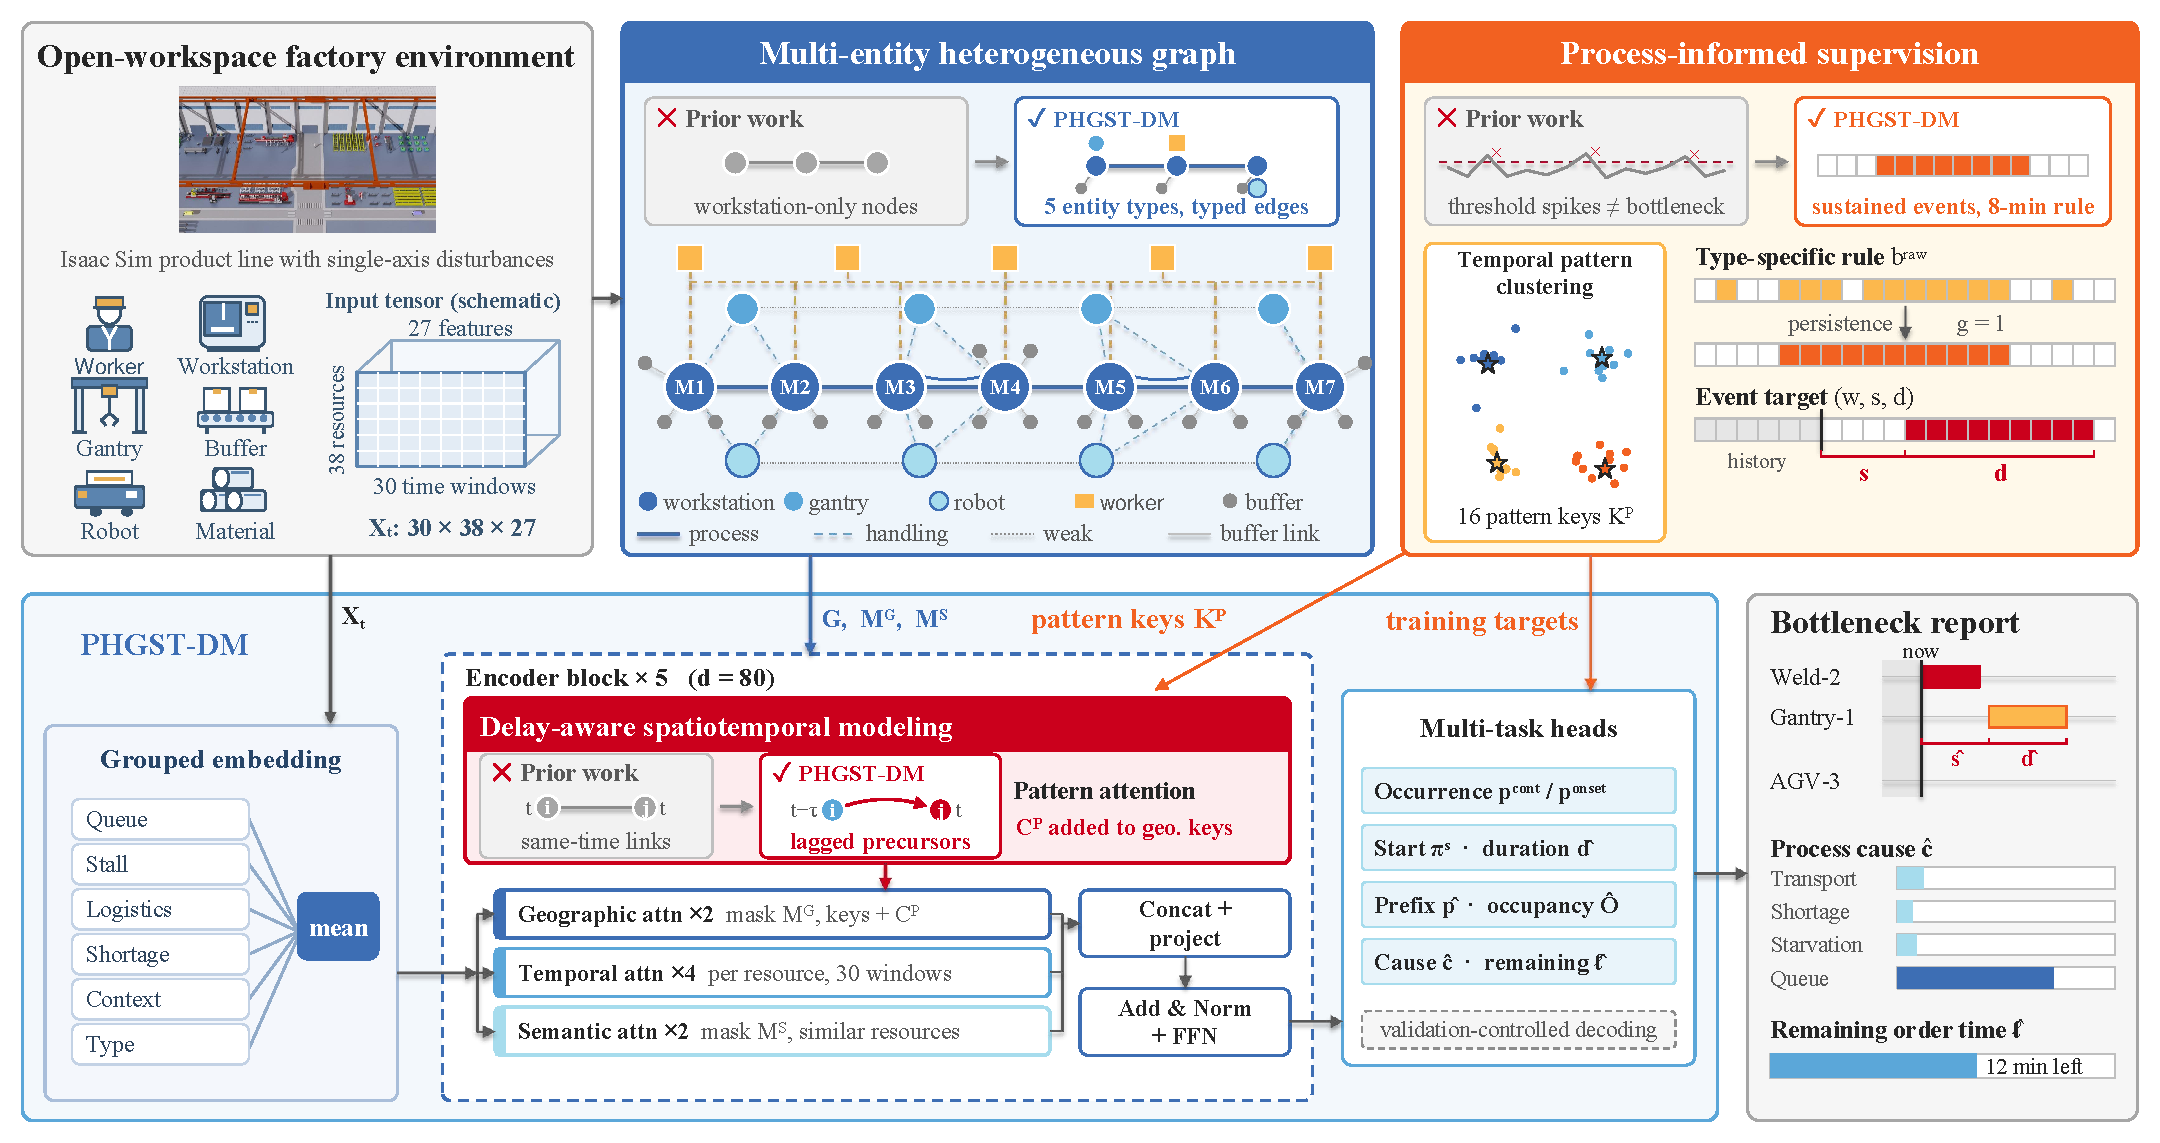
\includegraphics[width=\linewidth,height=0.58\textheight,keepaspectratio]{figures/fig_method_final.pdf}
\caption{Overall PHGST-DM framework: multi-entity observations, process-informed supervision, graph-based delay-aware encoding, and a structured bottleneck report.}
\label{fig:overview}
\end{figure}
\FloatBarrier

The model operates on production histories generated by a controlled factory process. Its role is to predict future constraints rather than to replace the admission, allocation, or task-planning controllers running the factory. Evaluation of the resulting forecasts is reported separately in Chapter~\ref{ch:experiments}.

Algorithm~\ref{alg:phgst-train} formalizes the complete training and model-selection pipeline. Algorithms~\ref{alg:targets}--\ref{alg:phgst-predict} detail its supervision, fixed context, and prediction steps. The retained event model and report threshold are specific to each onset-limit setting; the curriculum transfers a checkpoint between settings, while remaining-time specialization preserves each selected event operating point.

\begin{algorithm}[p]
\singlespacing
\footnotesize
\SetAlFnt{\footnotesize}
\SetAlCapFnt{\small}
\SetAlCapNameFnt{\small\bfseries}
\SetInd{0.5em}{0.8em}
\caption{End-to-end PHGST-DM training, selection, and held-out evaluation.}
\label{alg:phgst-train}
\KwIn{raw episodes $\mathcal{E}$; factory relations $G$; onset limits $\mathcal{H}=\{5,10,15\}$; candidate thresholds $\mathcal{T}$}
\KwOut{frozen event model $\theta^{\star}$, remaining-time head $\psi^{\star}$, threshold $\tau^{\star}$, held-out reports}
\BlankLine
\textbf{Phase 1: leakage-controlled data and fixed structural context}\;
split $\mathcal{E}$ by episode into $\mathcal{E}_{\mathrm{tr}},\mathcal{E}_{\mathrm{val}},\mathcal{E}_{\mathrm{te}}$\;
construct samples with history-only inputs using Algorithm~\ref{alg:targets}, independently within each episode\;
fit all feature/target scalers on $\mathcal{E}_{\mathrm{tr}}$; reuse them unchanged for $\mathcal{E}_{\mathrm{val}}$ and $\mathcal{E}_{\mathrm{te}}$\;
obtain $(A,M^{G},M^{S},E_{\mathrm{lap}})$ from Algorithm~\ref{alg:graph-masks} and $K^{P}$ from Algorithm~\ref{alg:pattern-bank}\;
freeze every data-derived structural quantity before neural-parameter optimization \tcp*{masks and prototypes stay fixed}
\BlankLine
\textbf{Phase 2: shared-representation learning (training stage 1)}\;
initialize $\theta$ from the documented prefix-supervised checkpoint\;
\ForEach{$H_{\mathrm{start}}\in\mathcal{H}$ in curriculum order}{
warm-start the current onset limit from the preceding retained checkpoint when available\;
  \For{epoch $=1,\ldots,E_1$ ($E_1=50$) until patience is exhausted}{
    \ForEach{oversampled training minibatch $B$}{
$(\widehat{Y}^{\mathrm{evt}},\hat O,\hat c,\hat\ell)\leftarrow\mathrm{PHGSTDMForward}_{\theta}(B,A,M^{G},M^{S},K^{P})$\;
evaluate the event, occupancy, cause, reconstruction, contrastive, and remaining-time losses, then update $\theta$\;
    }
decode $\mathcal{E}_{\mathrm{val}}$ with Algorithm~\ref{alg:phgst-predict} for every $\tau\in\mathcal{T}$\;
retain checkpoints and thresholds by the validation rules in Section~\ref{sec:experimental-settings}, including the validation-only fallback\;
  }
}
freeze the selected stage-1 parameters and threshold as $(\theta^{\star},\tau^{\star})$ \tcp*{event reports locked hereafter}
\BlankLine
\textbf{Phase 3: remaining-time specialization (training stage 2)}\;
freeze the encoder and all event, occupancy, and cause heads\;
initialize the rate-augmented remaining-time head $\psi$ from $\theta^{\star}$\;
\For{epoch $=1,\ldots,E_2$ ($E_2=20$) until validation loss stops improving}{
update only $\psi$ using progress-weighted remaining-time loss\;
}
freeze $\psi^{\star}$; do not retune $\tau^{\star}$\;
\BlankLine
\textbf{Phase 4: held-out evaluation after all choices are frozen}\;
run Algorithm~\ref{alg:phgst-predict} on $\mathcal{E}_{\mathrm{te}}$ using $(\theta^{\star},\psi^{\star},\tau^{\star})$\;
\Return frozen models, threshold, and held-out reports \tcp*{test episodes never re-enter selection}
\end{algorithm}
\FloatBarrier

\subsection{Production System and Resource Relations}\label{production-system-and-resource-relations}

The evaluated production system processes an order of ten workpieces through cutting, grooving, spot welding, root welding, surface welding, and finishing. The operation also involves worker service, intermediate storage, gantry handling, and AGV transportation. In this report, a \textbf{workstation} is a processing or assembly unit, including automated equipment and manually operated workbenches.

Let \(\mathcal{R}\) be the set of all resources, partitioned into workstations, gantries, transport robots, workers, and buffers:

\[
\mathcal{R}=\mathcal{R}^{m}\cup\mathcal{R}^{g}\cup\mathcal{R}^{a}\cup\mathcal{R}^{h}\cup\mathcal{R}^{b}.
\]

The evaluated graph contains 38 nodes. Event supervision is restricted to workstations, gantries, and AGVs:

\[
\mathcal{S}=\mathcal{R}^{m}\cup\mathcal{R}^{g}\cup\mathcal{R}^{a}.
\]

\begin{table}[!htbp]
\centering
\caption{Heterogeneous graph entities and their supervision roles.}
\label{tab:resources}
\small
\begin{tabularx}{\linewidth}{@{}l c X@{}}
\toprule
Resource type & Nodes & Role in the representation \\
\midrule
Workstations & 7 & Processing and assembly; event-supervised \\
Gantries & 4 & Handling services; event-supervised \\
Transport robots (AGVs) & 4 & Transportation; event-supervised \\
Workers & 5 & Labour availability and service context \\
Buffers & 18 & Storage and WIP context \\
\midrule
\textbf{Total} & \textbf{38} & \textbf{15 event-supervised resources} \\
\bottomrule
\end{tabularx}
\end{table}
\FloatBarrier

Worker and buffer nodes provide predictive context but are not assigned separate event targets. Materials are not added as independent graph nodes: their effects enter through shortage, inbound-waiting, and buffer-related features associated with existing resources.

The factory relations are represented by a \textbf{weighted undirected graph}:

\[
G=(\mathcal{R},E,A),\qquad E=E^{p}\cup E^{f}\cup E^{b}\cup E^{l}\cup E^{w},
\]

where \(A\) is the symmetric weighted adjacency matrix. The five edge groups represent process-chain links, parallel workstations in the same equipment family, buffer--workstation associations, handling--processing links, and same-type handling links, respectively. Edges encode structural relations that permit information exchange; they should not be interpreted as experimentally established physical causal pathways.

\subsection{Windowed State and Joint Prediction Targets}\label{windowed-state-and-joint-prediction-targets}

Operational records are aggregated into non-overlapping windows of \(\Delta=60\,\mathrm{s}\). Each resource has a 27-dimensional state vector \(x_{t,n}\in\mathbb{R}^{27}\), consisting of 21 operational variables, five resource-type indicators, and one labour-saturation variable. The operational features are divided into six semantic groups:

\begin{table}[!htbp]
\centering
\caption{Semantic feature groups in the final model.}
\label{tab:features}
\small
\begin{tabularx}{\linewidth}{@{}l c X@{}}
\toprule
Group & Dimension & Representative information \\
\midrule
Queue & 4 & Queue length, waiting, occupancy, growth \\
Stall & 6 & Blocked/starved time, stop, availability, coupling \\
Logistics & 4 & Departure variation, route/inbound delay, buffer \\
Shortage & 1 & Material-shortage propagation \\
Context & 7 & Activity, duration, time gap, operating variation, turning state, labour \\
Type & 5 & Workstation, gantry, worker, robot, buffer \\
\midrule
\textbf{Total} & \textbf{27} & \\
\bottomrule
\end{tabularx}
\end{table}
\FloatBarrier

Labour saturation is derived from worker states and provided to workstations. The exported \emph{offline bottleneck score} is \textbf{excluded} from predictive inputs, preventing the model from simply reproducing its own supervision score. With forecast origin \(t\), historical length \(T_{\mathrm{in}}=30\), and \(N=38\) nodes, the input is

\[
X_t=\bigl[x_{\tau,n}\bigr]_{\substack{\tau=t-T_{\mathrm{in}},\ldots,t-1\\n=1,\ldots,N}}
\in\mathbb{R}^{T_{\mathrm{in}}\times N\times27}
=\mathbb{R}^{30\times38\times27}.
\]

The future occupancy-label grid contains \(H_{\mathrm{label}}=30\) one-minute windows. A newly starting event is eligible for a report only if its onset lies within a separate \textbf{onset limit} \(H_{\mathrm{start}}\in\{5,10,15\}\) minutes. The onset limit restricts the admissible \emph{start} of a new event; it does not shorten the fixed 30-minute future label grid.

For supervised resource \(n\), the event target is

\[
y^{\mathrm{evt}}_{t,n}=(w_{t,n},s_{t,n},d_{t,n}),
\]

where \(w_{t,n}\) is event occurrence, \(s_{t,n}\) is onset offset, and \(d_{t,n}\) is future event length, all temporal quantities being expressed in one-minute windows. The model also estimates a graph-level process-cause class \(c\) and line-level remaining-order time \(\ell\).

The corresponding predictive mapping is

\[
f_{\theta}:(X_t,G)\longmapsto
\left(\{\hat w_{t,n},\hat s_{t,n},\hat d_{t,n}\}_{n\in\mathcal{S}},\;\hat c_t,\;\hat\ell_t\right),
\]

with parameters \(\theta\). Although the report is generated at \(t\), individual target construction and inference use different temporal information; Section~\ref{data-preparation-and-process-informed-supervision} makes that distinction explicit.

\section{Data Preparation and Process-informed Supervision}\label{data-preparation-and-process-informed-supervision}

\subsection{Open-workspace Factory Model and Data Collection}\label{open-workspace-factory-model-and-data-collection}

The NVIDIA Isaac Sim factory model records resource transitions, processing and job traces, buffer changes, transport tasks, and inventory at logical-second resolution. Streams are synchronized by episode identifier and logical time. In the evaluated setup, a completed episode contains ten finished workpieces. Episodes affected by the documented simulator deadlock defect are discarded as invalid records, rather than being used as normal production trajectories.

The data-generation environment supports configurable changes to \textbf{workstation}, \textbf{worker}, \textbf{logistics}, and \textbf{material} operating conditions. Each variation dimension can affect episode-wide capacity, sampled service behaviour, or temporary runtime events; the evaluated \texttt{dense\_i1} collection activates a single variation dimension at intensity level 1, alongside nominal episodes. Full disturbance settings, episode counts, and train/validation/test composition belong to Chapter~\ref{ch:experiments}. Critically, the category used to generate an operating variation is \emph{not} copied directly into the process-cause label: supervision is derived from observed states following the variation.

\begin{figure}[!htbp]
\centering
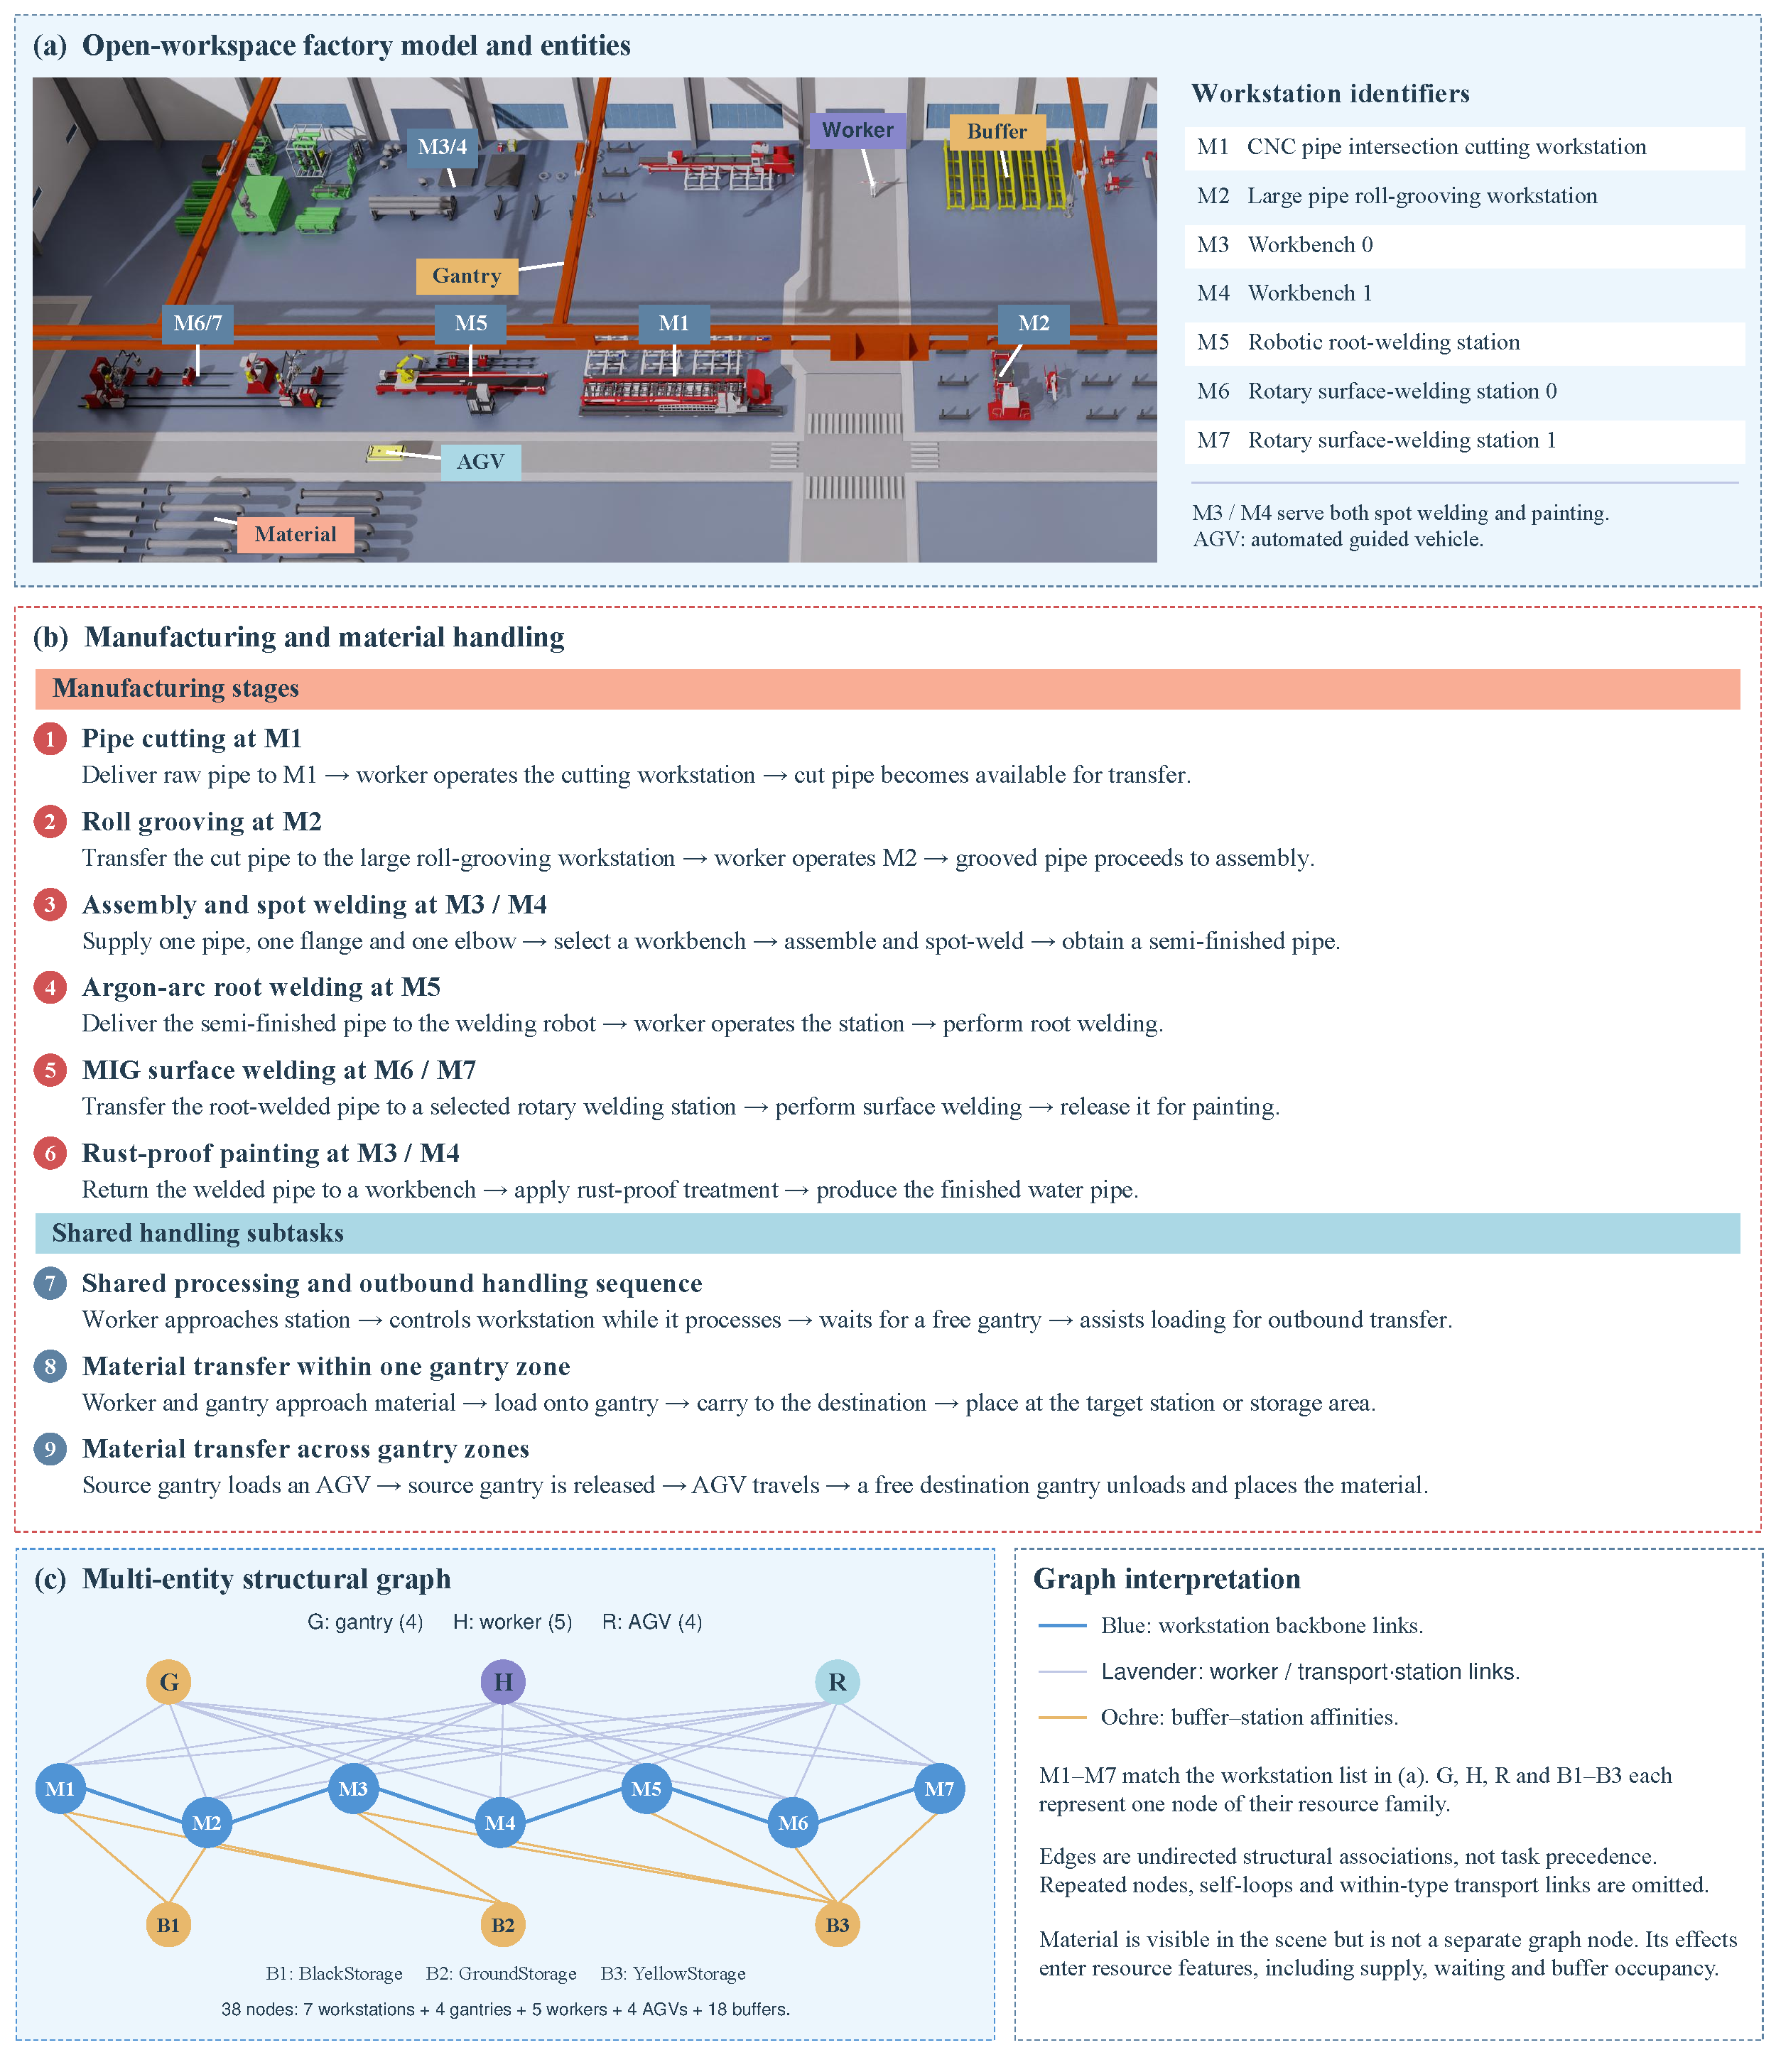
\includegraphics[width=\linewidth,height=0.70\textheight,keepaspectratio]{figures/fig_experiment.pdf}
\caption{Isaac Sim production environment, manufacturing and handling stages, and the heterogeneous graph of 38 resources.}
\label{fig:factory}
\end{figure}
\FloatBarrier

\subsection{Multi-entity Aggregation and Regime Context}\label{multi-entity-aggregation-and-regime-context}

Second-resolution logs are transformed into resource-by-window observations. Processing, blockage, starvation, and stoppage durations are accumulated according to their overlap with a 60-second window; activity and unavailability ratios are normalized by the window length. Queue statistics count waiting jobs and summarize waiting time. Buffer occupancy is averaged within the window, its previous value is carried forward when no update is recorded, and growth is computed from window-end minus window-start counts. Production and transport relations are used to derive coupling information, route delay, inbound waiting, and shortage propagation.

A fixed resource ordering aligns the heterogeneous channels across all episodes. Missing numeric entries are filled with zero, type indicators are appended, and labour saturation is recomputed from worker activity. Histories are generated using a one-window stride without crossing episode boundaries. Standardization is fitted \textbf{only on training histories} and reused unchanged for validation and testing.

The run-stratified episode split contains 140 training, 28 validation, and 36 test episodes, giving 20,826, 4,331, and 5,354 forecast windows, respectively (Table~\ref{tab:exp-dataset}). Splitting by complete episode precedes fitting scalers, semantic masks, and temporal prototypes; overlapping histories never cross episode boundaries. The disturbance protocol is specified in Table~\ref{tab:disturbance-design}, while baseline definitions and evaluation metrics are given in Tables~\ref{tab:exp-baselines} and~\ref{tab:exp-metrics}. These settings define the evaluation procedure without duplicating the results in Chapter~\ref{ch:experiments}.

The method distinguishes three related but non-equivalent objects. \textbf{Process-cause labels} represent observed operating symptoms accompanying bottleneck evidence. \textbf{Deterministic regime identifiers} are generated by cause-aligned rules to provide representation and contrastive-learning context. \textbf{Temporal-pattern prototypes} are clustered from training activity histories and subsequently used for attention conditioning (Section~\ref{recurrent-pattern-guided-delay-aware-spatiotemporal-modelling}). Neither regime IDs nor temporal clusters should be mistaken for independently verified bottleneck truth.

\subsection{Construction of Sustained Bottleneck Events}\label{construction-of-sustained-bottleneck-events}

Raw resource evidence must distinguish an operationally meaningful constraint from ordinary resource activity or a brief fluctuation. For resource type \(\rho(n)\), the rule \(\Phi_{\rho(n)}\) maps resource state and observed process information to a binary hot indicator:

\[
b^{\mathrm{raw}}_{t,n}=\Phi_{\rho(n)}(x_{t,n},X_t)\in\{0,1\}.
\]

Workstation evidence combines queue conditions, blockage/starvation, availability, coupling to upstream or downstream resources, inbound waiting, route delay, shortage propagation, and labour conditions. Gantry and AGV rules place greater emphasis on handling-related waiting and unavailability. The threshold conditions are applied to \textbf{physical-scale} features before standardization, rather than arbitrary normalized values. Table~\ref{tab:raw-hot} gives representative rules rather than an exhaustive list of workstation conditions.

\begin{table}[!htbp]
\centering
\caption{Selected examples of resource-specific raw-hot evidence (non-exhaustive). Here $q$ is queue length, $B$ blocked seconds, $S$ starved seconds, $I$ inbound-wait seconds, $R$ route-delay seconds, and $U$ unavailable fraction.}
\label{tab:raw-hot}
\small
\begin{tabularx}{\linewidth}{@{}p{2.35cm} X@{}}
\toprule
Resource & Representative raw-hot conditions (logical OR) \\
\midrule
Workstation & $q\geq2$ and $B+S>0$; or $B\geq24$ s and $q\geq1$; other stall/coupling/shortage/labour conditions also apply \\
Gantry & $B+S\geq18$ s and ($I\geq20$ s or $R\geq20$ s); or $U\geq0.5$ \\
AGV & $B+S\geq18$ s and $I\geq20$ s; or $U\geq0.5$ \\
\bottomrule
\end{tabularx}
\end{table}
\FloatBarrier

To remove transient positives, a short-run filter \(\mathcal{D}_m\) first drops raw positive runs shorter than \(m=8\) one-minute windows. A subsequent internal-gap operator \(\mathcal{F}_g\) fills gaps of at most \(g=1\) window between retained regions. The offline sustained occupancy sequence is therefore

\[
o_{:,n}=\mathcal{F}_{1}\!\left(\mathcal{D}_{8}\!\left(b^{\mathrm{raw}}_{:,n}\right)\right).
\]

The ordering matters: \textbf{short-run removal precedes internal gap filling}. This occupancy grid is an \emph{offline target} obtained from the full episode and may retrospectively use later observations to decide whether an earlier period belongs to a sustained event. At forecast origin \(t\), the predictor must instead use the \textbf{history-only} state \(h_{t-1,n}\) computed exclusively from windows strictly before \(t\), including prefix-based persistence and gap checks. In general, \(h_{t-1,n}\) need not equal the retrospective \(o_{t-1,n}\).

An event is \textbf{ongoing} if the history-only state is active and the future run starts at offset zero; its target duration is the remaining future length. A newly appearing run with positive onset offset is \textbf{upcoming} if its onset lies within \(H_{\mathrm{start}}\) and it satisfies the minimum-duration rule. Where multiple eligible runs are available for one resource, the \textbf{longest} qualifying run is selected, rather than always the earliest. This defines \(w_{t,n}\), \(s_{t,n}\), and \(d_{t,n}\) without providing future occupancy labels as model inputs.

\subsection{Process-cause and Remaining-order-time Targets}\label{process-cause-and-remaining-order-time-targets}

The window-level process-cause categories are

\[
\mathcal{C}=\{\text{material shortage},\;\text{transport delay},\;\text{queue buildup},\;\text{downstream blockage}\}.
\]

When several conditions are observed, the deterministic priority is \textbf{material shortage \(\succ\) transport delay \(\succ\) queue buildup \(\succ\) downstream blockage}. The labels reflect process symptoms derived from measured states, rather than direct copies of injected variation dimensions or verified physical root causes. Cause-loss supervision is applied only to windows containing reportable bottleneck evidence with a supported cause class.

There is an important time-index distinction. For a generic observed window \(u\), \(c_u\) describes the corresponding cause evidence. When the sample at forecast origin \(t\) is assembled, the algorithm attaches \(c_{t-1}\) and rule-derived regime context \(r_{t-1}\) from the \textbf{last observed window}. The graph-level cause head is trained on these observable operating conditions. It is therefore not valid to claim that this head independently establishes the root cause of an unknown future bottleneck.

The remaining-order-time target \(\ell_t\) counts the future one-minute windows required to complete the outstanding jobs, subject to the configured prediction limit. It is an order-level target rather than a separate bottleneck duration for each resource.

Algorithm~\ref{alg:targets} collects the supervision procedure. Slice notation \(a:b\) in this algorithm is half-open: histories end at \(t-1\), and the future grid covers \(t,\ldots,t+H_{\mathrm{label}}-1\). Thus \(O_{t,:,n}\) denotes resource \(n\)'s future occupancy within sample \(t\). The parameters are \(T_{\mathrm{in}}=30\), \(H_{\mathrm{label}}=30\), \(m=8\), and \(g=1\); no eligible run yields \((w,s,d)=(0,0,0)\). Prefix supervision measures the uninterrupted hot run from the first future window. This offline target is distinct from the history-only state \(h_{t-1}\).

\begin{algorithm}[p]
\singlespacing
\footnotesize
\SetAlFnt{\footnotesize}
\SetAlCapFnt{\small}
\SetAlCapNameFnt{\small\bfseries}
\SetInd{0.5em}{0.8em}
\caption{Process-informed supervision and regime-context construction.}
\label{alg:targets}
\KwIn{episode trajectories $\mathcal{E}$; resource types $\rho$; supervised set $\mathcal{S}$; $T_{\mathrm{in}}$; $H_{\mathrm{label}}$; $H_{\mathrm{start}}$; $m$; $g{=}1$}
\KwOut{samples with history-only inputs $\mathcal{D}=\{(X_t,O_t,Y_t^{\mathrm{evt}},c_{t-1},\ell_t,r_{t-1})\}_t$}
$\mathcal{D}\leftarrow\varnothing$\;
\ForEach{completed, reset-free episode $e\in\mathcal{E}$}{
  \tcp{Phase 1: synchronize heterogeneous observations}
aggregate raw streams into non-overlapping 60-s windows\;
align resource states by identifier and append type/context channels\;
preserve the episode boundary and compute jobs remaining\;
  \tcp{Phase 2: construct the persistent occupancy grid}
  \ForEach{$n\in\mathcal{S}$ and window $u$}{
$b^{\mathrm{raw}}_{u,n}\leftarrow\Phi_{\rho(n)}(x_{u,n})$ using queue, stall, availability, shortage, and logistics evidence\;
  }
  \ForEach{$n\in\mathcal{S}$}{
$o_{:,n}\leftarrow\mathcal{F}_{g}(\mathcal{D}_{m}(b^{\mathrm{raw}}_{:,n}))$ \tcp*{drop short runs, then fill gaps}
  }
  \tcp{Phase 3: derive process cause and regime context}
  \ForEach{window $u$ and resource $n$}{
assign $r_{u,n}$ by the deterministic cause-aligned state rules\;
  }
  \ForEach{window $u$ containing reportable hot evidence}{
assign $c_u$ by the priority shortage $\succ$ delay $\succ$ queue $\succ$ blockage\;
set the cause-loss weight to $1$ only when $c_u\in\mathcal{C}$\;
  }
  \tcp{Phase 4: instantiate one forecasting sample with history-only inputs}
  \For{$t\leftarrow T_{\mathrm{in}}$ \KwTo episode completion}{
$X_t\leftarrow x_{t-T_{\mathrm{in}}:t,:,:}$ and $O_t\leftarrow o_{t:t+H_{\mathrm{label}},:}$\;
compute $h_{t-1}$ from the observed prefix $x_{0:t,:,:}$ only \tcp*{no retrospective occupancy supplied to inference}
    \ForEach{$n\in\mathcal{S}$}{
$(s,d)\leftarrow$ longest hot run of $O_{t,:,n}$ whose onset is within $H_{\mathrm{start}}$\;
      \eIf{$h_{t-1,n}=1$ and $s=0$}{
$(w_{t,n},s_{t,n},d_{t,n})\leftarrow(1,0,d)$ \tcp*{ongoing remainder}
      }{
        \eIf{$0<s\le H_{\mathrm{start}}$ and $d\ge m$}{
$(w_{t,n},s_{t,n},d_{t,n})\leftarrow(1,s,d)$ \tcp*{upcoming event}
        }{
$(w_{t,n},s_{t,n},d_{t,n})\leftarrow(0,0,0)$\;
        }
      }
    }
$\ell_t\leftarrow$ future one-minute windows until all jobs finish, clipped by the prediction limit\;
append $(X_t,O_t,Y_t^{\mathrm{evt}},c_{t-1},\ell_t,r_{t-1})$ to $\mathcal{D}$\;
  }
}
\Return $\mathcal{D}$\;
\end{algorithm}
\FloatBarrier

\section{Heterogeneous Factory Graph and Input Representation}\label{heterogeneous-factory-graph-and-input-representation}

\subsection{Graph Instantiation and Attention Masks}\label{graph-instantiation-and-attention-masks}

The five resource-relation families introduced in Section~\ref{overall-framework-and-problem-formulation} are assigned fixed adjacency weights of \(1.0\), \(0.8\), \(0.6\), \(0.5\), and \(0.3\), respectively, and self-loops have weight \(1.0\). Relation entries are symmetrized in \(A\). The graph retains the manufacturing interpretation of structural connections while the encoder constructs different masks for graph proximity and behaviour similarity.

The \textbf{geographic mask} uses the shortest-path hop distance \(D^{\mathrm{hop}}_{ij}\) computed by Floyd--Warshall. With cutoff \(\delta_G=4\),

\[
M^G_{ij}=\begin{cases}
0,&D^{\mathrm{hop}}_{ij}<\delta_G,\\
-\infty,&\text{otherwise},
\end{cases}\qquad\delta_G=4.
\]

Zero permits an attention connection, while \(-\infty\) blocks it in the softmax. Thus the geographic branch attends to nodes fewer than four hops away.

The \textbf{semantic mask} uses the similarity of training-only resource histories. If \(\bar{x}_{:,i}\) denotes the channel-averaged training trajectory of resource \(i\), the distance is

\[
D^{\mathrm{sem}}_{ij}=1-\operatorname{corr}(\bar{x}_{:,i},\bar{x}_{:,j}).
\]

For each resource, its five closest trajectories under this Pearson-correlation distance are retained as semantic neighbours together with the self-connection. Unlike traffic PDFormer's dynamic-time-warping similarity, this implementation uses Pearson correlation for its short-episode data. The masks are fixed from training information and are not recomputed on held-out test trajectories.

Graph structure is additionally encoded through the normalized Laplacian

\[
L=I-D_A^{-1/2}AD_A^{-1/2},
\]

where \(D_A\) is diagonal with entries equal to adjacency row sums. Eight nontrivial eigenvectors provide structural positional features. The adjacency, geographic mask, semantic mask, Laplacian positions, and temporal prototype bank are fixed before neural-parameter optimization.

Algorithm~\ref{alg:graph-masks} gives the graph construction explicitly. Here \(\mathcal{V}\) is the resource-node set (the \(\mathcal{R}\) of the problem formulation), whereas the algorithm's typed-relation list \(\mathcal{R}\) contains triples \((i,j,w)\). Repeated relations retain their maximum weight; semantic-neighbour selection considers finite correlation distances and retains the self-connection.

\begin{algorithm}[p]
\singlespacing
\footnotesize
\SetAlFnt{\footnotesize}
\SetAlCapFnt{\small}
\SetAlCapNameFnt{\small\bfseries}
\SetInd{0.5em}{0.8em}
\caption{Factory graph and attention-mask construction.}
\label{alg:graph-masks}
\KwIn{resources $\mathcal{V}$; typed relations $\mathcal{R}$; scaled training histories $X^{\mathrm{tr}}$; $\delta_G{=}4$; $k_S{=}5$; $d_{\mathrm{lap}}{=}8$}
\KwOut{weighted adjacency $A$; geographic mask $M^G$; semantic mask $M^S$; structural positions $E_{\mathrm{lap}}$}
$A\leftarrow I_{|\mathcal{V}|}$\;
\ForEach{typed relation $(i,j,w)\in\mathcal{R}$}{
$A_{ij}\leftarrow A_{ji}\leftarrow\max(A_{ij},w)$\;
}
$D^{\mathrm{hop}}\leftarrow\mathrm{FloydWarshall}(\mathbf{1}[A>0])$\;
\ForEach{$(i,j)\in\mathcal{V}\times\mathcal{V}$}{
$M^G_{ij}\leftarrow0$ if $D^{\mathrm{hop}}_{ij}<\delta_G$, otherwise $-\infty$\;
}
$\bar x_{:,i}\leftarrow\mathrm{MeanChannels}(X^{\mathrm{tr}}_{:,:,i,:})$ for every $i$\;
$D^{\mathrm{sem}}_{ij}\leftarrow1-\mathrm{corr}(\bar x_{:,i},\bar x_{:,j})$\;
\ForEach{$i\in\mathcal{V}$}{
$\mathcal{N}^{S}_i\leftarrow$ indices of the $k_S$ smallest finite values in $D^{\mathrm{sem}}_{i,:}$\;
$M^S_{ij}\leftarrow0$ for $j\in\mathcal{N}^{S}_i\cup\{i\}$, and $-\infty$ otherwise\;
}
$L\leftarrow I-D_A^{-1/2}AD_A^{-1/2}$\;
$E_{\mathrm{lap}}\leftarrow$ first $d_{\mathrm{lap}}$ nontrivial eigenvectors of $L$\;
\Return $A,M^G,M^S,E_{\mathrm{lap}}$\;
\end{algorithm}
\FloatBarrier

\subsection{Grouped Heterogeneous State Embedding}\label{grouped-heterogeneous-state-embedding}

The 27 input features have different operational meanings and are projected through \textbf{six separate semantic groups}, rather than a single undifferentiated linear layer. For group \(q\),

\[
e^{(q)}_{t,n}=\operatorname{GELU}\!\left(W_qx^{(q)}_{t,n}+b_q\right).
\]

The six projected embeddings are averaged,

\[
e_{t,n}=\frac{1}{6}\sum_{q=1}^{6}e^{(q)}_{t,n},
\]

so each semantic group contributes equally regardless of its original channel count. The initial spatiotemporal representation incorporates this grouped embedding, sinusoidal time positions, projected graph-Laplacian positions, and learned node identities:

\[
H^{(0)}=E_{\mathrm{group}}(X_t)+E_{\mathrm{time}}+E_{\mathrm{lap}}(G)+E_{\mathrm{node}}.
\]

Day-of-week and time-of-day embeddings are disabled because the evaluated episodes are governed by order progress and operating variations, not a calendar periodicity.

\section{Recurrent-pattern-guided Delay-aware Spatiotemporal Modelling}\label{recurrent-pattern-guided-delay-aware-spatiotemporal-modelling}

\begin{figure}[!htbp]
\centering
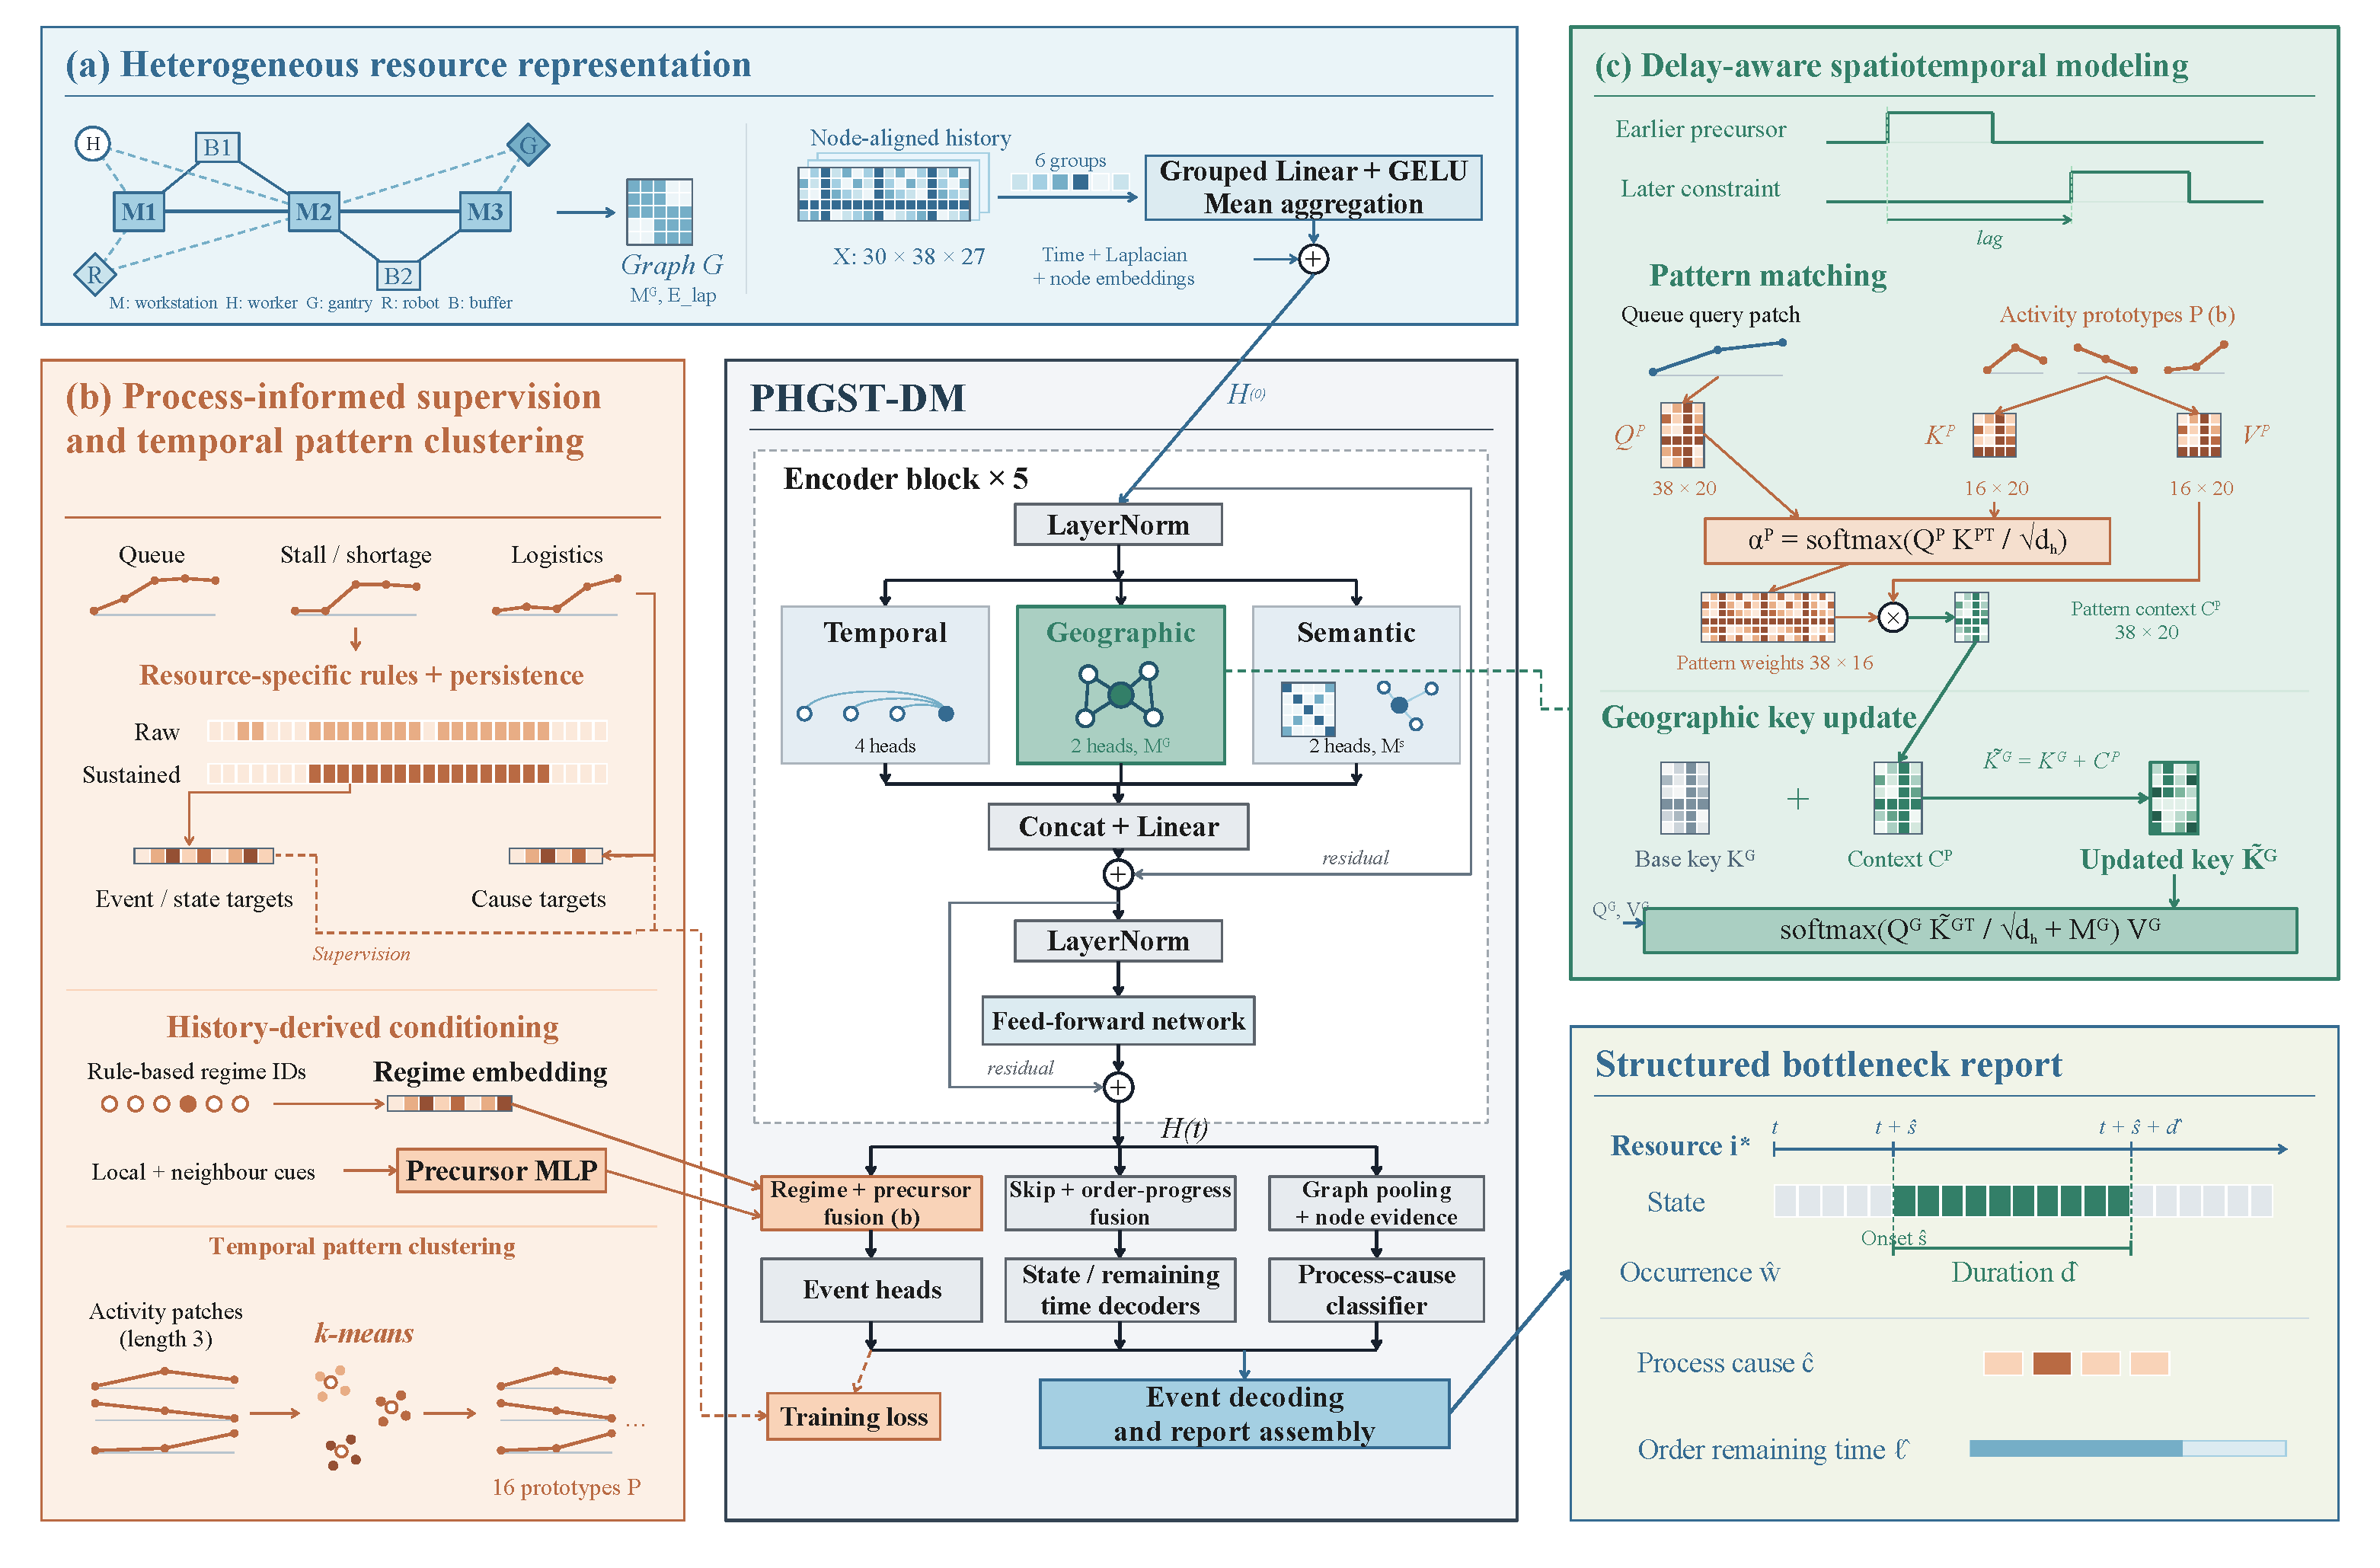
\includegraphics[width=\linewidth,height=0.62\textheight,keepaspectratio]{figures/fig_model_final.pdf}
\caption{PHGST-DM architecture and recurrent-pattern-guided geographic-attention conditioning.}
\label{fig:architecture}
\end{figure}
\FloatBarrier

\subsection{Temporal, Geographic, and Semantic Attention}\label{temporal-geographic-and-semantic-attention}

PHGST-DM uses temporal, geographic, and semantic branches in each encoder block, following the general spatiotemporal-attention design of PDFormer~\cite{jiang2023pdformer} but applying it to heterogeneous manufacturing states and relations. For branch \(b\in\{T,G,S\}\), the scaled dot-product operation is

\[
\operatorname{Attn}_b(Q_b,K_b,V_b;M_b)=
\operatorname{softmax}\!\left(\frac{Q_bK_b^{\top}}{\sqrt{d_h}}+M_b\right)V_b,
\]

where \(d_h\) is the per-head query/key dimension. The temporal branch learns dependencies within each resource's historical windows. Geographic attention uses \(M^G\) and the factory's structural neighbourhood; semantic attention uses \(M^S\) and training-history similarity. Their outputs are concatenated and projected, then processed by pre-normalized residual and feed-forward layers.

Five encoder blocks are used, each with hidden dimension \(80\). The temporal, geographic, and semantic branches contain \textbf{4, 2, and 2 heads}, respectively. A further operating-pattern context \(C^P\) conditions the geographic branch; it is defined next.

\subsection{Training-only Temporal Pattern Clustering}\label{training-only-temporal-pattern-clustering}

To summarize recurrent temporal behaviour, the model constructs a fixed prototype bank using K-means on \textbf{three-window activity-ratio patches from training histories}. The bank contains \(K=16\) prototypes, each of length \(S=3\) windows. Training-fitted feature scaling is used, the clustering initialization seed is \(0\), and the specified procedure performs ten iterations. For a patch \(p\), assignment to prototype \(k\) minimizes squared Euclidean distance:

\[
a(p)=\arg\min_{k}\lVert p-k_k^P\rVert_2^2,
\qquad
k_k^P=\frac{1}{|\mathcal{P}_k|}\sum_{p\in\mathcal{P}_k}p.
\]

The resulting pattern bank \(K^P=\{k_1^P,\dots,k_{16}^P\}\) is kept fixed during downstream model training and evaluation. These are \textbf{recurrent operating-pattern prototypes}, not labels for bottleneck presence or process causes.

Algorithm~\ref{alg:pattern-bank} specifies initialization, assignment, and centre updates. Its patch slice \(u:u+S-1\) includes both endpoints and therefore contains exactly \(S=3\) windows. Centres with no assigned patches remain unchanged, as only nonempty assignment sets are updated.

\begin{algorithm}[p]
\singlespacing
\footnotesize
\SetAlFnt{\footnotesize}
\SetAlCapFnt{\small}
\SetAlCapNameFnt{\small\bfseries}
\SetInd{0.5em}{0.8em}
\caption{Training-only temporal pattern clustering.}
\label{alg:pattern-bank}
\KwIn{scaled training histories $X^{\mathrm{tr}}$; activity channel $c_{\mathrm{act}}$; patch length $S{=}3$; centres $K{=}16$; iterations $J{=}10$; seed $0$}
\KwOut{pattern bank $K^P=\{k^P_1,\ldots,k^P_K\}$}
$\mathcal{P}\leftarrow\varnothing$\;
\ForEach{training history $X_b\in X^{\mathrm{tr}}$}{
  \ForEach{resource $n$ and valid start $u$}{
append $X_{b,u:u+S-1,n,c_{\mathrm{act}}}$ to $\mathcal{P}$\;
  }
}
initialize $K^P$ with $K$ distinct patches sampled from $\mathcal{P}$ using seed $0$\;
\For{$j=1,\ldots,J$}{
assign each $p\in\mathcal{P}$ to $a(p)=\arg\min_k\lVert p-k^P_k\rVert_2^2$\;
  \ForEach{centre $k$ with a nonempty assignment set $\mathcal{P}_k$}{
$k^P_k\leftarrow |\mathcal{P}_k|^{-1}\sum_{p\in\mathcal{P}_k}p$\;
  }
}
\Return $K^P$ reshaped to $K\times S\times1$\;
\end{algorithm}
\FloatBarrier

\subsection{Pattern-conditioned Cross-resource Interaction}\label{pattern-conditioned-cross-resource-interaction}

At prediction time, the query \(P_{t,n}\) is a \textbf{three-window queue-length patch} from the observed history, whereas the keys and values originate from the fixed \textbf{activity-ratio} prototype bank. The pattern context is

\[
C^P_{t,n}=\operatorname{softmax}\!\left(
\frac{f_Q^P(P_{t,n})\,f_K^P(K^P)^{\top}}{\sqrt{d_h}}
\right)f_V^P(K^P).
\]

The projections \(f_Q^P\), \(f_K^P\), and \(f_V^P\) are learned, but the prototype centres themselves stay fixed. The context \(C^P\) is added to the \textbf{geographic attention keys}, conditioning graph-based resource interaction on recent queue evolution matched to recurrent activity patterns. At block \(l\) the three streams may therefore be written as

\[
\begin{aligned}
H_T^{(l)}&=\operatorname{Attn}_T(H^{(l-1)}),\\
H_G^{(l)}&=\operatorname{Attn}_G(H^{(l-1)},M^G,C^P),\\
H_S^{(l)}&=\operatorname{Attn}_S(H^{(l-1)},M^S).
\end{aligned}
\]

The mechanism matches historical patches directly, \textbf{without Fourier transformation} and \textbf{without a supervised physical propagation-delay target}. It can exploit lagged predictive associations across resources, but attention maps alone are not causal explanations of how disturbances physically travel through the factory.

\section{Multi-task Bottleneck Prediction and Optimization}\label{multi-task-bottleneck-prediction-and-optimization}

\subsection{Event, Occupancy, and Explanatory Heads}\label{event-occupancy-and-explanatory-heads}

The final encoder representation is combined with deterministic regime context and local/neighbourhood precursor evidence to obtain a supervised-resource event representation \(z_{t,n}\). The model separates the prediction of an existing event's \textbf{continuation} from the \textbf{onset} of a new event:

\[
p^{\mathrm{cont}}_{t,n}=\sigma\!\left(f_{\mathrm{cont}}(z_{t,n})\right),\qquad
p^{\mathrm{onset}}_{t,n}=\sigma\!\left(f_{\mathrm{onset}}(z_{t,n})\right).
\]

The history-only state \(h_{t-1,n}\) selects the appropriate occurrence head during decoding. Additional heads produce an onset-offset distribution, predicted future duration, and prefix length:

\[
\begin{aligned}
\pi^s_{t,n}&=\operatorname{softmax}(f_s(z_{t,n})),\\
\hat d_{t,n}&=\operatorname{softplus}(f_d(z_{t,n})),\\
\hat p_{t,n}&=\operatorname{softplus}(f_p(z_{t,n})).
\end{aligned}
\]

The prefix length describes uninterrupted occupancy from the first future window and helps distinguish continued constraint from near-immediate recovery. A dense decoder predicts \(\hat O_t\in[0,1]^{H_{\mathrm{label}}\times N}\), providing future-window occupancy supervision in addition to event-level estimates.

Process-cause and remaining-order-time outputs are defined at graph level. Final node representations are pooled through a mean operation and a maximum gated-node score, then combined with order-progress information:

\[
u_t=\operatorname{AuxPool}(H_t^{(L)},\text{order state}),\qquad
\hat c_t=f_c(u_t),\quad\hat\ell_t=f_\ell(u_t).
\]

The cause head estimates rule-defined observed process conditions (Section~\ref{process-cause-and-remaining-order-time-targets}); it is not a ground-truth physical root-cause diagnosis. The remaining-time head estimates order-level progress rather than a second station-event duration.

\subsection{Joint Training Objective}\label{joint-training-objective}

The training objective combines event occurrence, onset, temporal regression, occupancy, auxiliary outputs, and representation regularization:

\[
\begin{aligned}
\mathcal{L}={}&\lambda_w\mathcal{L}_{\mathrm{will}}+\lambda_{on}\mathcal{L}_{\mathrm{onset}}+
\lambda_s\mathcal{L}_{\mathrm{start}}+\lambda_d\mathcal{L}_{\mathrm{dur}}\\
&+\lambda_p\mathcal{L}_{\mathrm{prefix}}+\lambda_o\mathcal{L}_{\mathrm{occ}}+
\lambda_{\ell}\mathcal{L}_{\mathrm{remain}}+\lambda_c\mathcal{L}_{\mathrm{cause}}\\
&+\lambda_r\mathcal{L}_{\mathrm{recon}}+\lambda_q\mathcal{L}_{\mathrm{contrast}}+
\lambda_{\mathrm{tpm}}\mathcal{L}_{\mathrm{tpm}}.
\end{aligned}
\]

Occurrence prediction combines reweighted binary cross-entropy, focal modulation, hard-false-positive weighting, and an internal differentiable F1 term. The new-onset head receives separate onset supervision. A Gaussian soft target supports onset-offset prediction, while log-transformed Smooth-L1 losses are used for duration, prefix, and remaining-time regression. The occupancy objective combines type-balanced binary cross-entropy with soft Dice and soft intersection-over-union terms. Class-weighted process-cause cross-entropy is applied only where a supported cause label accompanies positive bottleneck evidence. Reconstruction and supervised contrastive losses regularize the shared representation, and an auxiliary turning-point loss is included in the final objective.

One naming distinction matters for reproducing the configuration. The active event-occurrence term \(\mathcal{L}_{\mathrm{will}}\) is \textbf{not} the same as the disabled legacy configuration switch named \texttt{will}. The offline cluster-head weight is zero, \(\lambda_{\mathrm{cluster}}=0\), so the model is not trained to classify offline cluster assignments. Key loss weights and decoding thresholds are specified in Section~\ref{sec:experimental-settings}.

\subsection{Two-stage Training and Validation-controlled Decoding}\label{two-stage-training-and-validation-controlled-decoding}

\textbf{Stage 1: joint representation and event learning.} Training initializes the model from the documented prefix-supervised checkpoint and follows the onset-limit curriculum \(5\rightarrow10\rightarrow15\) minutes. When available, the retained checkpoint from one onset-limit setting warm-starts the next. Fourfold positive-window oversampling addresses the rarity of event-bearing samples. Far-onset enhancement and weighted false-positive penalties balance warning sensitivity against false reports. The optimizer is AdamW with batch size 16, an initial learning rate of \(5\times10^{-5}\), weight decay \(0.05\), and cosine decay towards \(10^{-6}\). The shared training protocol uses at most 50 epochs per onset-limit run and early-stopping patience 40.

\textbf{Validation selection.} Candidate checkpoints and report thresholds are evaluated only on the validation episodes. Checkpoint selection uses specified precision/recall gates and station-identification F1, with a validation-only fallback when the gates cannot be met. Candidate report thresholds are drawn from the documented set from 0.45 through 0.94. Once selected, the event model and threshold are frozen before any held-out test evaluation.

\textbf{Stage 2: remaining-time specialization.} The encoder and event, occupancy, and cause heads are frozen, while a rate-augmented remaining-time head is optimized using a progress-weighted objective. This stage does not retune the event threshold and does not change the frozen event or cause outputs. The finalized study uses seed 42; its principal experiments are single-seed estimates rather than multi-seed uncertainty measurements.

\textbf{Inference and report generation.} The decoder uses the observed-prefix state \(h_{t-1,n}\) to select the continuation score for an active resource or the new-onset score otherwise. Prefix evidence may retain an ongoing event with onset offset zero. An eligible occupancy run is extracted from the predicted occupancy grid and combined with event-head estimates under the appropriate duration rules. Global and resource-type thresholds, together with the active onset limit, determine which reports are retained. Each retained report contains resource identity, onset, predicted duration, the graph-level process-cause output, and remaining order time.

For strict evaluation, a matched report must identify the correct resource and satisfy an onset-offset tolerance of three one-minute windows:

\[
|\hat s_{t,n}-s_{t,n}|\leq\epsilon_s,\qquad \epsilon_s=3\ \mathrm{min}.
\]

This onset-qualified event metric is distinct from the internal station-identification score used during validation selection. Chapter~\ref{ch:experiments} details the evaluation results. Throughout the pipeline, held-out episodes are not used to fit scalers, masks, prototypes, neural parameters, or reporting thresholds.

Algorithm~\ref{alg:phgst-predict} formalizes the forward pass and report decoder. The symbols \(a_n^{\mathrm{cont}}\) and \(a_n^{\mathrm{onset}}\) denote head scores; their sigmoid probabilities correspond to \(p^{\mathrm{cont}}\) and \(p^{\mathrm{onset}}\). The residual updates abbreviate the pre-normalized encoder described in Section~\ref{temporal-geographic-and-semantic-attention}. The observed-prefix continuation cutoff is 1.5 windows, and occupancy runs use cutoff 0.45. Upcoming reports obey the onset limit and minimum-duration rule; ongoing duration describes the future remainder. Section~\ref{sec:experimental-settings} supplies the global and resource-type thresholds and full loss settings.

\begin{algorithm}[p]
\singlespacing
\footnotesize
\SetAlFnt{\footnotesize}
\SetAlCapFnt{\small}
\SetAlCapNameFnt{\small\bfseries}
\SetInd{0.5em}{0.8em}
\caption{PHGST-DM prediction with delay-aware spatiotemporal modelling.}
\label{alg:phgst-predict}
\KwIn{history $X_t$ and history-only state $h_{t-1}$; $A,M^{G},M^{S}$; pattern bank $K^{P}$; regime state $r_{t-1}$; parameters $(\theta,\psi)$; threshold $\tau$; onset limit $H_{\mathrm{start}}$}
\KwOut{station reports $\widehat{\mathcal{R}}_t$; occupancy $\hat O_t$; cause $\hat c_t$; remaining time $\hat\ell_t$}
\BlankLine
\textbf{Phase 1: heterogeneous state representation}\;
\ForEach{group $q$}{
$e^{(q)}\leftarrow\mathrm{GELU}(W_q x^{(q)}+b_q)$\;
}
$H^{(0)}\leftarrow\mathrm{mean}_{q}e^{(q)}+E_{\mathrm{time}}+E_{\mathrm{lap}}+E_{\mathrm{node}}$\;
construct history-only queue patches $P$ of length $3$ and project the fixed activity-pattern centres $K^{P}$\;
\BlankLine
\textbf{Phase 2: delay-aware spatiotemporal modelling}\;
\For{$l\leftarrow 1$ \KwTo $5$}{
$H_T\leftarrow\mathrm{Attn}_{T}(H^{(l-1)})$\;
$C^{P}\leftarrow\mathrm{softmax}(f_Q^{P}(P)f_K^{P}(K^{P})^{\top}/\sqrt{d_h})f_V^{P}(K^{P})$ \tcp*{queue query vs.\ activity prototypes}
$H_G\leftarrow\mathrm{Attn}_{G}(H^{(l-1)},M^{G};\,\text{geographic keys}+C^{P})$ \tcp*{delay-aware geographic mixing}
$H_S\leftarrow\mathrm{Attn}_{S}(H^{(l-1)},M^{S})$\;
$\widetilde H^{(l)}\leftarrow H^{(l-1)}+\mathrm{Proj}[H_T;H_G;H_S]$\;
$H^{(l)}\leftarrow\widetilde H^{(l)}+\mathrm{FFN}(\widetilde H^{(l)})$\;
}
\BlankLine
\textbf{Phase 3: station-level and graph-level prediction heads}\;
$z_n\leftarrow H^{(5)}_{t-1,n}+E_{\mathrm{regime}}(r_{t-1,n})$ for the station-event branch\;
fuse local queue/stall and neighbourhood precursor evidence into $z_n$\;
\ForEach{$n\in\mathcal{S}$}{
$(a^{\mathrm{cont}}_n,a^{\mathrm{onset}}_n)\leftarrow(f_{\mathrm{cont}}(z_n),f_{\mathrm{onset}}(z_n))$ \tcp*{continuation vs.\ new-onset scores}
$(\pi^{s}_n,\hat d_n,\hat p_n)\leftarrow(\mathrm{softmax}(f_s(z_n)),\mathrm{softplus}(f_d(z_n)),\mathrm{softplus}(f_p(z_n)))$\;
}
$\hat O_t\leftarrow\sigma(f_O(H^{(5)}))$; pool nodes and order progress into $u_t$; set $(\hat c_t,\hat\ell_t)\leftarrow(f_c(u_t),f_{\psi}(u_t))$\;
\BlankLine
\textbf{Phase 4: event-consistent operational decoding}\;
$\widehat{\mathcal{R}}_t\leftarrow\varnothing$\;
\ForEach{$n\in\mathcal{S}$}{
select $a_n\leftarrow a^{\mathrm{cont}}_n$ if $h_{t-1,n}=1$, and $a_n\leftarrow a^{\mathrm{onset}}_n$ otherwise\;
  \If{$h_{t-1,n}=1$ and $\hat p_n$ satisfies the continuation rule}{
lift $a_n$ with prefix evidence and set $\hat s_n\leftarrow0$\;
  }
recover the longest eligible run $(\hat s^{O}_n,\hat d^{O}_n)$ from $\hat O_{t,:,n}$\;
merge the run and event-head estimates subject to the ongoing/upcoming duration rule\;
apply the global threshold $\tau$, the resource-type threshold, and the onset limit $H_{\mathrm{start}}$\;
  \If{station $n$ is retained}{
append $(n,\hat s_n,\hat d_n,\hat c_t,\hat\ell_t)$ to $\widehat{\mathcal{R}}_t$\;
  }
}
\Return $\widehat{\mathcal{R}}_t,\hat O_t,\hat c_t,\hat\ell_t$\;
\end{algorithm}
\FloatBarrier

\section{Production-sensitivity Validation Protocol}\label{production-sensitivity-validation-protocol}

Predictive agreement with process-informed labels alone does not establish that the labels rank resources according to their influence on production completion. To examine this question, the study separately performs a counterfactual \textbf{production-sensitivity replay}. This procedure is independent of PHGST-DM training and inference.

At saved factory state \(t\), each of seven workstation candidates is evaluated through a separate service-bundle acceleration. Workstation processing and associated worker service durations are multiplied by \(0.8\), corresponding to a \(1.25\times\) service rate, for 1,200 simulation steps. Baseline and intervention branches start from the same saved factory and random-number states and run until order completion. For workstation \(i\), sensitivity is the reduction in remaining completion time:

\[
S_i(t)=M_{\mathrm{base}}(t)-M_{i,0.8}(t),
\]

where \(M_{\mathrm{base}}(t)\) and \(M_{i,0.8}(t)\) are measured from the same origin. Positive \(S_i(t)\) means that the specified temporary acceleration shortens the order's completion time.

Label-based rankings are formed using the maximum evidence in the last three fully observed windows before \(t\). Their alignment with counterfactual sensitivity is evaluated using \textbf{NDCG@3}, \textbf{Positive Recall@\(k\)}, \textbf{Weighted Recall@3}, and \textbf{Coverage@3} under a 90\%-of-maximum sensitivity criterion. NDCG@3 evaluates ranked relevance; Positive Recall@\(k\) covers the oracle's highest positive-sensitivity candidates; Weighted Recall@3 captures the proportion of total positive sensitivity ranked among the first three; and Coverage@3 assesses whether near-maximally sensitive resources appear among the first three candidates.

The protocol tests whether the operational labels agree with a specific, fixed acceleration intervention in the simulated factory. It does \textbf{not} demonstrate a general causal explanation of bottleneck events, the effectiveness of a learned intervention policy, or throughput improvement from forecast-guided closed-loop control. Its pilot results are presented in Section~\ref{sec:supervision-analysis}, while generalization limits and future validation directions are discussed in Chapter~\ref{ch:conclusion}.

In summary, the methodology brings together multi-entity factory observations, process-informed persistent-event supervision, a weighted heterogeneous process--logistics graph, and recurrent-pattern-conditioned spatiotemporal attention. It predicts resource-level event occurrence and timing together with observable process context and order progress, while maintaining a strict boundary between retrospective supervision and information available at the forecast origin.


% ==================== 已迁移：第 4--6 章 ====================
% Adapted from PHGST-DM_article_source/main.tex, original Section 5.
\chapter{Experiments and Analysis}
\label{ch:experiments}
\label{sec:exp}

The Process-Informed Heterogeneous-Graph Spatiotemporal Transformer with Delay-aware Modeling (PHGST-DM) jointly predicts the bottleneck station, onset, duration, observable process cause, and remaining order time. Its inputs combine resource observations on a heterogeneous process--logistics graph with recurrent temporal-pattern context.

We evaluate whether PHGST-DM can address limitations in observation scope and bottleneck supervision when forecasting bottleneck events, process causes, and remaining order time. Baseline comparisons evaluate these joint outputs; component studies examine heterogeneous multi-entity representation, process-informed supervision and temporal pattern clustering, and recurrent-pattern-guided delay-aware modelling. A case study follows bottleneck onset, persistence, and recovery. Together, these evaluations assess how the proposed designs contribute to advance warning and joint forecasting. Supplementary results and attention analyses are reported in Appendices~\ref{app:supplementary-results} and~\ref{app:attention-analysis}.

\FloatBarrier
\section{Experimental setup}

\subsection{Dataset and data processing}

Experiments use \texttt{dense\_i1}, collected from an open-workspace factory model developed in NVIDIA Isaac Sim. This dataset identifier denotes the collection with one active operating-variation dimension at intensity level 1, together with nominal episodes. Each episode produces ten workpieces through cutting, grooving, spot welding, root welding, surface welding, and finishing (Figure~\ref{fig:experiment}). The graph contains 38 nodes: seven workstations, four gantries, five workers, four transport robots (AGVs), and 18 buffers. The seven workstations, four gantries, and four AGVs are the 15 prediction targets; worker, buffer, and resource-associated material features supply context. Each resource is represented by 27 features, and observations are aggregated into one-minute windows.

\begin{figure}[!htbp]
\centering
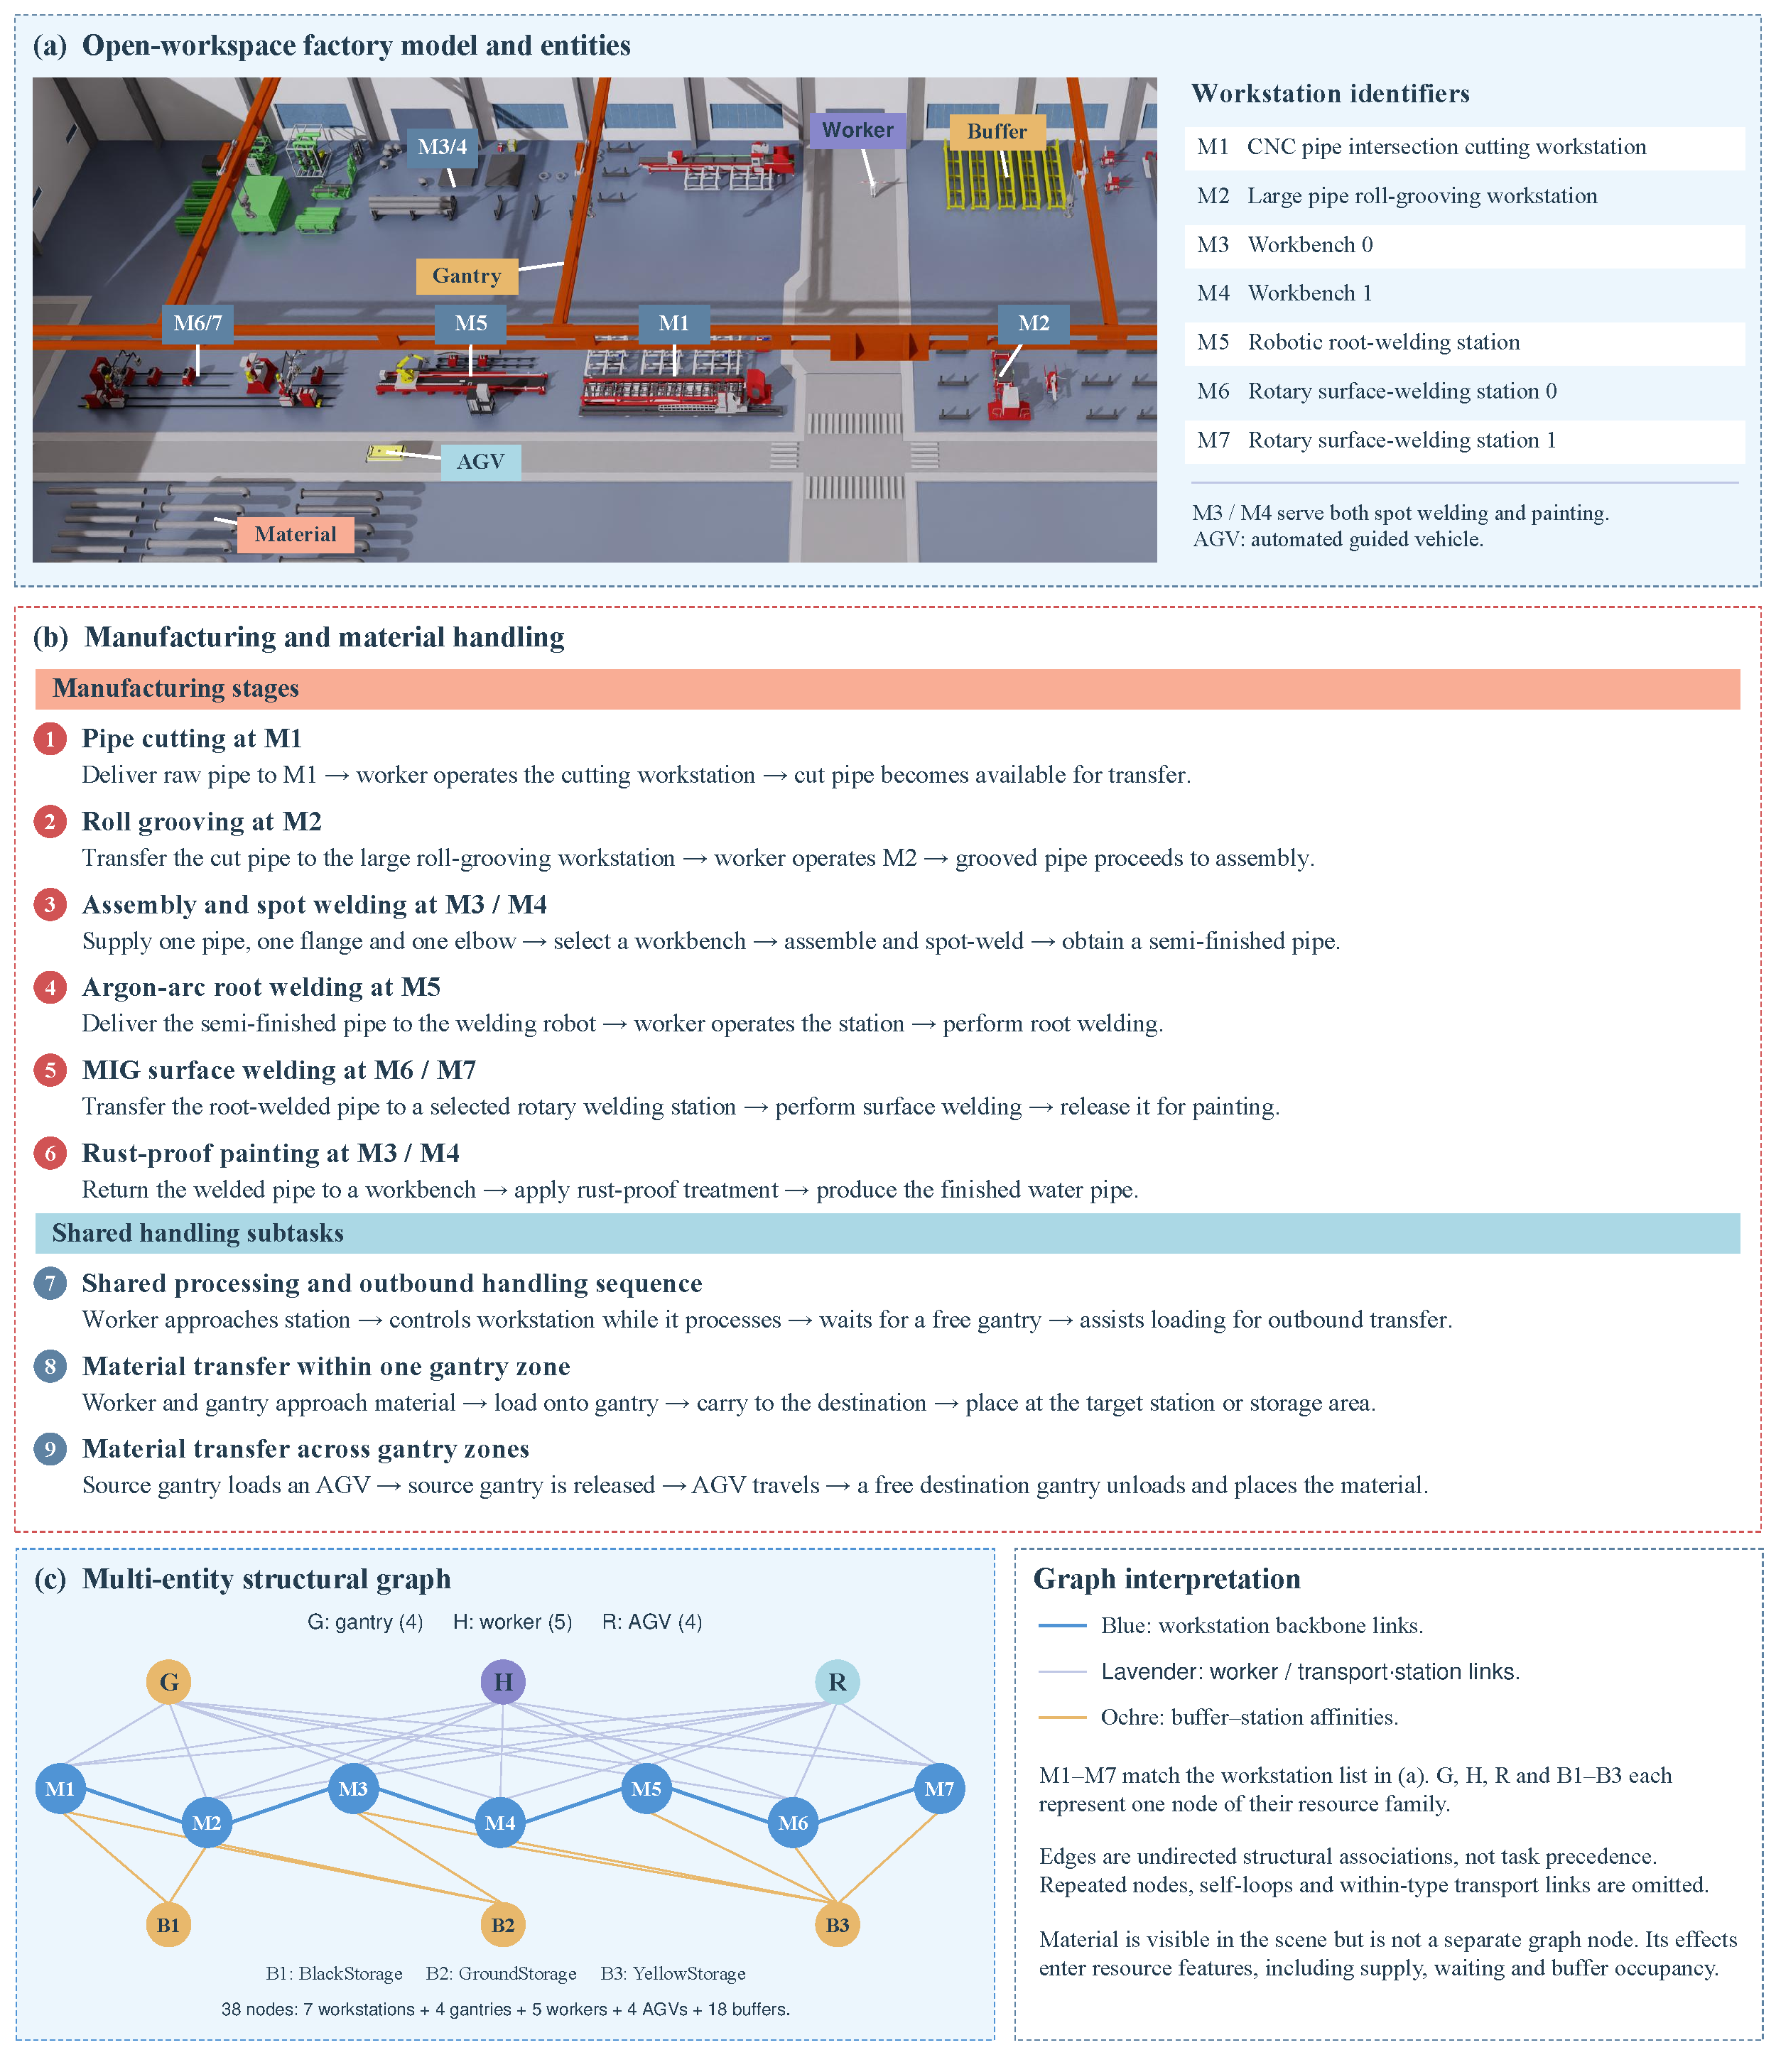
\includegraphics[width=\linewidth]{figures/fig_experiment.pdf}
\caption{Open-workspace factory model developed for NVIDIA Isaac Sim: (a)~resource entities; (b)~manufacturing stages; (c)~structural graph of 38 resources.}
\label{fig:experiment}
\end{figure}

The data-generation environment exposes four operating variation dimensions and applies variations in each dimension at three intervention levels (Table~\ref{tab:disturbance-design}). Level~0 changes episode-wide resource capacity before each model run, Level~1 perturbs sampled processing or service behaviour, and Level~2 injects temporary events during production. The platform supports intensity $I\in\{1,2,3\}$; slash-separated values in the table follow this order. The main \texttt{dense\_i1} collection activates one dimension at a time at $I=1$, while nominal runs keep all dimensions inactive. The injected dimension controls data generation but is not used as the bottleneck or process-cause label.

\begin{table}[!htbp]
\centering
\caption{Four operating variation dimensions and their three intervention levels. Values separated by slashes correspond to $I=1/2/3$. One model step equals one logical second.}
\label{tab:disturbance-design}
\footnotesize
\setlength{\tabcolsep}{3.2pt}
\renewcommand{\arraystretch}{1.12}
\begin{tabularx}{\linewidth}{@{}p{0.13\linewidth}YYY@{}}
\toprule
Dimension & L0: episode configuration & L1: sampled process variation & L2: temporary runtime events \\
\midrule
Workstation & Disable workbench ws1 and rotary-welding ws1 & Processing-time noise $5/10/15$ steps; success rate $0.88/0.76/0.64$; tool wear $15/30/45$ steps per 1,000 steps & $2/(2$--$3)/(3$--$4)$ idle-station failures; additional $1$--$2/2$--$3/3$--$4$ weld or kitting quality-hold windows \\
Worker & Reduce the number of workers from 5 to $3/2/1$ & Service-time scale $1.55/2.10/2.65$; worker-specific skill range $0.8$--$1.4/0.7$--$1.6/0.6$--$1.8$; time noise $12/22/32$ steps & $2/(2$--$3)/(3$--$4)$ temporary absences, applied only when the selected worker is idle \\
Logistics & Reduce the number of AGVs from 4 to $2/1/1$; retain all four zone gantries & Gantry-time scale $1.65/2.30/2.95$ with motion noise $10/18/26$ steps; weak background process variation & $2/(2$--$3)/(3$--$4)$ gantry or AGV freezes; at least one pulse targets an AGV while other vehicles remain active \\
Material & Keep the nominal inventory of ten pipes, flanges, and elbows; no permanent deletion & At steps 400--1,000, temporarily hide $6$--$7/7$--$8/7$--$8$ idle flanges or elbows for $1{,}400$--$2{,}200/2{,}000$--$2{,}700/2{,}500$--$3{,}200$ steps & After the opening shortage, inject $1$--$2/2$--$3/3$--$4$ complementary flange/elbow shortage pulses; pipe blanks are never hidden \\
\bottomrule
\end{tabularx}
\end{table}

For workstation, worker, and logistics operating variations, every Level~2 pulse lasts at least 600 steps and the intensity-specific upper bounds are 900/1,300/1,400 steps. Event targets, start times, counts, and durations are resampled for each episode using a deterministic seed. Adjacent pulses are separated by at least 360 steps, and an event is delayed until an eligible target is idle rather than interrupting an active operation. These controls produce sustained operating variations while avoiding a deterministic one-to-one mapping between an injection and a labelled bottleneck.

A run-stratified, episode-level split gives 140/28/36 training/validation/test episodes from 204 valid episodes, yielding 20,826/4,331/5,354 forecast windows (Table~\ref{tab:exp-dataset}). Preprocessing uses synchronized episode logs; normalization and temporal-pattern prototypes are fitted on the training split only. Invalid episodes affected by the known simulator deadlock are excluded. All comparisons use the same test-window identities, history length, future grid, target resources, and label definitions. Table~\ref{tab:dataset-labels} reports test-label composition. All single-device trajectory comparisons and the case study use the same cutting workstation (\texttt{num02}) from the same test episode; the selection procedure is documented in Appendix~\ref{app:case-details}.

Process-informed labels combine resource-specific operational evidence, filter short runs, and fill one-window internal gaps. At inference, the model uses the observed history rather than retrospective future occupancy. The onset limit is the maximum admissible offset of a newly emerging bottleneck; experiments compare limits of 5, 10, and 15~min. Bottleneck events are required to persist for at least 8~min ($m=8$ one-minute windows), with ongoing events evaluated over their remaining duration. The future label grid remains fixed at 30 windows. Strict report matching uses a three-window onset tolerance; timing errors are reported in minutes. In the label summary below, Upcoming denotes a newly emerging event, Ongoing denotes an event already active at the forecast origin, and No-event denotes a pair with no eligible event.

\begin{table}[!htbp]
\centering
\caption{Dataset and label protocol used in the experiments.}
\label{tab:exp-dataset}
\footnotesize
\setlength{\tabcolsep}{4pt}
\renewcommand{\arraystretch}{1.08}
\begin{tabularx}{\linewidth}{@{}>{\raggedright\arraybackslash}p{\dimexpr 0.30\linewidth + 1cm\relax}@{\hspace{0.03\linewidth}}>{\raggedright\arraybackslash}X@{}}
\toprule
Item & Setting \\
\midrule
Dataset & \texttt{dense\_i1}, 204 valid episodes, 38 resources \\
Split & 140/28/36 episodes; 20,826/4,331/5,354 windows \\
Windowing & 60-s windows; 30 historical + 30 future windows \\
Targets & 15 resources: 7 workstations, 4 gantries, 4 robots \\
Onset limit & $5/10/15$~min \\
Report matching & Three-window onset tolerance \\
\bottomrule
\end{tabularx}
\end{table}

\begin{table}[!htbp]
\centering
\caption{Test-set label composition by onset limit. Counts are window--resource pairs over 5,354 windows $\times$ 15 targets; percentages are shares of all pairs.}
\label{tab:dataset-labels}
\footnotesize
\setlength{\tabcolsep}{3.2pt}
\renewcommand{\arraystretch}{1.08}
\begin{tabularx}{\linewidth}{@{}>{\raggedright\arraybackslash}p{0.24\linewidth}>{\raggedleft\arraybackslash}X>{\raggedleft\arraybackslash}X>{\raggedleft\arraybackslash}X@{}}
\toprule
Onset limit & Upcoming & Ongoing & No-event \\
\midrule
$\leq5$ & 336 (0.42\%) & 766 (0.95\%) & 79,208 (98.63\%) \\
$\leq10$ & 604 (0.75\%) & 768 (0.96\%) & 78,938 (98.29\%) \\
$\leq15$ & 708 (0.88\%) & 770 (0.96\%) & 78,832 (98.16\%) \\
\bottomrule
\end{tabularx}
\end{table}

\subsection{Baseline methods}

Four baselines represent recurrent, graph-based, and Transformer forecasting approaches. LSTM models historical sequences; BSTAN combines graph attention with GRU for blockage/starvation-related prediction~\citep{lai2023bstan}; BTGCN combines production-task graphs with GCN and GRU~\citep{yin2025btgcn}; and PDFormer is adapted from its propagation-delay-aware Transformer architecture for bottleneck prediction~\citep{jiang2023pdformer}. All baselines follow the unified experimental protocol, with architecture-specific input representations and learning algorithms. The validation-only fallback rule is documented in Appendix~\ref{app:additional}.

\begin{table}[!htbp]
\centering
\caption{Baseline models and their roles in the comparison.}
\label{tab:exp-baselines}
\footnotesize
\setlength{\tabcolsep}{4pt}
\renewcommand{\arraystretch}{1.10}
\begin{tabularx}{\columnwidth}{@{}lXX@{}}
\toprule
Model & Core framework & Comparison role \\
\midrule
LSTM & Long short-term memory & Recurrent temporal predictor \\
BSTAN & Graph attention + GRU & Graph-attention predictor \\
BTGCN & Graph convolution + GRU & Graph-convolutional predictor \\
PDFormer & Propagation-delay-aware Transformer & Spatiotemporal Transformer predictor \\
\bottomrule
\end{tabularx}
\end{table}

\subsection{Overall experimental settings and metrics}

All experiments use common data splits, forecast windows, targets, initialization controls, training-budget standards, and validation-based selection. Full and ablation models start from the same fixed parameter state; all selected models and report thresholds are frozen before testing.

Shared PHGST-DM settings appear in Table~\ref{tab:shared-training-protocol}. Training uses AdamW with a batch size of 16, a learning rate of $5\times10^{-5}$, a weight decay of $0.05$, cosine learning-rate decay to $10^{-6}$, and fourfold positive-window oversampling. Under the two-stage training procedure, stage~1 starts from the fixed parameter state shared by all ablation arms, unfreezes all five encoder blocks, and runs for at most 50 epochs with an early-stopping patience of 40. Far-onset weighting doubles onset loss beyond 5~min and uses positive weights $9/10/11$ for the three limits; ordinary and hard false-positive weights are $2.5$ and $2.2$. Stage~2 runs for at most 20 epochs, with the checkpoint selected by validation loss. All runs use seed 42 and provide point estimates rather than multi-seed stability estimates. Appendix~\ref{app:additional} provides loss weights, label thresholds, and decoding details.

The model and report threshold are selected on the validation split. Candidate thresholds are listed explicitly in Table~\ref{tab:shared-training-protocol}; selection uses the internal station-identification F1 among candidates satisfying validation report precision $\geq0.80$ and recall $\geq0.70$. This selection score is not reported as a result; the reported event metric is the onset-qualified F1-score defined below. PHGST-DM uses the selected threshold of $0.94$ for testing at all three onset limits.

For resource $n$ at forecast origin $t$, let $\hat s_{t,n}$ and $s_{t,n}$ denote the predicted and reference onset offsets in minutes. A strict report-level hit requires the correct resource and an absolute onset error within tolerance $\epsilon_s$:
\begin{equation}
|\hat{s}_{t,n}-s_{t,n}|\leq\epsilon_s,\qquad
\epsilon_s=3~\mathrm{min}.
\end{equation}
At the one-minute window resolution, this tolerance equals three windows.

Metrics cover bottleneck-event prediction, process-cause classification, and remaining order time. The reported bottleneck-event F1-score requires both correct station identification and an onset error within three windows. Upcoming recall uses future-event window--resource pairs whose final historical window is non-bottleneck; Ongoing recall uses pairs with an active final historical window. Mean absolute error (MAE) for onset and duration is measured on correctly detected events, while union duration MAE and root mean squared error (RMSE) include missed events and false positives. Event F1 is the harmonic mean of precision and recall; macro recall is the unweighted mean of class-specific recalls. Next-window and 30-window State F1 describe the predicted occupancy over time, including recovery. Process-cause evaluation uses accuracy and macro recall over the four supported classes. Order-completion evaluation uses remaining-time MAE at the line level.

\begin{table}[!htbp]
\centering
\caption{Metrics used in the main evaluation and component analyses.}
\label{tab:exp-metrics}
\footnotesize
\setlength{\tabcolsep}{3.5pt}
\renewcommand{\arraystretch}{1.08}
\begin{tabularx}{\linewidth}{@{}p{0.14\linewidth}p{0.27\linewidth}Y@{}}
\toprule
Group & Metric & Interpretation \\
\midrule
Event & F1-score & Correct station and onset within three windows \\
Warning & Upcoming / ongoing recall & Historically cold / already active resource \\
State & F1 (1 step / horizon) & Occupancy at the next window / across 30 windows \\
Temporal & Onset / duration MAE & Error on correctly detected events \\
Temporal & Union duration MAE/RMSE & Includes missed events and false positives \\
Auxiliary & Remaining-time MAE & Global order-progress error \\
Auxiliary & Cause accuracy / macro recall & Four supported process-cause classes \\
\bottomrule
\end{tabularx}
\end{table}

\FloatBarrier
\section{Overall bottleneck prediction performance}\label{sec:comparison-overview}

This section evaluates how well PHGST-DM jointly predicts bottleneck events, process causes, and remaining order time. Its performance is compared with four baselines under the shared experimental protocol (Tables~\ref{tab:comparison-main}--\ref{tab:comparison-remain}).

\subsection{Bottleneck station, onset, and duration}\label{sec:comparison-event}

At the event level, we assess how accurately PHGST-DM identifies bottleneck stations and predicts their onset, duration, and future occupancy (Table~\ref{tab:comparison-main}).

PHGST-DM achieves the highest event F1, upcoming recall, ongoing recall, and state F1 across the onset limits. Relative to the strongest baseline for each metric and limit, event F1 improves by 8.2--22.1 percentage points and upcoming recall by 28.7--39.9 percentage points. These gains show improved detection before bottlenecks become active, alongside continued coverage of persistent constraints (Figure~\ref{fig:baseline-comparison}).

\begin{table}[!htbp]
\centering
\caption{Bottleneck event and temporal prediction. Scores are percentages except timing MAE (min); best and second-best values are bold and underlined, respectively.}
\label{tab:comparison-main}
\footnotesize
\setlength{\tabcolsep}{3.2pt}
\renewcommand{\arraystretch}{1.12}
\begin{fittable}
\begin{tabular*}{\linewidth}{@{\extracolsep{\fill}}lrrrrrrr@{}}
\toprule
Model & \multicolumn{1}{c}{Event F1 $\uparrow$} & \multicolumn{2}{c}{Event recall $\uparrow$} & \multicolumn{2}{c}{Timing MAE $\downarrow$} & \multicolumn{2}{c}{State F1 $\uparrow$} \\
\cmidrule(lr){2-2}\cmidrule(lr){3-4}\cmidrule(lr){5-6}\cmidrule(l){7-8}
 & F1-score & Upcoming & Ongoing & Onset & Duration & 1 step & 30 steps \\
\midrule
\multicolumn{8}{l}{\textit{Onset limit $\leq5$}} \\
PHGST-DM & \textbf{80.4\%} & \textbf{54.2\%} & \textbf{93.7\%} & 0.127 & \textbf{1.863} & \textbf{88.3\%} & \textbf{52.5\%} \\
LSTM & 58.3\% & 9.9\% & 68.7\% & 0.056 & 3.855 & 29.5\% & 29.5\% \\
BSTAN & 68.7\% & 9.5\% & 79.4\% & 0.043 & 3.565 & 71.9\% & \underline{37.9\%} \\
BTGCN & 66.9\% & 4.6\% & 78.6\% & \underline{0.020} & 3.322 & 64.3\% & 37.2\% \\
PDFormer & \underline{72.2\%} & \underline{14.3\%} & \underline{89.2\%} & \textbf{0.008} & \underline{2.725} & \underline{85.4\%} & 34.7\% \\
\midrule
\multicolumn{8}{l}{\textit{Onset limit $\leq10$}} \\
PHGST-DM & \textbf{77.8\%} & \textbf{53.5\%} & \textbf{93.9\%} & 0.227 & \textbf{1.788} & \textbf{89.2\%} & \textbf{58.9\%} \\
LSTM & 47.7\% & 11.2\% & 69.3\% & 0.388 & 3.768 & 27.5\% & 26.2\% \\
BSTAN & \underline{60.9\%} & 5.7\% & 79.6\% & \underline{0.153} & 3.533 & 63.2\% & \underline{36.5\%} \\
BTGCN & 57.9\% & 4.5\% & 72.2\% & \textbf{0.117} & 3.238 & 56.6\% & 35.9\% \\
PDFormer & 59.8\% & \underline{22.2\%} & \underline{90.2\%} & 0.203 & \underline{2.798} & \underline{84.2\%} & 34.7\% \\
\midrule
\multicolumn{8}{l}{\textit{Onset limit $\leq15$}} \\
PHGST-DM & \textbf{76.8\%} & \textbf{53.7\%} & \textbf{93.0\%} & \underline{0.227} & \textbf{1.716} & \textbf{90.0\%} & \textbf{61.0\%} \\
LSTM & 46.1\% & 10.2\% & 64.3\% & 0.453 & 3.615 & 26.8\% & 26.0\% \\
BSTAN & 53.4\% & 4.4\% & 70.0\% & \textbf{0.222} & 3.422 & 59.3\% & 33.5\% \\
BTGCN & 51.8\% & 5.4\% & 69.9\% & 0.302 & 3.121 & 46.1\% & 32.3\% \\
PDFormer & \underline{54.7\%} & \underline{25.0\%} & \underline{89.5\%} & 0.499 & \underline{2.744} & \underline{82.2\%} & \underline{36.0\%} \\
\bottomrule
\end{tabular*}
\end{fittable}
\end{table}

Detected-event duration MAE is 0.86--1.03~min lower than that of the best baseline at each onset limit, a relative reduction of 31.6--37.5\%. This extends the benefit from identifying an affected station to estimating how long its constraint persists. Timing MAE is conditional on correct detection, and onset MAE alone does not show a uniform advantage over the baselines. Further onset-distance and resource-type results appear in Appendix~\ref{app:supplementary-results}.

\begin{figure}[!htbp]
\centering
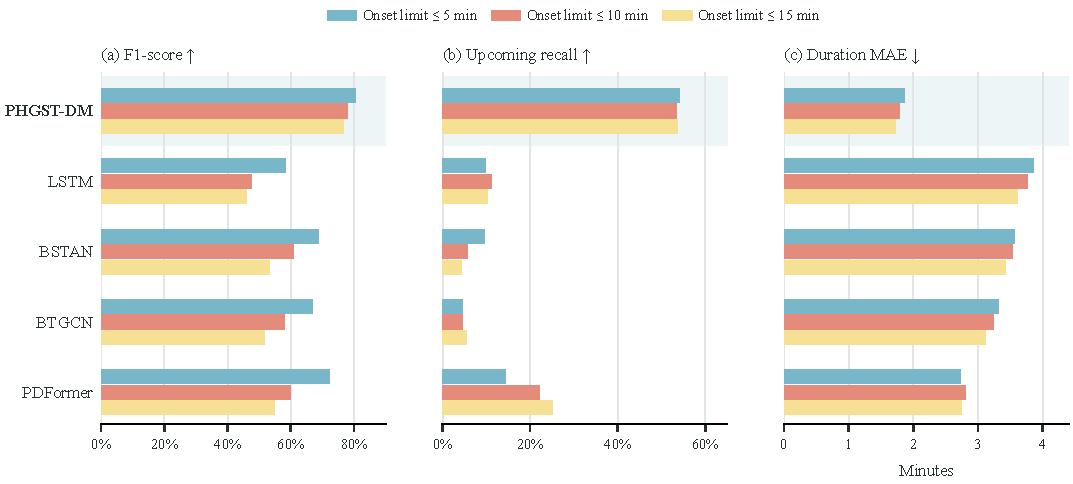
\includegraphics[width=0.96\textwidth,height=0.66\textheight,keepaspectratio]{figures/fig_range_response.pdf}
\caption{Grouped comparison of (a)~F1-score, (b)~Upcoming recall, and (c)~detected-event duration MAE across onset limits.}
\label{fig:baseline-comparison}
\end{figure}

\begin{figure}[!htbp]
\centering
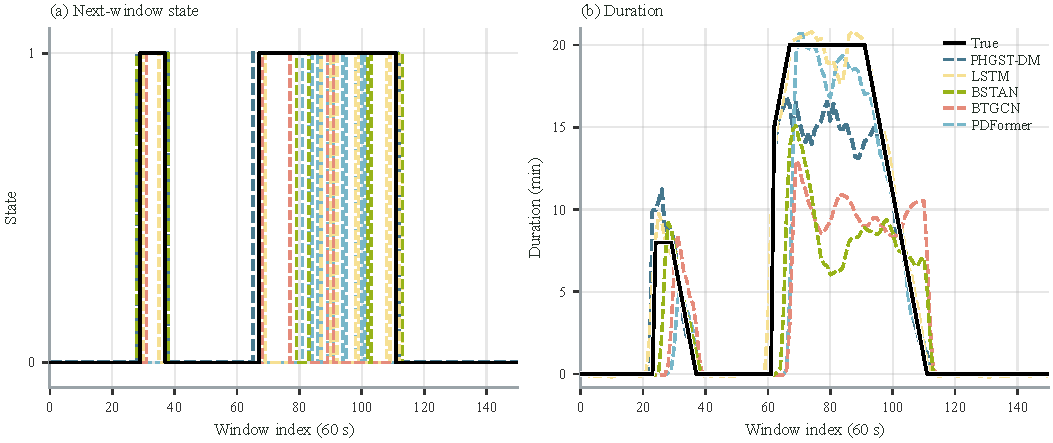
\includegraphics[width=0.90\textwidth,height=0.66\textheight,keepaspectratio]{figures/key_device_models_aligned.pdf}
\caption{Comparison of PHGST-DM and baselines at Onset limit~$\leq5$: (a)~next-window state; (b)~duration with the true reference truncated at 20~min for visualization (black: ground truth; dashed: predictions).}
\label{fig:key-device-baselines}
\end{figure}

Figure~\ref{fig:key-device-baselines} shows the corresponding trajectories. PHGST-DM tracks both bottleneck intervals and the subsequent recovery, connecting event coverage to successive duration forecasts. The displayed true-duration reference is truncated at 20~min, while every model retains the 30-min prediction horizon.

\subsection{Bottleneck process-cause prediction}\label{sec:comparison-cause}

The process-cause comparison covers four operational conditions: material shortage, transport delay, queue buildup, and downstream blockage (Table~\ref{tab:comparison-state}).

PHGST-DM outperforms the four baselines in both cause accuracy and macro recall across the onset limits. Compared with the strongest baseline at each limit, macro recall improves by 1.4--4.3 percentage points.

\begin{table}[!htbp]
\centering
\caption{Bottleneck process-cause prediction (\%). Best and second-best values are bold and underlined, respectively.}
\label{tab:comparison-state}
\footnotesize
\setlength{\tabcolsep}{3.2pt}
\renewcommand{\arraystretch}{1.12}
\begin{fittable}
\begin{tabular*}{\linewidth}{@{\extracolsep{\fill}}lrrrrrr@{}}
\toprule
Model & \multicolumn{2}{c}{Onset limit $\leq5$} & \multicolumn{2}{c}{Onset limit $\leq10$} & \multicolumn{2}{c}{Onset limit $\leq15$} \\
\cmidrule(lr){2-3}\cmidrule(lr){4-5}\cmidrule(l){6-7}
 & Accuracy $\uparrow$ & Macro R $\uparrow$ & Accuracy $\uparrow$ & Macro R $\uparrow$ & Accuracy $\uparrow$ & Macro R $\uparrow$ \\
\midrule
PHGST-DM & \textbf{96.5\%} & \textbf{96.7\%} & \textbf{96.2\%} & \textbf{96.5\%} & \textbf{97.4\%} & \textbf{97.8\%} \\
LSTM & 93.8\% & 92.0\% & 93.6\% & 93.0\% & 94.4\% & 92.2\% \\
BSTAN & \underline{95.7\%} & \underline{95.2\%} & \underline{95.9\%} & \underline{95.1\%} & \underline{95.1\%} & \underline{93.5\%} \\
BTGCN & 90.0\% & 88.2\% & 90.7\% & 90.0\% & 90.7\% & 90.0\% \\
PDFormer & 88.8\% & 88.7\% & 76.9\% & 74.7\% & 79.6\% & 77.3\% \\
\bottomrule
\end{tabular*}
\end{fittable}
\end{table}

\subsection{Order-completion remaining-time prediction}\label{sec:comparison-remain}

After joint training, the remaining-time head is fine-tuned while the encoder and all other prediction heads remain fixed. Table~\ref{tab:comparison-remain} compares the first- and second-stage PHGST-DM predictions with the baselines on the same test windows.

\begin{table}[!htbp]
\centering
\caption{Global order remaining-time MAE (min; lower is better). Best and second-best values are bold and underlined, respectively.}
\label{tab:comparison-remain}
\footnotesize
\setlength{\tabcolsep}{3pt}
\renewcommand{\arraystretch}{1.10}
\begin{fittable}
\begin{tabular*}{\linewidth}{@{\extracolsep{\fill}}lrrr@{}}
\toprule
Model & Onset limit $\leq5$ & Onset limit $\leq10$ & Onset limit $\leq15$ \\
\midrule
PHGST-DM (stage 1) & 10.93 & 11.21 & 9.72 \\
PHGST-DM (stage 2) & \textbf{9.60} & \textbf{9.27} & \textbf{8.91} \\
\midrule
LSTM & 10.59 & \underline{10.61} & \underline{9.01} \\
BSTAN & 14.77 & 13.855 & 13.56 \\
BTGCN & 19.34 & 18.10 & 12.83 \\
PDFormer & \underline{10.437} & 11.254 & 10.422 \\
\bottomrule
\end{tabular*}
\end{fittable}
\end{table}

Second-stage fine-tuning reduces remaining-time MAE by 0.81--1.94~min across the onset limits, equivalent to an 8.3--17.3\% reduction relative to stage~1, while retaining the event and cause outputs.

Figure~\ref{fig:remain-finetune} shows that most of the improvement occurs in the early and middle production phases.

After fine-tuning, PHGST-DM achieves the lowest remaining-time MAE at every onset limit, reducing error by 0.10--1.34~min relative to the strongest baseline at each limit. This combines competitive order-progress estimation with the resource-level event and process-cause forecasts.

\begin{figure}[!htbp]
\centering
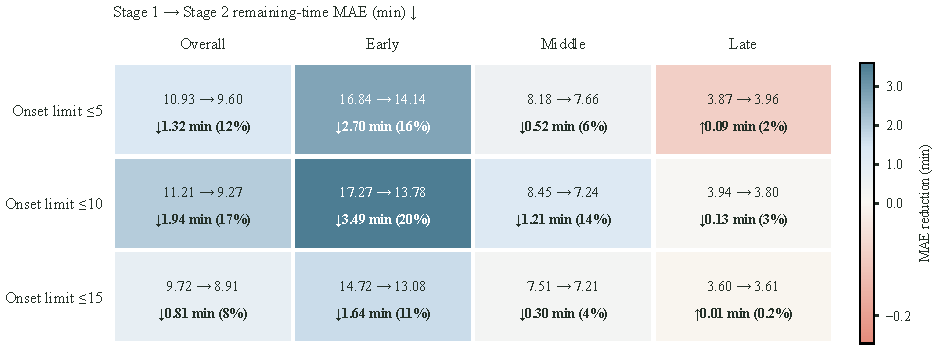
\includegraphics[width=0.90\textwidth,height=0.66\textheight,keepaspectratio]{figures/fig_remain_dumbbell.pdf}
\caption{Effect of remaining-time fine-tuning across early, middle, and late production phases (blue: MAE decrease; coral: increase).}
\label{fig:remain-finetune}
\end{figure}

\FloatBarrier
\section{Evaluation of the proposed components}

The component studies isolate heterogeneous multi-entity representation, process-informed supervision and temporal pattern clustering, and recurrent-pattern-guided delay-aware modelling (Table~\ref{tab:ablation-arms}). Full and all ablation arms share initialization, training budget, curriculum, and validation selection. Remaining-time ablations compare models before head-specific fine-tuning to keep the optimization conditions matched; the fine-tuned full-model results are evaluated in Section~\ref{sec:comparison-remain}. Section~\ref{sec:decoder-training} examines the supporting decoder and training components.

\begin{table}[!htbp]
\centering
\caption{Ablation arms. Every comparison, including the Full reference, begins from identical parameter values and uses the same 50-epoch budget, Onset limit~$\leq5\rightarrow$Onset limit~$\leq10\rightarrow$Onset limit~$\leq15$ curriculum, and validation-controlled model-selection rule.}
\label{tab:ablation-arms}
\footnotesize
\setlength{\tabcolsep}{3.5pt}
\renewcommand{\arraystretch}{1.08}
\begin{tabularx}{\linewidth}{@{}p{0.20\linewidth}p{0.23\linewidth}Y@{}}
\toprule
Arm & Component & Change relative to Full \\
\midrule
NoGraph & Heterogeneous graph & Self-loop adjacency only; no factory edges  \\
NoGroup & Heterogeneous graph & One linear projection of the 27 channels instead of six semantic groups  \\
NoCross & Heterogeneous graph & Within-type edges only; cross-type semantic attention masked  \\
NoInfo & Heterogeneous graph & Only workstations observed; non-workstation features and five coupling channels zeroed  \\
WorkstationOnly & Heterogeneous graph & NoCross and NoInfo combined  \\
NoCluster & Temporal pattern clustering & Temporal pattern clustering removed  \\
NoPattern & \makecell[l]{Delay-aware modelling} & Recent-patch matching to the temporal-pattern prototype bank disabled  \\
NoSplit & Decoder & One shared event-occurrence head for continuing and new events  \\
NoFarBoost & Training & Far-onset weighting and enhanced false-alarm penalty removed  \\
\bottomrule
\end{tabularx}
\end{table}

\subsection{Heterogeneous multi-entity representation}\label{sec:entity-analysis}

Multi-entity ablations assess the contribution of non-workstation observations and cross-resource relations to advance warning. The ablations restrict non-workstation information, cross-type relations, factory edges, or grouped embedding while retaining the same targets (Tables~\ref{tab:ablation-arms} and~\ref{tab:entity-ablation-new}).

\begin{table}[!htbp]
\centering
\caption{Heterogeneous-graph and multi-entity ablation results. Dur. MAE is union error (min); best and second-best values are bold and underlined.}
\label{tab:entity-ablation-new}
\footnotesize
\setlength{\tabcolsep}{3.5pt}
\renewcommand{\arraystretch}{1.05}
\begin{fittable}
\begin{tabular*}{\linewidth}{@{\extracolsep{\fill}}llrrrrr@{}}
\toprule
Arm & \makecell{Onset\\limit} & F1-score & \makecell{Upcoming\\R} & \makecell{Type\\hmean} & \makecell{State F1\\(1 step)} & Dur.\ MAE \\
\midrule
Full & $\leq5$ & \textbf{80.4\%} & \textbf{54.2\%} & \textbf{50.5\%} & \textbf{88.3\%} & \textbf{4.17} \\
NoGraph &  & 74.6\% & 10.4\% & 38.4\% & \underline{87.3\%} & 5.48 \\
NoGroup &  & \underline{75.3\%} & \underline{33.3\%} & \underline{43.2\%} & 83.5\% & \underline{5.11} \\
NoCross &  & 71.6\% & 22.0\% & 39.6\% & 81.2\% & 5.28 \\
NoInfo &  & 64.4\% & 4.9\% & 0.0\% & 69.9\% & 6.66 \\
WorkstationOnly &  & 65.0\% & 3.3\% & 0.0\% & 70.9\% & 6.51 \\
\midrule
Full & $\leq10$ & \textbf{77.8\%} & \textbf{53.5\%} & \textbf{53.0\%} & \textbf{89.2\%} & \textbf{4.38} \\
NoGraph &  & 64.9\% & 6.5\% & 37.6\% & \underline{84.4\%} & 6.46 \\
NoGroup &  & \underline{65.1\%} & \underline{48.5\%} & \underline{45.2\%} & 82.6\% & \underline{6.05} \\
NoCross &  & 57.1\% & 20.7\% & 37.1\% & 75.9\% & 6.60 \\
NoInfo &  & 54.4\% & 2.1\% & 0.0\% & 68.4\% & 7.57 \\
WorkstationOnly &  & 55.9\% & 1.4\% & 0.0\% & 70.8\% & 7.40 \\
\midrule
Full & $\leq15$ & \textbf{76.8\%} & \textbf{53.7\%} & \textbf{53.6\%} & \textbf{90.0\%} & \textbf{4.43} \\
NoGraph &  & \underline{61.2\%} & 3.7\% & 36.0\% & \underline{86.5\%} & 6.57 \\
NoGroup &  & 60.4\% & \underline{43.2\%} & \underline{46.9\%} & 81.9\% & \underline{6.34} \\
NoCross &  & 51.4\% & 31.1\% & 36.5\% & 76.0\% & 6.77 \\
NoInfo &  & 44.1\% & 21.8\% & 0.0\% & 59.6\% & 7.66 \\
WorkstationOnly &  & 53.4\% & 2.1\% & 0.0\% & 70.6\% & 7.46 \\
\bottomrule
\end{tabular*}
\end{fittable}
\end{table}

At Onset limit~$\leq5$, the full representation improves upcoming recall by 50.9 percentage points over WorkstationOnly and by 49.3 points over NoInfo. Removing cross-resource relations or factory edges also weakens distant-event warning (Figure~\ref{fig:cross-resource-evidence}). These comparisons support both the broader observation scope and its relational organization for recognizing constraints that workstation-centred inputs alone fail to reveal.

\begin{figure}[htbp]
\centering
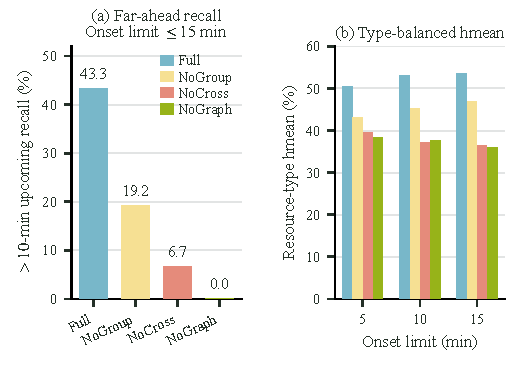
\includegraphics[width=0.82\columnwidth]{figures/fig_cross_resource_evidence.pdf}
\caption{Cross-resource evidence from structural ablations: (a)~far-onset report recall at Onset limit~$\leq15$; (b)~type-hmean F1 across onset limits.}
\label{fig:cross-resource-evidence}
\end{figure}

The complete representation also tracks bottleneck persistence and recovery more closely in Figure~\ref{fig:key-device-entity}. Thus, the heterogeneous graph benefits both advance warning and duration tracking. Resource-level results appear in Appendix~\ref{app:supplementary-results}, with case selection in Appendix~\ref{app:case-details}.

\begin{figure}[!htbp]
\centering
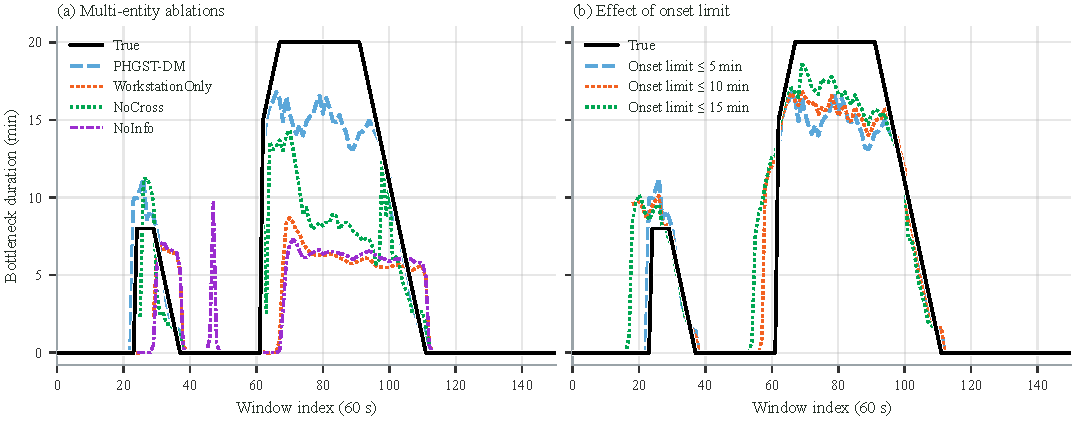
\includegraphics[width=0.96\textwidth,height=0.66\textheight,keepaspectratio]{figures/key_device_entity.pdf}
\caption{Bottleneck-duration traces: panel~(a) compares multi-entity ablations with a 5-min onset limit; panel~(b) compares PHGST-DM with onset limits of 5, 10, and 15~min. The black curve shows the true-duration reference.}
\label{fig:key-device-entity}
\end{figure}

\paragraph*{Cross-resource attention.}\label{sec:attention-protocol}
Figure~\ref{fig:attn-types} examines how the model combines resource information under normal, upcoming, and ongoing bottleneck conditions. Each condition uses 96 episode-stratified test samples, with attention averaged over samples, history steps, heads, and layers. Type-level cells represent mean query-type/attended-type weights. The geographic branch consistently places greater weight on workstations, while the semantic branch exhibits strong workstation--AGV associations and distinct gantry and worker patterns. These associations complement the ablation results by showing how information about production, transport, and workers enters the learned representation. The two branches provide complementary resource views for forecasting constraints whose operational context extends beyond the affected workstation.

\begin{figure}[!htbp]
\centering
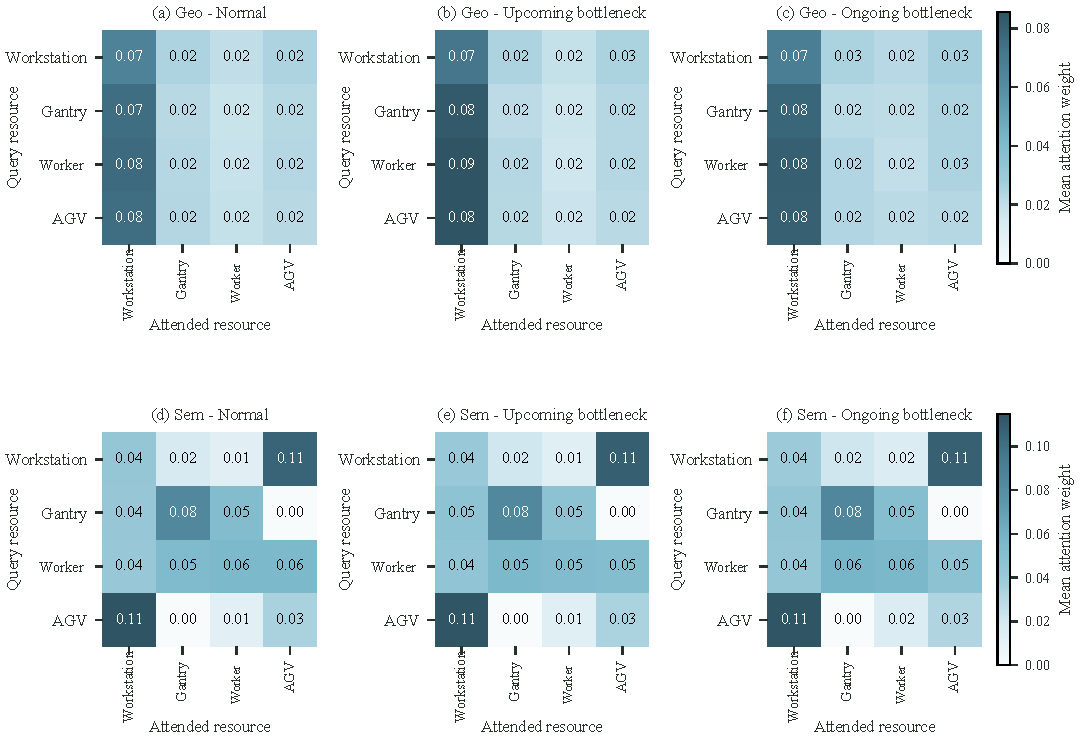
\includegraphics[width=0.92\textwidth,height=0.66\textheight,keepaspectratio]{figures/attention_heatmaps/fig06_entity_type_attention.pdf}
\caption{Type-level attention summary under normal, upcoming, and ongoing conditions (buffers omitted).}
\label{fig:attn-types}
\end{figure}

\subsection{Process-informed supervision and temporal pattern clustering}\label{sec:supervision-analysis}

Three complementary studies address temporal pattern clustering, process-cause supervision, and the production relevance of the constructed event labels.

\paragraph*{(1) Effects of temporal pattern clustering.}
NoCluster tests the predictive value of clustering historical patches into recurrent-pattern prototypes (Table~\ref{tab:group-ablation}); NoPattern separately tests prototype use in Section~\ref{sec:delay-analysis}.

At Onset limit~$\leq15$, temporal pattern clustering improves event F1 by 23.1 percentage points and reduces union duration MAE by 2.22~min relative to NoCluster, a 33.4\% reduction. Gains in upcoming recall and next-window state F1 across the onset limits further show that the pattern bank supports both detection and temporal reconstruction.

\begin{table}[!htbp]
\centering
\caption{Temporal-clustering ablation results. Dur. MAE is union error; Dur. MAE (tp) uses correctly reported events; values are in minutes.}
\label{tab:group-ablation}
\footnotesize
\setlength{\tabcolsep}{3.5pt}
\renewcommand{\arraystretch}{1.08}
\begin{fittable}
\begin{tabular*}{\linewidth}{@{\extracolsep{\fill}}llrrrrr@{}}
\toprule
Arm & \makecell{Onset\\limit} & F1-score & \makecell{Upcoming\\R} & \makecell{State F1\\(1 step)} & Dur.\ MAE & \makecell{Dur. MAE\\(tp)} \\
\midrule
Full & $\leq5$ & \textbf{80.4\%} & \textbf{54.2\%} & \textbf{88.3\%} & \textbf{4.17} & \textbf{1.86} \\
NoCluster & & 73.4\% & 12.5\% & 84.1\% & 5.43 & 2.89 \\
\midrule
Full & $\leq10$ & \textbf{77.8\%} & \textbf{53.5\%} & \textbf{89.2\%} & \textbf{4.38} & \textbf{1.79} \\
NoCluster & & 57.0\% & 34.6\% & 78.9\% & 6.69 & 2.40 \\
\midrule
Full & $\leq15$ & \textbf{76.8\%} & \textbf{53.7\%} & \textbf{90.0\%} & \textbf{4.43} & \textbf{1.72} \\
NoCluster & & 53.7\% & 37.3\% & 81.9\% & 6.65 & 2.30 \\
\bottomrule
\end{tabular*}
\end{fittable}
\end{table}

\paragraph*{(2) Effects of cause supervision.}
The cause-supervision comparison holds labels, data split, onset limit, initialization, seed, and training budget constant (Table~\ref{tab:matched-cause}).

Adding cause supervision improves cause accuracy at the separately selected operating point by 67.0 percentage points and macro recall by 68.2 points, while logged station F1 changes by only 0.2 points.

\begin{table}[!htbp]
\centering
\caption{Matched-budget cause-supervision study at onset limit $\leq5$. Values are percentages.}
\label{tab:matched-cause}
\footnotesize
\setlength{\tabcolsep}{3.5pt}
\renewcommand{\arraystretch}{1.08}
\begin{fittable}
\begin{tabular*}{\linewidth}{@{\extracolsep{\fill}}lrr@{}}
\toprule
Metric & Backbone & +Cause \\
\midrule
Logged station F1 & 73.5\% & 73.3\% \\
Logged cause acc. & 19.5\% & \textbf{89.5\%} \\
Selected cause acc. & 25.2\% & \textbf{92.2\%} \\
Selected cause macro recall & 25.5\% & \textbf{93.7\%} \\
\bottomrule
\end{tabular*}
\end{fittable}
\end{table}

% Evidence: isaac_factory origin/dev_tyx, 8767583f3ed6392cfd8061d4a80de94fcfb9d7a0.
% Source: bottleneck ground-truth validity notes (2026-10-14), checked against label/evaluation code.
% Imported summary values: experiments/data/label_validity_dev_tyx_8767583.json.
\paragraph*{(3) Validation against production sensitivity.}
To assess the production relevance of the event labels, the pilot compares their rankings with order-completion sensitivity under a fixed counterfactual replay protocol. The pilot uses 30 disturbance-free development episodes, separately from predictor training and testing. At a saved factory state, each of seven workstation candidates is accelerated in a separate replay: workstation processing and associated worker-service durations are scaled by $0.8$ (a $1.25\times$ service rate) for 1,200 model steps. Baseline and intervention branches start from the same simulator and random-number states and run to order completion. The reduction in completion time measures production sensitivity. Label methods rank candidates using the preceding three fully observed windows. NDCG@3 measures ranking quality; Positive Recall@$k$ measures top-$k$ coverage; Weighted Recall@3 weights coverage by positive sensitivity; and Coverage@3$_{0.9}$ concerns resources within 90\% of the maximum sensitivity. This fixed acceleration experiment assesses label relevance, not a forecast-guided intervention policy.

\begin{figure}[htbp]
\centering
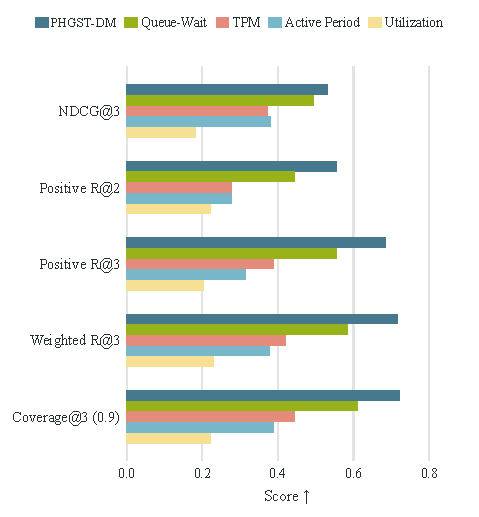
\includegraphics[width=0.76\linewidth,height=0.49\textheight,keepaspectratio]{figures/fig_label_oracle_bars.pdf}
\caption{Counterfactual sensitivity alignment in the exploratory pilot ($\uparrow$: higher is better).}
\label{fig:label-oracle-pilot}
\end{figure}

The process-informed labelling method used by PHGST-DM obtains the highest point estimates on all retained alignment metrics (Figure~\ref{fig:label-oracle-pilot}). Compared with Queue-Wait, NDCG@3 increases by 0.036, Coverage@3$_{0.9}$ improves by 11.1 percentage points, and weighted Recall@3 improves by 13.1 percentage points. Detailed point estimates, reported 95\% confidence intervals for the labelling method, and stage-resolved results are provided in Appendix~\ref{app:supplementary-results}. These exploratory results suggest that combining process evidence helps identify and prioritize resources whose acceleration reduces order-completion time.
\FloatBarrier

\subsection{Delay-aware modelling}\label{sec:delay-analysis}

NoPattern disables recent-patch matching to the fixed prototype bank while retaining the graph and attention branches (Table~\ref{tab:delay-ablation-new}). It isolates historical pattern conditioning from the availability of heterogeneous observations.

At Onset limit~$\leq15$, prototype matching raises strict recall for events more than 10~min ahead by 27.0 percentage points relative to NoPattern, more than doubling distant-event coverage. Improvements in event identification and auxiliary outputs further show that recurrent-pattern conditioning adds forecasting value beyond the heterogeneous graph alone.

This distant-warning benefit supports using earlier resource patterns to anticipate constraints that emerge later, addressing the difficulty of predicting delayed cross-resource effects. Further results appear in Appendix~\ref{app:supplementary-results}.

\begin{table}[!htbp]
\centering
\caption{Temporal-pattern matching ablation in delay-aware modelling. Values compare stage-1 models; onset-distance recall uses strict report matching.}
\label{tab:delay-ablation-new}
\footnotesize
\setlength{\tabcolsep}{2.6pt}
\renewcommand{\arraystretch}{1.08}
\begin{fittable}
\begin{tabular*}{\linewidth}{@{\extracolsep{\fill}}llrrrrrrr@{}}
\toprule
Arm & \makecell{Onset\\limit} & F1-score & \makecell{Upcoming\\R} & $R_{\mathrm{up,rep}}^{6\text{--}10}$ & $R_{\mathrm{up,rep}}^{>10}$ & Queue R & \makecell{Cause\\Macro R} & \makecell{Remain\\MAE} \\
\midrule
Full (stage 1) & $\leq5$ & \textbf{80.4\%} & \textbf{54.2\%} & --- & --- & \textbf{98.4\%} & \textbf{96.7\%} & \textbf{10.93} \\
NoPattern & & 74.5\% & 16.7\% & --- & --- & 14.5\% & 73.4\% & 18.62 \\
\midrule
Full (stage 1) & $\leq10$ & \textbf{77.8\%} & \textbf{53.5\%} & \textbf{46.6\%} & --- & \textbf{98.4\%} & \textbf{96.5\%} & \textbf{11.21} \\
NoPattern & & 58.8\% & 27.8\% & 14.9\% & --- & 47.6\% & 80.5\% & 13.35 \\
\midrule
Full (stage 1) & $\leq15$ & \textbf{76.8\%} & \textbf{53.7\%} & \textbf{52.2\%} & \textbf{43.3\%} & \textbf{98.4\%} & \textbf{97.8\%} & \textbf{9.72} \\
NoPattern & & 60.1\% & 42.7\% & 39.6\% & 16.3\% & 57.3\% & 85.0\% & 11.06 \\
\bottomrule
\end{tabular*}
\end{fittable}
\end{table}

\paragraph*{Historical attention and onset-limit comparisons.}
The descriptive attention maps show that the model draws on multiple historical regions and reweights resource associations across layers and onset limits. The full maps and their interpretation are retained in Appendix~\ref{app:attention-analysis}. These weights describe learned associations and are not evidence of causal effects.

\subsection{Supporting decoder components}\label{sec:decoder-training}

Two decoder-related ablations examine split event heads and far-onset enhancement under the common training and selection protocol (Table~\ref{tab:decoder-ablation}). NoSplit examines the distinction between continuing and newly emerging events; NoFarBoost examines weighting for distant onsets. Each retains its validation-selected operating point.

\begin{table}[!htbp]
\centering
\caption{Split event-head and far-onset ablation results. Thr is the validation-selected threshold; Dur. MAE is union duration error (min).}
\label{tab:decoder-ablation}
\footnotesize
\setlength{\tabcolsep}{3.5pt}
\renewcommand{\arraystretch}{1.08}
\begin{fittable}
\begin{tabular*}{\linewidth}{@{\extracolsep{\fill}}llrrrrrr@{}}
\toprule
Arm & \makecell{Onset\\limit} & Thr & F1-score & \makecell{Upcoming\\R} & $R_{\mathrm{up,rep}}^{>10}$ & \makecell{Ongoing\\R} & Dur.\ MAE \\
\midrule
Full & $\leq5$ & 94.0\% & 80.4\% & 54.2\% & --- & \textbf{93.7\%} & 4.17 \\
NoFarBoost & & 90.0\% & \textbf{81.9\%} & \textbf{54.5\%} & --- & 92.3\% & \textbf{4.03} \\
NoSplit & & 94.0\% & 72.7\% & 19.0\% & --- & 93.5\% & 5.56 \\
\midrule
Full & $\leq10$ & 94.0\% & \textbf{77.8\%} & 53.5\% & --- & 93.9\% & \textbf{4.38} \\
NoFarBoost & & 88.0\% & 75.2\% & \textbf{56.0\%} & --- & 92.3\% & 4.66 \\
NoSplit & & 94.0\% & 58.0\% & 24.7\% & --- & \textbf{94.7\%} & 6.63 \\
\midrule
Full & $\leq15$ & 94.0\% & \textbf{76.8\%} & \textbf{53.7\%} & \textbf{43.3\%} & 93.0\% & \textbf{4.43} \\
NoFarBoost & & 94.0\% & 74.1\% & 48.9\% & 24.0\% & 92.5\% & 4.87 \\
NoSplit & & 94.0\% & 58.6\% & 35.3\% & 12.5\% & \textbf{95.1\%} & 6.36 \\
\bottomrule
\end{tabular*}
\end{fittable}
\end{table}

At Onset limit~$\leq5$, split event heads improve upcoming recall by 35.2 percentage points over NoSplit while retaining high ongoing recall. At Onset limit~$\leq15$, far-onset enhancement raises strict recall beyond 10~min by 19.3 points over NoFarBoost. These gains connect the decoder designs to recognizing newly emerging and more distant events.

Figure~\ref{fig:key-device-struct-graph} shows closer duration tracking by the complete model, with stronger underestimation or post-event spikes in the ablations. Together, the comparisons support decoding that distinguishes current persistence from future onset; weighting benefits remain range-dependent, with NoFarBoost performing better at Onset limit~$\leq5$.

\begin{figure}[!htbp]
\centering
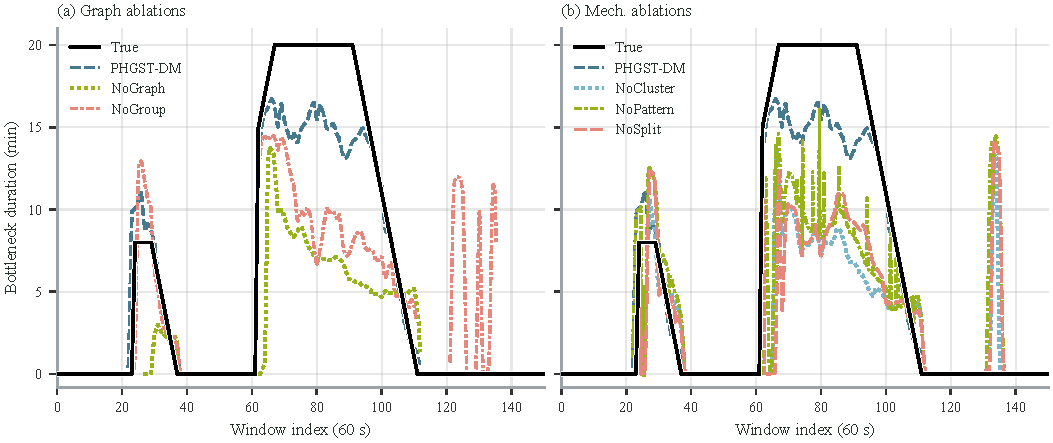
\includegraphics[width=0.96\textwidth,height=0.66\textheight,keepaspectratio]{figures/key_device_struct_pair.pdf}
\caption{Ablation traces (Onset limit~$\leq5$): (a)~graph arms; (b)~process-rule/context, delay-aware modelling, and decoder arms.}
\label{fig:key-device-struct-graph}
\end{figure}

\FloatBarrier
\section{Case study}\label{sec:case-study}

Moving from aggregate results to individual workstation trajectories, the case study assesses predictions of bottleneck onset, duration, and next-window occupancy. The selected episode contains an approximately 8-min bottleneck and a 49-min bottleneck. The prediction horizon is 30~min; the plotted true-duration reference is truncated at 20~min for readability (Figure~\ref{fig:key-device-baselines}). The case is selected by first retaining devices with at least the median event count, then choosing the device with the most events in a single episode, with PHGST-DM one-step F1 breaking ties. Its episode is selected by the number and length of bottleneck segments.

PHGST-DM warns approximately 1~min before the short event, maintains coverage through both intervals, and follows the predicted-duration decline towards recovery. Relative to the baselines, its trajectory contains fewer coverage gaps and follows the sustained constraint more closely (Figure~\ref{fig:key-device-baselines}). Successive forecasts therefore describe bottleneck development through onset, persistence, and recovery.

The workstation state map shows coverage across resources in the same episode (Figure~\ref{fig:all-devices-main}). Full covers the positive cells of both the cutting and second welding workstations, improving episode State F1 by 4.0 percentage points over the strongest ablated configuration, NoGraph. NoInfo and NoCluster miss the welding interval, while NoGraph fragments it. The full model therefore preserves a more complete view of simultaneous workstation constraints within the episode.

% Allow the final experimental figures and Discussion to flow across columns.
\begin{figure}[!htbp]
\centering
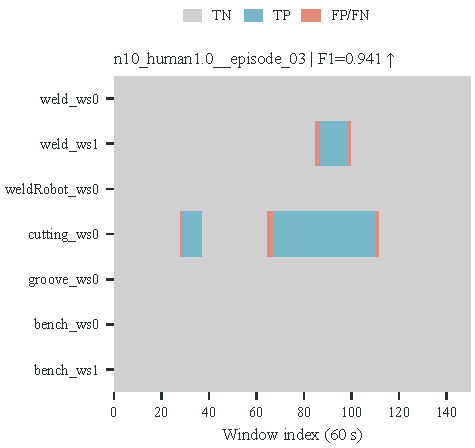
\includegraphics[width=0.82\columnwidth,height=0.66\textheight,keepaspectratio]{figures/all_devices_state_main.pdf}
\caption{Next-window state map for seven workstation targets (grey: TN; light blue: TP; coral: FP/FN). TN, TP, FP, and FN denote true negatives, true positives, false positives, and false negatives, respectively.}
\label{fig:all-devices-main}

\end{figure}



\paragraph*{Resource-level coverage.}
Figure~\ref{fig:per-device} examines whether the joint predictor covers workstations, gantries, and AGVs on the full Onset limit~$\leq5$ test split. Reporting event F1 alongside union duration error separates recognition of an affected resource from reconstruction of its bottleneck interval. The results extend the coverage assessment across resource families and make device-level variation visible instead of hiding it within a single aggregate score.

\begin{center}
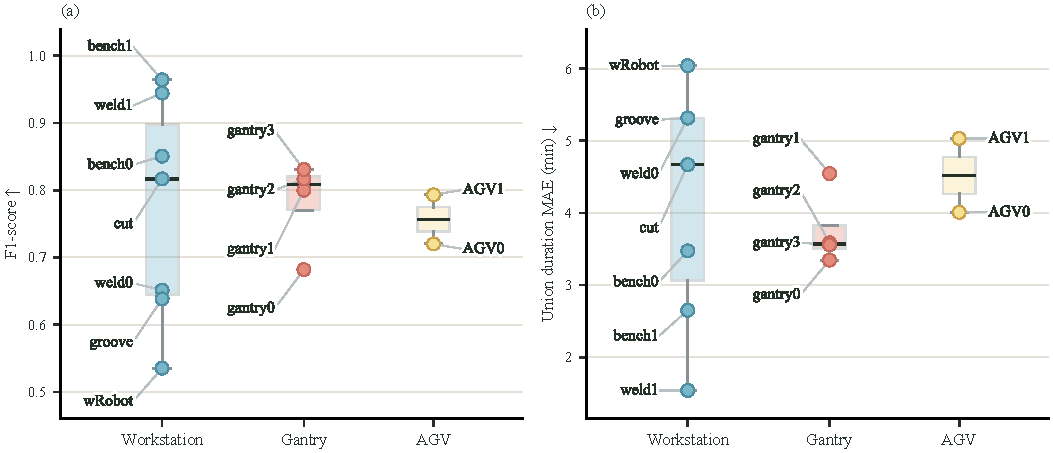
\includegraphics[width=0.95\linewidth,height=0.66\textheight,keepaspectratio]{figures/fig_per_device_box.pdf}
\captionsetup{hypcap=false}
\captionof{figure}{Per-device F1-score and union duration MAE for PHGST-DM at Onset limit~$\leq5$, grouped by resource type: workstation, gantry, and AGV.}
\label{fig:per-device}
\end{center}




% The chapter records implementation challenges and the design responses used in this project.
\chapter{Challenges}
\label{ch:challenges}

Despite the progress, we encountered several challenges during the development and evaluation of the forecasting system. They involved production-system representation, supervision and evaluation, temporal dependencies, and multi-task optimization.

\begin{itemize}[leftmargin=1.7em,itemsep=0.55\baselineskip,topsep=0.35\baselineskip]
\item \textbf{Representing heterogeneous factory resources.} Workstations, workers, buffers, AGVs, gantries, and material-supply observations do not share the same semantics or operational role. Treating them as interchangeable features made it difficult to distinguish a processing constraint from a transport or supply constraint. We addressed this by building a 38-node heterogeneous process--logistics graph, using resource-type projections and semantic feature groups, and keeping geographic and semantic relations separate. The NoGraph, NoGroup, NoCross, and NoInfo ablations helped check whether the representation preserved useful cross-resource information.

\item \textbf{Constructing process-informed bottleneck labels.} The main difficulty was converting noisy process signals into labels that reflect a sustained bottleneck. Queueing, blockage, starvation, worker availability, material shortage, and transport delay can overlap, and a rule that works for a workstation may be inappropriate for a gantry or transport robot. We therefore used resource-specific rules, required at least eight minutes of persistence, filled internal gaps of at most one window, and separated Upcoming from Ongoing events. These choices made the labels more consistent with sustained constraints while keeping them computable from history only.

\item \textbf{Learning from rare events under severe class imbalance.} Roughly 98\% of the test pairs are No-event, so a model can appear accurate by favouring the majority class. At the same time, aggressively recovering the few positive windows can produce unstable false alarms. We mitigated this tension with positive-window oversampling, weighted objectives, far-onset weighting, and a hard-false-positive penalty. Event F1, Upcoming/Ongoing recall, and strict onset matching complemented accuracy.

\item \textbf{Capturing delayed cross-resource effects.} Bottleneck evidence does not always appear first at the resource that will later be affected; changes in an upstream station, transport route, or buffer may become visible elsewhere only after several minutes. This made it difficult to distinguish a meaningful delayed dependency from a short-lived local fluctuation. We addressed the problem with temporal-pattern prototypes and delay-aware cross-resource attention, allowing earlier resource trajectories to condition later predictions. Corresponding ablation experiments were used to assess the effectiveness of these design choices.

\item \textbf{Balancing prediction targets with different scales.} The system had to predict station, onset, duration, cause, and remaining order time at the same time, although these targets have different types, scales, and error costs. A single training schedule could allow one objective to dominate the others or could disturb already useful event outputs when the remaining-time objective was refined. We used two-stage training: Stage~1 jointly learns the shared representation and event-related outputs, while Stage~2 freezes the encoder, event heads, and cause head and fine-tunes only the remaining-time head. This separated the optimization pressures while preserving the event and cause predictions.
\end{itemize}

% Adapted from the manuscript's Discussion and Conclusion; no new empirical claims.
\chapter{Conclusion}
\label{ch:conclusion}

This project presents PHGST-DM for joint bottleneck forecasting in multi-entity production systems. It combines a heterogeneous process--logistics graph, process-informed supervision, and recurrent-pattern-guided delay-aware modelling. The predictor reports the bottleneck station, onset, duration, observable process cause, and remaining order time, connecting resource-level constraints with order-level production progress.

In the evaluated simulation, the model achieves event F1-scores of 80.4\%, 77.8\%, and 76.8\% at onset limits of 5, 10, and 15~min, respectively. These scores exceed the strongest baseline at each limit by 8.2--22.1 percentage points. Detected-event duration MAE is lower by 0.86--1.03~min, equivalent to a 31.6\%--37.5\% reduction. Process-cause accuracy and macro recall also exceed those of the compared baselines. Fine-tuning only the remaining-time head reduces its MAE to 9.60, 9.27, and 8.91~min while retaining the event and cause outputs.

The component studies support complementary roles for the proposed designs. Broader resource observations improve advance-warning coverage; process-cause supervision improves cause identification with little change in logged station F1; and temporal-pattern clustering and prototype matching strengthen the prediction of more distant events. The sensitivity pilot provides preliminary support for label relevance. These findings remain specific to the evaluated simulation; real-factory transfer and the production benefits of forecast-guided interventions require further validation.

Future work will focus on two connected directions. The first is transfer and validation beyond the simulator. Real-factory observations or synchronized digital-twin streams should be combined with the current Isaac Sim data to test sensor noise, incomplete event logs, maintenance periods, operating-speed changes, and production-policy changes. Independently reviewed labels, sensitivity analysis for persistence and threshold choices, rare-event probability calibration, and uncertainty estimates will be needed to determine whether the resource relations and process-informed bottleneck definitions remain reliable. These comparisons can also prioritize the most informative resource signals.

The second direction is forecast-guided operational support. The current predictor reports bottleneck location, onset, duration, cause, and remaining order time, but its outputs are not yet used to change production schedules, reallocate workers or AGVs, or adjust material-transfer orders. Future evaluation should select feasible interventions under resource-capacity, execution-delay, and safety constraints, then measure their effects on bottleneck duration, order completion, and throughput. This will establish a closed loop from prediction to decision, execution, and production response.


% ==================== 参考文献及附录 ====================
% Retain the final manuscript's complete 38-reference set during collaboration.
% After Chapters 1--3 are merged, remove \nocite{*} if only report-cited works are desired.
\nocite{*}
\begingroup
\setstretch{1.10}
\setlength{\bibsep}{6pt}
\bibliographystyle{plainnat}
\bibliography{references}
\endgroup

% Adapted from the manuscript appendices; detailed attention moved from experiments.
\unnumberedchapter{Appendix}
\suppressfloats[t]
\label{ch:appendix}
\setcounter{section}{0}
\renewcommand{\thesection}{\Alph{section}}
\renewcommand{\thesubsection}{\thesection.\arabic{subsection}}
\counterwithin{figure}{section}
\counterwithin{table}{section}
\counterwithin{equation}{section}
\renewcommand{\theHsection}{appendix.\Alph{section}}
\renewcommand{\theHfigure}{appendix.\thesection.\arabic{figure}}
\renewcommand{\theHtable}{appendix.\thesection.\arabic{table}}
\renewcommand{\theHequation}{appendix.\thesection.\arabic{equation}}
\FloatBarrier
\section{Implementation Details and Additional Results}\label{app:additional}

The appendices provide implementation settings, numerical rules, supplementary prediction and case results, and descriptive attention maps.

Table~\ref{tab:shared-training-protocol} summarizes the settings shared by the Full model and ablation arms; their architectural differences are listed in Table~\ref{tab:ablation-arms}.

The exploratory station/window descriptors use eight clusters ($K=8$) and neither define event labels nor contribute a cluster-prediction loss.

\begin{table}[htbp]
\centering
\caption{Shared training, model, and task settings for the Full model and ablation arms.}
\label{tab:shared-training-protocol}
\footnotesize
\setlength{\tabcolsep}{6pt}
\renewcommand{\arraystretch}{1.05}
\begin{tabularx}{\linewidth}{@{}p{0.30\linewidth}Y@{}}
\toprule
Item & Setting \\
\midrule
Initialization and seed & Identical initial parameter values across arms; seed 42 \\
Optimizer and batch size & AdamW; batch size 16; weight decay 0.05 \\
Learning rate & $5\times10^{-5}$ initially; cosine decay to $10^{-6}$ \\
Sampling and training budget & Fourfold positive-window oversampling; at most 50 epochs per onset-limit run; early-stopping patience 40 \\
Curriculum & Onset limit~$\leq5\rightarrow$Onset limit~$\leq10\rightarrow$Onset limit~$\leq15$ \\
Checkpoint criterion & Validation station-identification F1 among candidates with report precision $\geq0.80$ and recall $\geq0.70$ \\
Threshold candidates & $\{0.45,0.50,0.55,0.60,0.65,0.70,0.75,0.80,0.85,0.88,0.90,0.94\}$ \\
Held-out evaluation & Freeze the selected checkpoint and threshold before evaluating the shared test episodes \\
Windowing and targets & 60-s windows; 30 historical and 30 future windows; seven workstation, four gantry, and four transport-robot targets \\
Event and matching rules & One-window internal gap filling; Onset limit~$\leq5/10/15$; three-window onset tolerance \\
Encoder and attention & Five blocks; hidden dimension 80; temporal/geographic/semantic heads $4/2/2$ \\
Graph and positional context & Geographic hop cutoff 4; five semantic neighbours; eight-dimensional Laplacian encoding \\
Pattern bank & 16 prototypes from length-three temporal patches \\
Far-onset enhancement & Onset-loss multiplier 2; positive weights $9/10/11$ for Onset limit~$\leq5/10/15$ \\
False-alarm weighting & Ordinary false-positive weight 2.5; additional hard-false-positive multiplier 2.2 \\
\bottomrule
\end{tabularx}
\end{table}

The joint training objective uses the following weights. Event occurrence, start, duration, and prefix losses have weights $2.4$, $2.0$, $2.0$, and $2.5$, respectively. The cold-history onset term has weight $2.2$ within the event-occurrence objective; focal modulation uses exponent $1.5$, and the internal differentiable F1 term has weight $0.8$. Future occupancy uses separate binary-cross-entropy, Dice, and IoU weights of $0.7$, $0.5$, and $0.35$. The reconstruction, supervised contrastive, cause, and turning-point/momentary losses have weights $0.2$, $0.05$, $0.1$, and $0.25$. Remaining-time regression has weight $0.5$ in stage~1 and $4.0$ during head-only stage~2.

The offline event CSV can retain a one-window event through score-event merging. PHGST-DM training instead constructs targets from the operational occupancy grid.

All state rules act on the original physical feature scale before input standardization. Let $q$, $B$, $S$, $U$, $I$, $R$, and $Z$ denote queue length, blocked seconds, starved seconds, unavailable fraction, inbound-wait seconds, route-delay seconds, and shortage propagation, respectively. At the 60-s resolution, a workstation has raw hot evidence if any of the following holds: (i) $q\geq2$ and $B+S>0$; (ii) $B\geq24$ and $q\geq1$; (iii) $B+S\geq24$ together with an upstream/downstream coupling ratio of at least $0.15$, $I\geq20$, $R\geq20$, $Z\geq0.25$, or $q\geq1$; (iv) $S\geq30$ and $Z\geq0.25$; (v) $S\geq18$ and either $I\geq20$ or $R\geq20$; or (vi) $B+S\geq24$ together with worker absence or labour saturation. An active workstation operating-variation flag combined with $U\geq0.5$ also supplies hot evidence. Worker absence uses unavailable fraction $\geq0.5$; labour saturation uses an activity cutoff of $0.8$ among present workers, with a presence tolerance of $0.05$. A gantry requires $B+S\geq18$ and either $I\geq20$ or $R\geq20$, whereas a transport robot requires $B+S\geq18$ and $I\geq20$; either handling type is also hot when $U\geq0.5$. When an operating-variation flag is active, evidence is retained only if $q\geq1$, $B+S\geq24$, or $U\geq0.5$. Raw indicators are filtered to remove runs shorter than eight one-minute windows, after which internal gaps of at most one window are filled. This retrospective occupancy grid supplies supervision; inference uses only the observed prefix.

For correspondence with the code, the disabled auxiliary-loss switches retain the implementation names \texttt{score}, \texttt{will}, \texttt{mark}, \texttt{time-to-start}, \texttt{STGNPP}, and \texttt{offline cluster-head}. These names identify inactive configuration options; the active occurrence loss $\mathcal{L}_{\mathrm{will}}$ remains part of the training objective. The offline cluster-head weight is zero, so the model is not trained to classify the offline clustering assignments.

The prefix-continuation cutoff is $1.5$ windows. Occupancy-run extraction for event union uses probability cutoff $0.45$, with both ongoing and upcoming union enabled; direct occupancy-state evaluation uses cutoff $0.55$. The configured gantry and transport-robot report thresholds are $0.72$ and $0.68$, respectively, alongside the validation-selected global operating point. Threshold selection first prefers candidates satisfying the validation precision requirement and then maximizes the configured station-identification F1; if none satisfies that requirement, it retains the highest-F1 validation candidate. The checkpoint precision/recall gates are applied separately. If no gated checkpoint is obtained throughout training, the retained ungated checkpoint with the best validation selection score is used. Neither fallback uses test predictions or test labels.

Evaluation counts refer to forecast-origin--resource pairs, so a persistent event may contribute at successive origins. Overlapping windows are not treated as independent observations for significance testing.

\FloatBarrier
\section{Supplementary prediction results}\label{app:supplementary-results}

\subsection{Temporal and resource-type results}

For Onset limit~$\leq15$, strict report recall is $0.574/0.522/0.433$ for onset distances within 5, 6--10, and beyond 10~min. Across the three limit-specific tasks, exact-onset accuracy among station-matched true positives is $0.896/0.844/0.831$, and onset-bucket accuracy is $0.921/0.918/0.920$. Workstation/gantry/robot F1 is $0.805/0.811/0.771$ at Onset limit~$\leq5$ and $0.751/0.840/0.639$ at Onset limit~$\leq15$. Aggregate event and timing results are in Table~\ref{tab:comparison-main}.

\subsection{Structural and pattern-modelling comparisons}

Beyond the main structural-ablation results, NoGroup has a strict report recall of $0.192$ for onsets beyond 10~min. Across limits, resource-type hmean is $0.505$--$0.536$ for Full, $0.360$--$0.384$ for NoGraph, and $0.365$--$0.396$ for NoCross. Figure~\ref{fig:key-device-entity} illustrates the corresponding trajectories: Full identifies both intervals about 5~min before NoInfo and WorkstationOnly, whose duration estimates remain at 6--8~min during the plotted 20-min reference plateau. NoCross reaches 14~min before declining to about 8~min.

\subsection{Stage-resolved sensitivity alignment}

Table~\ref{tab:oracle-pilot-ci} supplements Figure~\ref{fig:label-oracle-pilot} with point estimates and reported 95\% confidence intervals for the Ops labelling method. The results describe the 30-episode development pilot and should be interpreted as exploratory evidence.

\begin{table}[!htbp]

\centering
\caption{Production-sensitivity alignment of the Ops labelling method used by PHGST-DM in the development pilot.}
\label{tab:oracle-pilot-ci}
\footnotesize
\setlength{\tabcolsep}{8pt}

\renewcommand{\arraystretch}{1.1}
\begin{tabular*}{\linewidth}{@{\extracolsep{\fill}}lrr@{}}
\toprule
Metric & Point estimate & 95\% confidence interval \\

\midrule
NDCG@3 & 0.531 & [0.492, 0.570] \\
Positive Recall@2 & 55.556\% & [51.141, 59.971]\% \\
Positive Recall@3 & 68.519\% & [63.270, 73.768]\% \\
Weighted Recall@3 & 71.623\% & [66.052, 77.194]\% \\
Coverage@3$_{0.9}$ & 72.222\% & [66.974, 77.470]\% \\
\bottomrule
\end{tabular*}
\par\vspace{3pt}
\begin{minipage}{\linewidth}
\footnotesize
The pilot comprises 30 disturbance-free development episodes. These exploratory intervals do not establish superiority over the comparison methods or generalization to other disturbance conditions.
\end{minipage}
\end{table}



The mean weighted coverage of positive sensitivity by the top three candidates is $71.6\%$ under the pilot protocol. Early-, middle-, and late-stage NDCG@3 values are $0.421/0.339/0.770$, with the strongest alignment near order completion. 

\FloatBarrier
\section{Case selection and additional resource-level results}\label{app:case-details}

\subsection{Case selection and detailed trace observations}

The episode used for the main case study is \texttt{n10\_human1.0\_\_episode\_03}. The cutting workstation contributes 301 event-positive window--resource pairs. Devices with at least the median event count are first retained. Among them, the device with the most events in a single episode is selected, with ties resolved by PHGST-DM one-step F1. Its episode is then chosen based on the number and length of bottleneck segments. Figure~\ref{fig:key-device-baselines} reports the selected case. PHGST-DM estimates the short-event duration as 10--11~min; during the plotted 20-min reference plateau, estimates are 13--17~min, with state errors spanning 1--2 boundary windows. Plot truncation does not alter the 30-min prediction horizon.

\paragraph*{Mixed-condition probability map.}
Figure~\ref{fig:attn-prediction} uses a supplementary mixed-condition checkpoint and episode \texttt{n10\_mix\_all1.0\_\_episode\_03}, selected automatically for high bottleneck activity. It shows relative test windows $0$--$200$ across 20 rows: 15 target resources and five worker context nodes, omitting 18 buffers. The panels compare future labels, probabilities, and absolute errors. Probabilities are not thresholded reports, and this supplementary configuration does not represent the aggregate performance of the main \texttt{dense\_i1} model.

\begin{figure}[!htbp]
\centering
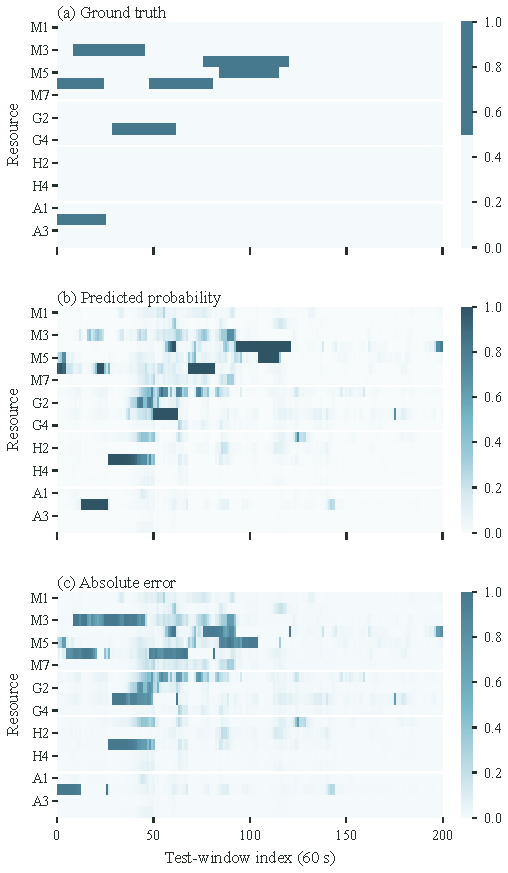
\includegraphics[width=\columnwidth,height=0.55\textheight,keepaspectratio]{figures/attention_heatmaps/fig08_prediction_heatmaps.pdf}
\caption{Future-event labels, predicted probabilities, and absolute errors for a mixed-condition episode (Onset limit~$\leq5$).}
\label{fig:attn-prediction}
\end{figure}

\paragraph*{Resource-level coverage.}

Table~\ref{tab:complete-6-1} provides per-resource counts and errors under the onset-qualified matching rule used in Table~\ref{tab:comparison-main}. Zero-support resources \texttt{robot\_2} and \texttt{robot\_3} are omitted. In this table, $n_{\mathrm{true}}$ and $n_{\mathrm{pred}}$ count reference and predicted event-positive forecast-origin--resource pairs, $P$ and $R$ denote precision and recall, and Dur MAE and Dur RMSE denote union duration errors in minutes. Device identifiers retain the simulator names so individual resources can be traced across data exports.

% Author confirms overall F1 = 80.4 percent and the same matching criterion as the main table.
% Per-device server exports are pending synchronization; do not infer replacement device counts from the aggregate score.
\begin{table}[!tbp]
\centering
\footnotesize
\setlength{\tabcolsep}{3pt}
\renewcommand{\arraystretch}{1.12}
\caption{Per-device event and duration performance at Onset limit~$\leq5$. Durations are in minutes. Zero-support resources (\texttt{robot\_2}, \texttt{robot\_3}) are omitted.}
\label{tab:complete-6-1}
\begin{tabularx}{\textwidth}{@{}lXXXXXXX@{}}
\toprule
Device & $n_{\mathrm{true}}$ & $n_{\mathrm{pred}}$ & $P$ & $R$ & F1-score & Dur MAE & Dur RMSE \\
\midrule
num00\_weld\_ws0 & 115 & 100 & 70.0\% & 60.9\% & 65.1\% & 5.31 & 7.11 \\
num00\_weld\_ws1 & 17 & 19 & 89.5\% & 100.0\% & 94.4\% & 1.54 & 2.76 \\
num01\_robotweld\_ws0 & 46 & 25 & 76.0\% & 41.3\% & 53.5\% & 6.04 & 7.56 \\
num02\_CNC$^\ast$\_ws0 & 301 & 343 & 76.7\% & 87.4\% & 81.7\% & 4.67 & 6.45 \\
num04\_groove\_ws0 & 20 & 27 & 55.6\% & 75.0\% & 63.8\% & 5.32 & 6.87 \\
num08\_bench\_ws0 & 186 & 162 & 91.4\% & 79.6\% & 85.1\% & 3.47 & 5.02 \\
num08\_bench\_ws1 & 94 & 101 & 93.1\% & 100.0\% & 96.4\% & 2.65 & 3.65 \\
gantry\_0 & 18 & 26 & 57.7\% & 83.3\% & 68.2\% & 3.35 & 4.85 \\
gantry\_1 & 31 & 34 & 76.5\% & 83.9\% & 80.0\% & 4.55 & 6.45 \\
gantry\_2 & 108 & 132 & 74.2\% & 90.7\% & 81.7\% & 3.59 & 5.56 \\
gantry\_3 & 121 & 127 & 81.1\% & 85.1\% & 83.1\% & 3.56 & 5.04 \\
robot\_0 & 15 & 10 & 90.0\% & 60.0\% & 72.0\% & 4.01 & 6.14 \\
robot\_1 & 30 & 28 & 82.1\% & 76.7\% & 79.3\% & 5.03 & 6.80 \\
\bottomrule
\end{tabularx}
\end{table}


\FloatBarrier
\section{Supplementary attention analysis}\label{app:attention-analysis}

\subsection{Historical attention and onset-limit comparisons}
Figure~\ref{fig:attn-temporal} compares historical attention under normal and upcoming bottleneck conditions using the protocol in Section~\ref{sec:attention-protocol}. Both maps contain prominent bands around history steps 12--15 and 25--30, indicating that the model draws on multiple historical regions. The upcoming-minus-normal map shows localized increases and decreases around these bands. This pattern is consistent with selective use of historical operating context when forecasting an emerging bottleneck.

\begin{figure}[hbp]
\centering
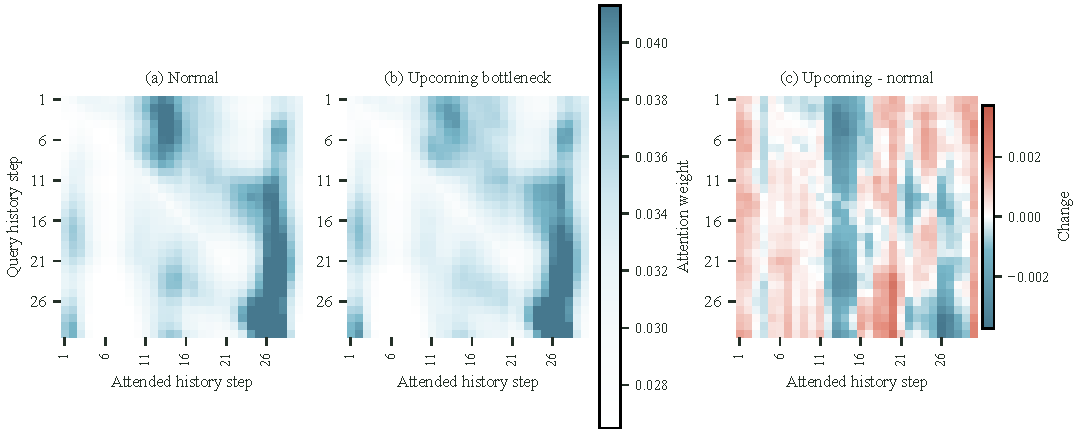
\includegraphics[width=0.98\textwidth,height=0.66\textheight,keepaspectratio]{figures/attention_heatmaps/fig04_temporal_attention_states.pdf}
\caption{Temporal attention over 30 history windows: (a)~normal; (b)~upcoming; (c)~upcoming-minus-normal.}
\label{fig:attn-temporal}
\end{figure}

\begin{figure}[!tbp]
\centering
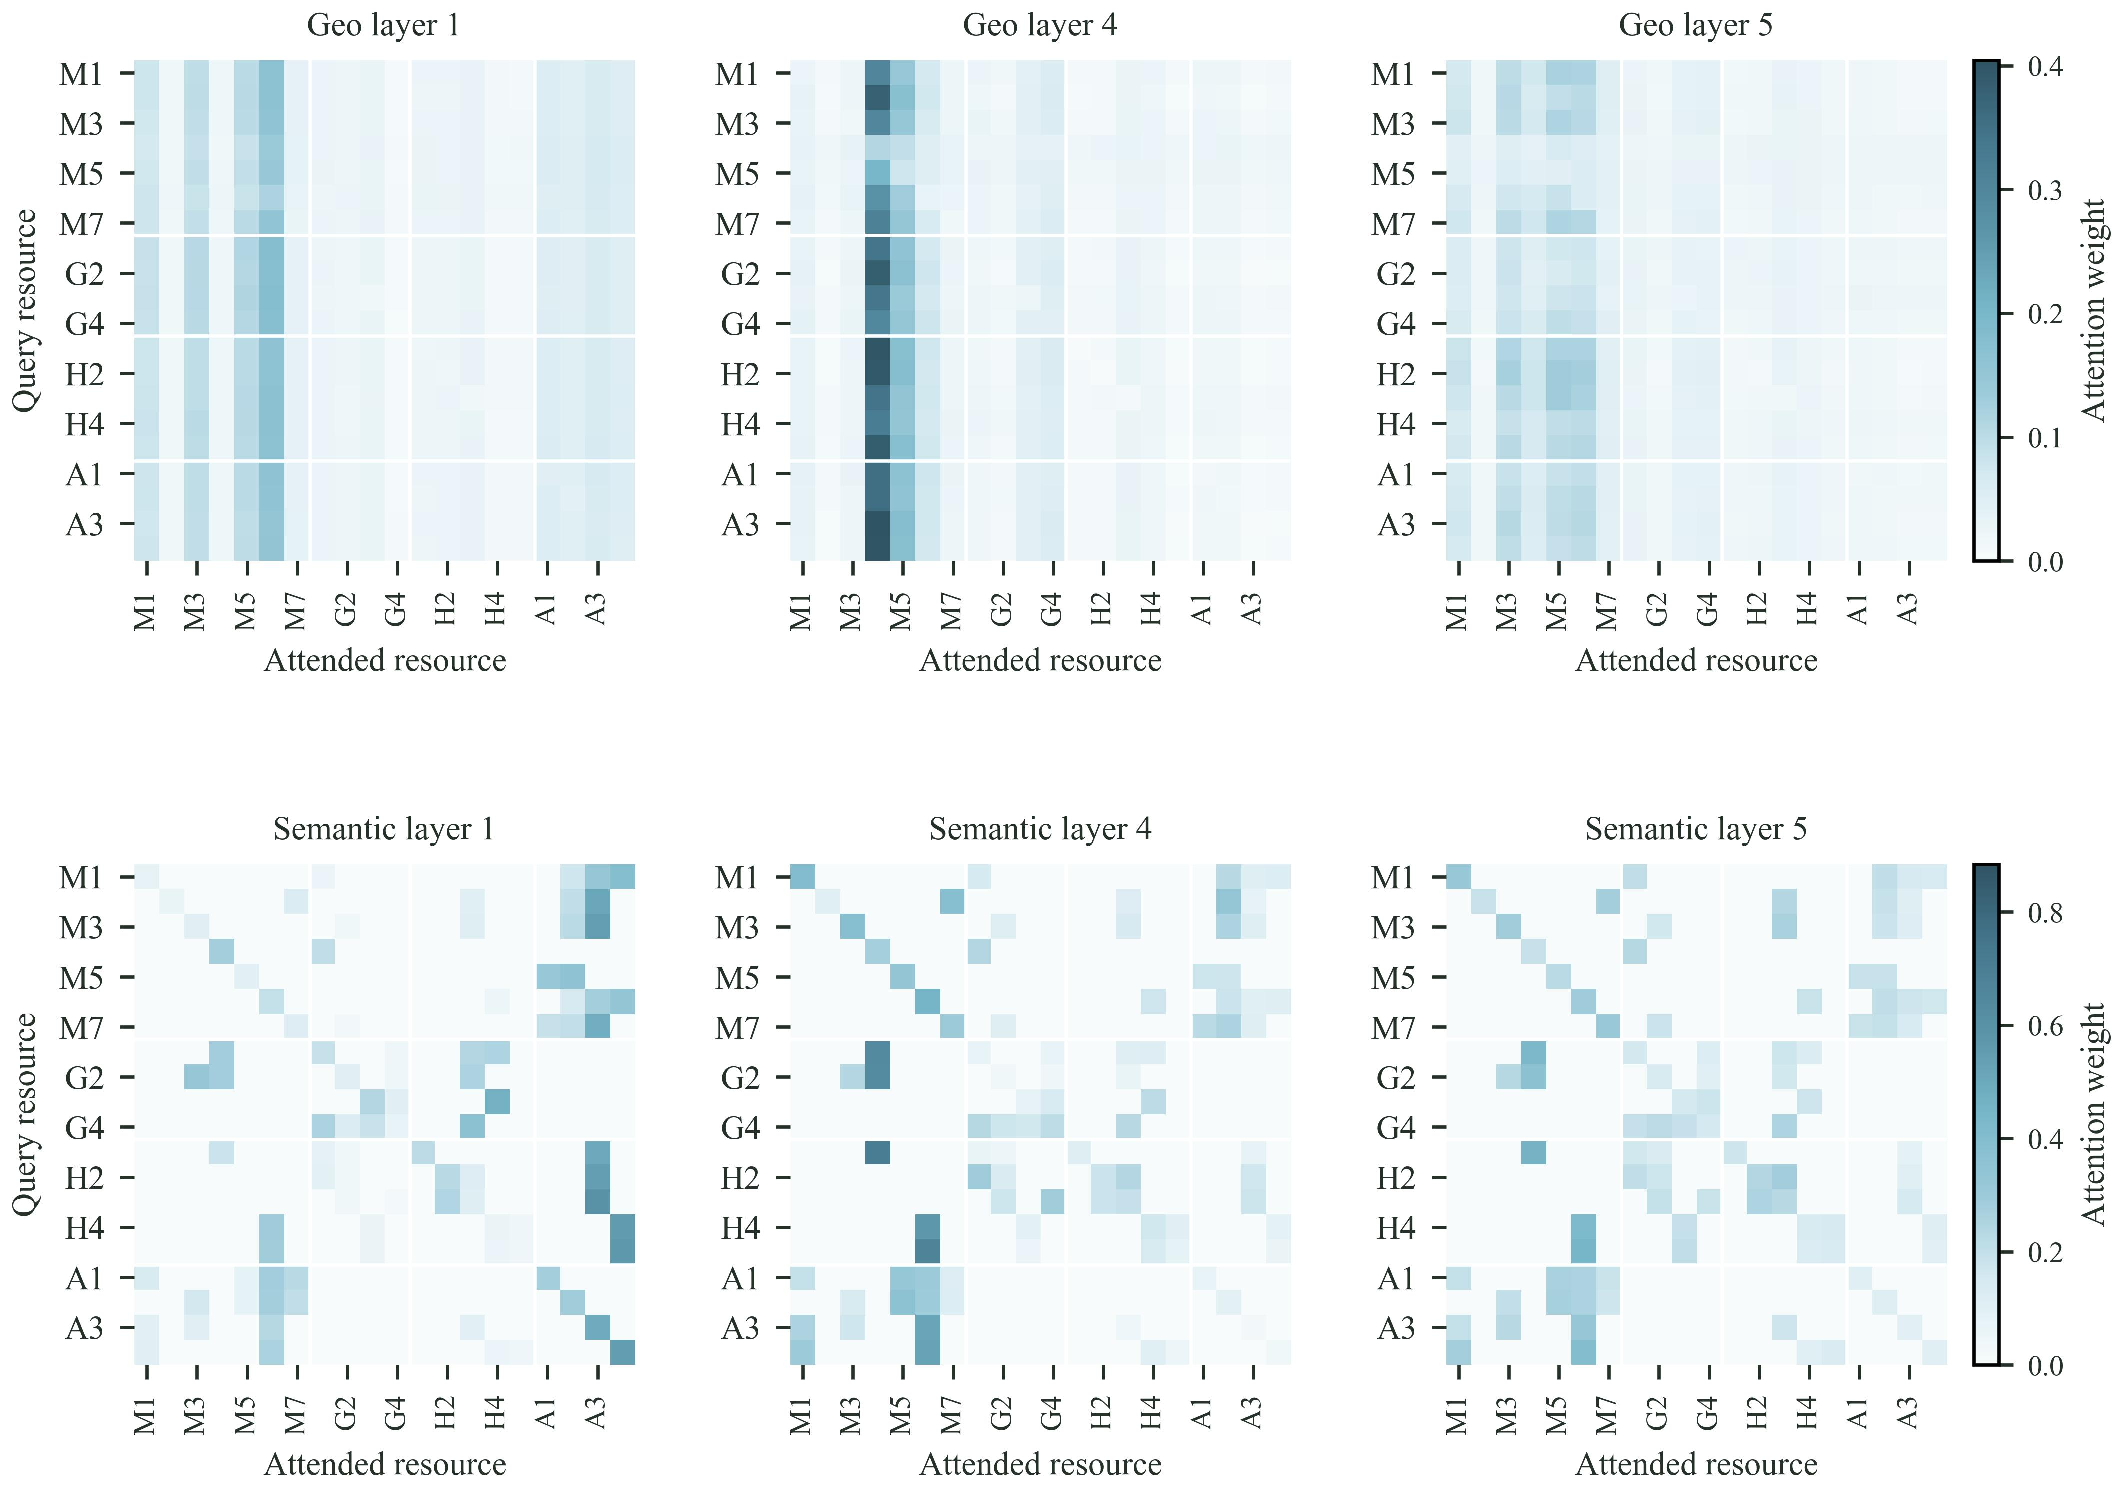
\includegraphics[width=0.92\textwidth,height=0.66\textheight,keepaspectratio]{figures/attention_heatmaps/fig05_layerwise_upcoming_attention_selected.pdf}
\caption{Geographic (upper) and semantic (lower) attention in selected encoder layers 1, 4, and 5.}
\label{fig:attn-layers}
\end{figure}

Figure~\ref{fig:attn-layers} reveals complementary changes across encoder layers. Geographic attention is distributed across several workstation columns in layer~1, becomes concentrated around M3 in layer~4, and is more distributed again in layer~5. Semantic attention remains sparse and resource-specific, with prominent links involving workstations, workers, and AGVs. Together, these views show that resource information is reweighted across layers and combined through distinct geographic and semantic patterns. Appendix~\ref{app:layerwise-attention} presents all five layers.

Figure~\ref{fig:attn-horizons} compares upcoming-minus-normal resource attention under Onset limit~$\leq5/10/15$, using 96 samples per condition. Geographic maps retain a common emphasis on the M3--M5 workstation region, while the magnitudes and extent of the changes vary across onset limits. Semantic maps show localized positive and negative changes, including recurring links to M3--M4 across resource types. Thus, the models share recurring resource associations while adjusting the allocation of attention to the admissible onset range.

\begin{figure}[!tbp]
\centering
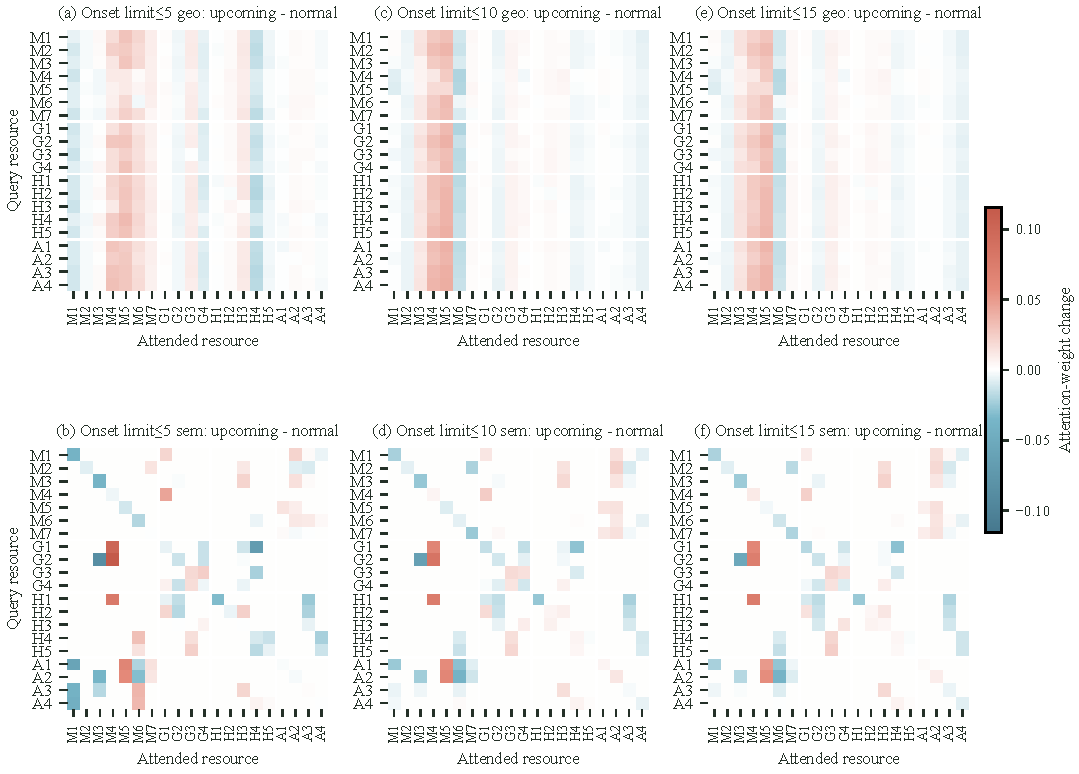
\includegraphics[width=0.98\textwidth,height=0.66\textheight,keepaspectratio]{figures/attention_heatmaps/fig07_horizon_attention_change.pdf}
\caption{Upcoming-minus-normal attention change across onset limits 5/10/15 (upper: geographic; lower: semantic).}
\label{fig:attn-horizons}
\end{figure}

\paragraph*{Learned cross-resource allocation under mixed operating conditions.}
Attention sampling and averaging follow the protocol in Section~\ref{sec:attention-protocol}. Figure~\ref{fig:attn-change} presents the resource-level change maps underlying the type-level summary in the main text.

Average attention under upcoming and ongoing conditions is compared with that under normal conditions. Colour indicates increased or decreased weight; the absolute reference matrices are retained below.

\begin{figure}[!htbp]
\centering
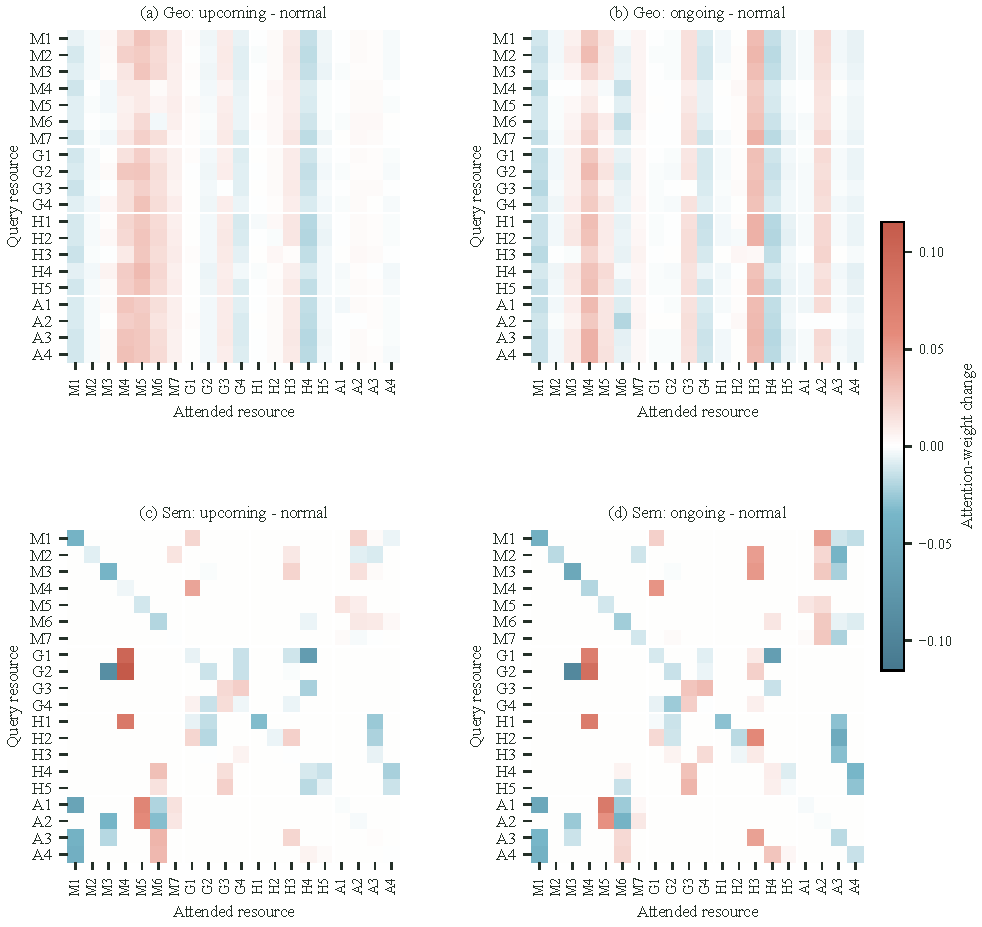
\includegraphics[width=0.92\textwidth,height=0.66\textheight,keepaspectratio]{figures/attention_heatmaps/fig03_resource_attention_change.pdf}
\caption{Redistribution of resource attention under upcoming and ongoing conditions relative to normal conditions (coral: increase; blue: decrease).}
\label{fig:attn-change}
\end{figure}



\subsection{Complete resource and layer matrices}
\label{app:absolute-attention}
\label{app:layerwise-attention}
Figures~\ref{fig:attn-states} and~\ref{fig:attn-layers-all} retain the absolute resource averages and all five layers corresponding to the selected views in this appendix. Layer-wise matrices share the same scale within each branch. Attention weights describe learned associations, not causal effects or layer-wise accuracy contributions.

\begin{figure}[!tbp]
\centering
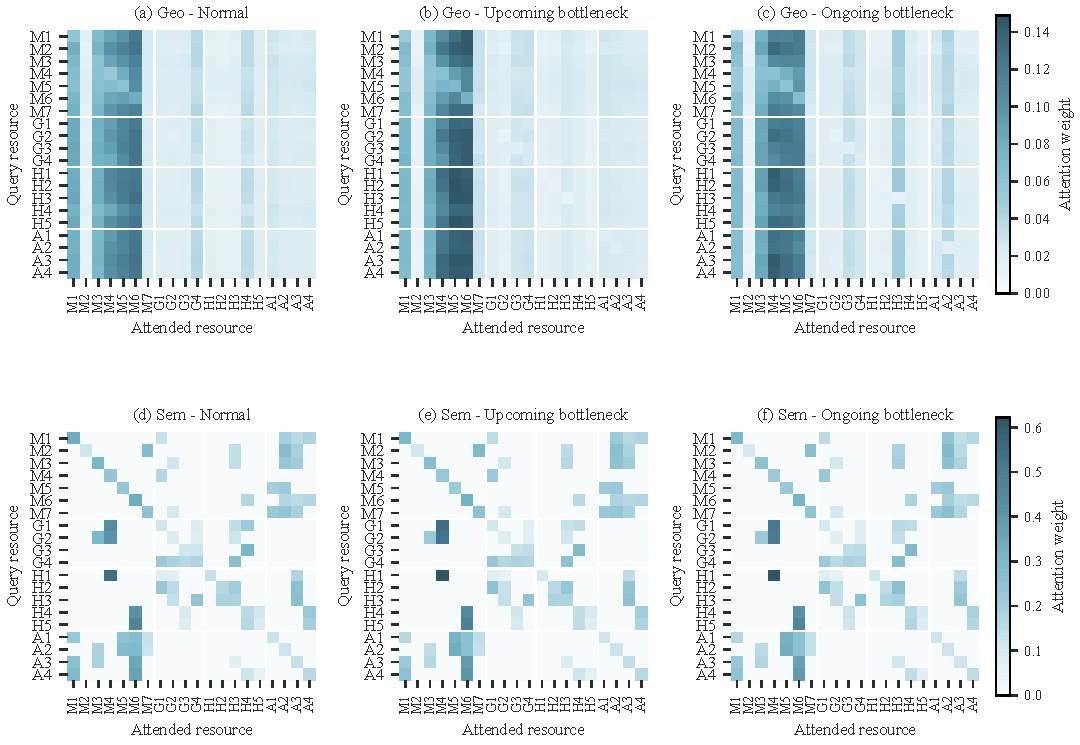
\includegraphics[width=0.92\textwidth,height=0.66\textheight,keepaspectratio]{figures/attention_heatmaps/fig02_resource_attention_states.pdf}
\caption{Absolute geographic (upper) and semantic (lower) resource attention under normal, upcoming, and ongoing conditions.}
\label{fig:attn-states}
\end{figure}

\begin{figure}[!tbp]
\centering
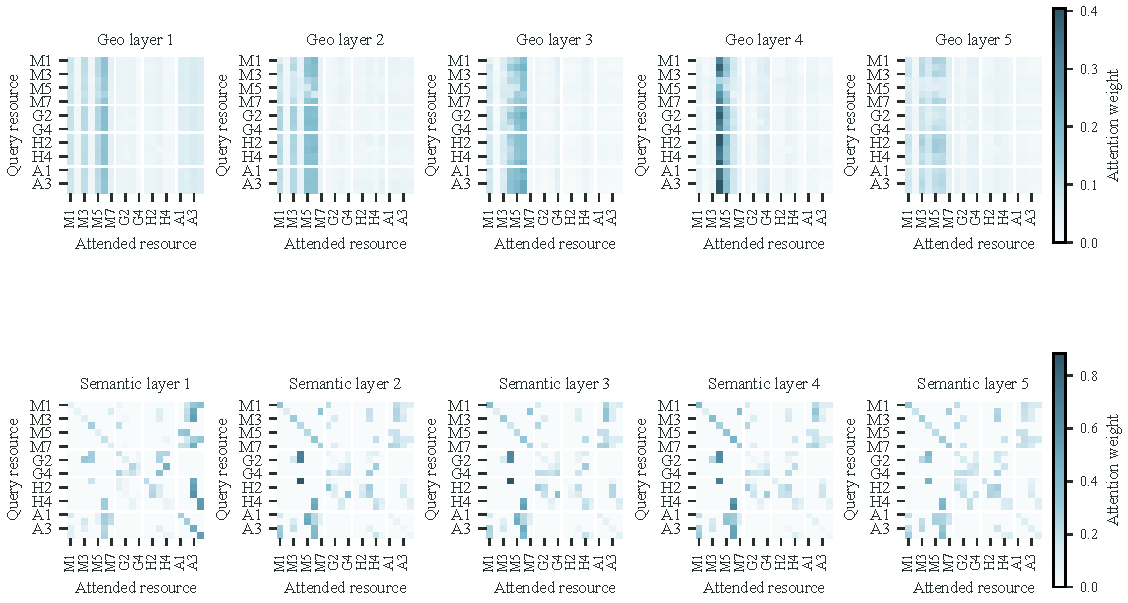
\includegraphics[width=0.94\textwidth,height=0.66\textheight,keepaspectratio]{figures/attention_heatmaps/fig05_layerwise_upcoming_attention.pdf}
\caption{Geographic (upper) and semantic (lower) attention across encoder layers 1--5 for upcoming samples.}
\label{fig:attn-layers-all}
\end{figure}



% ==================== 可选：工作分工表 ====================
% 按参考 PDF 的实际顺序放在最后。以下为可编辑重排版，不是官方原表。
% 参考 PDF 内表格说明提到致谢后放置；最终位置按你的课程要求调整。
% 签名与日期留空，由成员自行填写。
\ifincludeworkdistribution
\clearpage
\thispagestyle{empty}
\phantomsection
\addcontentsline{toc}{chapter}{Work Distribution Form}
\begingroup
\setstretch{1.0}
\begin{center}
  THE UNIVERSITY OF HONG KONG\\[2pt]
  DEPARTMENT OF MATHEMATICS,\\[2pt]
  DEPARTMENT OF STATISTICS AND ACTUARIAL SCIENCE \&\\[2pt]
  DEPARTMENT OF COMPUTER SCIENCE\\[14pt]
  \textbf{\CourseName}\\[4pt]
  \textbf{Work Distribution Form}
\end{center}
\vspace{12pt}
\noindent\textbf{I. WORK DISTRIBUTION}\par
\vspace{8pt}
\noindent Record each member's responsible chapters or project components.
For shared work, specify each member's contribution percentage.\par
\vspace{12pt}
\renewcommand{\arraystretch}{1.2}
\noindent\begin{tabularx}{\linewidth}{|p{0.25\linewidth}|Y|}
  \hline
  \textbf{Name} & \textbf{Responsible Chapters / Parts (\%)} \\
  \hline
  1.\rule{0pt}{25mm} & \\
  \hline
  2.\rule{0pt}{25mm} & \\
  \hline
  3.\rule{0pt}{25mm} & \\
  \hline
  4.\rule{0pt}{25mm} & \\
  \hline
\end{tabularx}
\vspace{22pt}

\noindent\textbf{II. STUDENTS' SIGNATURE}\par
\vspace{18pt}
\noindent\begin{tabularx}{\linewidth}{@{}XX@{}}
  1. \hrulefill & 2. \hrulefill \\[20pt]
  3. \hrulefill & 4. \hrulefill
\end{tabularx}
\vspace{18pt}

\noindent Date: \rule{0.42\linewidth}{0.4pt}
\endgroup
\fi

\end{document}
